% ******************************* PhD Thesis Template **************************
% Please have a look at the README.md file for info on how to use the template

\documentclass[a4paper,11pt,custombib]{PhDThesisPSnPDF}

% ******************************************************************************
% ******************************* Class Options ********************************
% *********************** See README for more details **************************
% ******************************************************************************

% `a4paper'(The University of Cambridge PhD thesis guidelines recommends a page
% size a4 - default option) or `a5paper': A5 Paper size is also allowed as per
% the Cambridge University Engineering Deparment guidelines for PhD thesis
%
% `11pt' or `12pt'(default): Font Size 10pt is NOT recommended by the University
% guidelines
%
% `oneside' or `twoside'(default): Printing double side (twoside) or single
% side.
%
% `print': Use `print' for print version with appropriate margins and page
% layout. Leaving the options field blank will activate Online version.
%
% `index': For index at the end of the thesis
%
% `draftclassic': For draft mode without loading any images (same as draft in book)
%
% `draft': Special draft mode with line numbers, images, and water mark with
% timestamp and custom text. Position of the text can also be modified.
%
% `abstract': To generate only the title page and abstract page with
% dissertation title and name, to submit to the Student Registry
%
% `chapter`: This option enables only the specified chapter and it's references
%  Useful for review and corrections.
%
% ************************* Custom Page Margins ********************************
%
% `custommargin`: Use `custommargin' in options to activate custom page margins,
% which can be defined in the preamble.tex. Custom margin will override
% print/online margin setup.
%
% *********************** Choosing the Fonts in Class Options ******************
%
% `times' : Times font with math support. (The Cambridge University guidelines
% recommend using times)
%
% `fourier': Utopia Font with Fourier Math font (Font has to be installed)
%            It's a free font.
%
% `customfont': Use `customfont' option in the document class and load the
% package in the preamble.tex
%
% default or leave empty: `Latin Modern' font will be loaded.
%
% ********************** Choosing the Bibliography style ***********************
%
% `authoryear': For author-year citation eg., Krishna (2013)
%
% `numbered': (Default Option) For numbered and sorted citation e.g., [1,5,2]
%
% `custombib': Define your own bibliography style in the `preamble.tex' file.
%              `\RequirePackage[square, sort, numbers, authoryear]{natbib}'.
%              This can be also used to load biblatex instead of natbib
%              (See Preamble)
%
% **************************** Choosing the Page Style *************************
%
% `default (leave empty)': For Page Numbers in Header (Left Even, Right Odd) and
% Chapter Name in Header (Right Even) and Section Name (Left Odd). Blank Footer.
%
% `PageStyleI': Chapter Name next & Page Number on Even Side (Left Even).
% Section Name & Page Number in Header on Odd Side (Right Odd). Footer is empty.
%
% `PageStyleII': Chapter Name on Even Side (Left Even) in Header. Section Number
% and Section Name in Header on Odd Side (Right Odd). Page numbering in footer

% Uncomment to change page style
%\pagestyle{PageStyleII}

% ********************************** Preamble **********************************
% Preamble: Contains packages and user-defined commands and settings
% ******************************************************************************
% ****************************** Custom Margin *********************************

% Add `custommargin' in the document class options to use this section
% Set {innerside margin / outerside margin / topmargin / bottom margin}  and
% other page dimensions
\ifsetCustomMargin
  \RequirePackage[left=37mm,right=30mm,top=35mm,bottom=30mm]{geometry}
  \setFancyHdr % To apply fancy header after geometry package is loaded
\fi

% Add spaces between paragraphs
%\setlength{\parskip}{0.5em}
% Ragged bottom avoids extra whitespaces between paragraphs
\raggedbottom
% To remove the excess top spacing for enumeration, list and description
%\usepackage{enumitem}
%\setlist[enumerate,itemize,description]{topsep=0em}

% *****************************************************************************
% ******************* Fonts (like different typewriter fonts etc.)*************

% Add `customfont' in the document class option to use this section

\ifsetCustomFont
  % Set your custom font here and use `customfont' in options. Leave empty to
  % load computer modern font (default LaTeX font).
  %\RequirePackage{helvet}

  % For use with XeLaTeX
  %  \setmainfont[
  %    Path              = ./libertine/opentype/,
  %    Extension         = .otf,
  %    UprightFont = LinLibertine_R,
  %    BoldFont = LinLibertine_RZ, % Linux Libertine O Regular Semibold
  %    ItalicFont = LinLibertine_RI,
  %    BoldItalicFont = LinLibertine_RZI, % Linux Libertine O Regular Semibold Italic
  %  ]
  %  {libertine}
  %  % load font from system font
  %  \newfontfamily\libertinesystemfont{Linux Libertine O}
\fi

% *****************************************************************************
% **************************** Custom Packages ********************************

% ************************* Algorithms and Pseudocode **************************

%\usepackage{algpseudocode}


% ********************Captions and Hyperreferencing / URL **********************

% Captions: This makes captions of figures use a boldfaced small font.
%\RequirePackage[small,bf]{caption}

\RequirePackage[labelsep=space,tableposition=top]{caption}
\renewcommand{\figurename}{Fig.} %to support older versions of captions.sty

\usepackage[ruled,vlined]{algorithm2e}
%%% Coloring the comment as blue
\newcommand\mycommfont[1]{\footnotesize\ttfamily\textcolor{blue}{#1}}
\SetCommentSty{mycommfont}

\SetKwInput{KwInput}{Input}                % Set the Input
\SetKwInput{KwOutput}{Output}              % set the Output

% *************************** Graphics and figures *****************************
\usepackage{graphicx}

%\usepackage{rotating}
%\usepackage{wrapfig}

% Uncomment the following two lines to force Latex to place the figure.
% Use [H] when including graphics. Note 'H' instead of 'h'
%\usepackage{float}
%\restylefloat{figure}

% Subcaption package is also available in the sty folder you can use that by
% uncommenting the following line
% This is for people stuck with older versions of texlive
%\usepackage{sty/caption/subcaption}
\usepackage{subcaption}

% ********************************** Tables ************************************
\usepackage{booktabs} % For professional looking tables
\usepackage{multirow}

%\usepackage{multicol}
%\usepackage{longtable}
%\usepackage{tabularx}


% *********************************** SI Units *********************************
\usepackage{siunitx} % use this package module for SI units


% ******************************* Line Spacing *********************************

% Choose linespacing as appropriate. Default is one-half line spacing as per the
% University guidelines

% \doublespacing
% \onehalfspacing
% \singlespacing


% ************************ Formatting / Footnote *******************************

% Don't break enumeration (etc.) across pages in an ugly manner (default 10000)
%\clubpenalty=500
%\widowpenalty=500

%\usepackage[perpage]{footmisc} %Range of footnote options


% *****************************************************************************
% *************************** Bibliography  and References ********************

\usepackage{cleveref} %Referencing without need to explicitly state fig /table

% Add `custombib' in the document class option to use this section
\ifuseCustomBib
  %  \RequirePackage[square, sort, numbers, authoryear]{natbib} % CustomBib


% If you would like to use biblatex for your reference management, as opposed to the default `natbibpackage` pass the option `custombib` in the document class. Comment out the previous line to make sure you don't load the natbib package. Uncomment the following lines and specify the location of references.bib file

%\RequirePackage[backend=biber, style=numeric-comp, citestyle=numeric, sorting=nty, natbib=true]{biblatex}
\RequirePackage{sty/MyBiblatexStyle}
% \RequirePackage[hyperref,style=authoryear-comp,natbib=true,maxbibnames=10,maxcitenames=2,useeditor=false,url=false,useprefix,giveninits=false,uniquelist=false,sortcites=false,dashed=false]{biblatex}
\addbibresource{References/references.bib} %Location of references.bib only for biblatex, Do not omit the .bib extension from the filename.

\fi

% changes the default name `Bibliography` -> `References'
% \renewcommand{\bibname}{References} For biblatex we update title in thesis.tex

\usepackage{MyMathCmds}
\usepackage{amsthm}
\newtheorem{definition}{Definition}
\newtheorem{theorem}{Theorem}
\newtheorem{corollary}{Corollary}[theorem]
\newtheorem{lemma}[theorem]{Lemma}


% ******************************************************************************
% ************************* User Defined Commands ******************************
% ******************************************************************************

% *********** To change the name of Table of Contents / LOF and LOT ************

%\renewcommand{\contentsname}{My Table of Contents}
%\renewcommand{\listfigurename}{My List of Figures}
%\renewcommand{\listtablename}{My List of Tables}


% ********************** TOC depth and numbering depth *************************

\setcounter{secnumdepth}{2}
\setcounter{tocdepth}{2}


% ******************************* Nomenclature *********************************

% To change the name of the Nomenclature section, uncomment the following line

%\renewcommand{\nomname}{Symbols}


% ********************************* Appendix ***********************************

% The default value of both \appendixtocname and \appendixpagename is `Appendices'. These names can all be changed via:

%\renewcommand{\appendixtocname}{List of appendices}
%\renewcommand{\appendixname}{Appndx}

% *********************** Configure Draft Mode **********************************

% Uncomment to disable figures in `draft'
%\setkeys{Gin}{draft=true}  % set draft to false to enable figures in `draft'

% These options are active only during the draft mode
% Default text is "Draft"
%\SetDraftText{DRAFT}

% Default Watermark location is top. Location (top/bottom)
%\SetDraftWMPosition{bottom}

% Draft Version - default is v1.0
%\SetDraftVersion{v1.1}

% Draft Text grayscale value (should be between 0-black and 1-white)
% Default value is 0.75
%\SetDraftGrayScale{0.8}


% ******************************** Todo Notes **********************************
%% Uncomment the following lines to have todonotes.

\ifsetDraft
	\usepackage[colorinlistoftodos]{todonotes}
	\newcommand{\mynote}[1]{\todo[author=kks32,size=\small,inline,color=green!40]{#1}}
\else
	\newcommand{\mynote}[1]{}
	\newcommand{\listoftodos}{}
\fi

% Example todo: \mynote{Hey! I have a note}

% ******************************** Highlighting Changes **********************************
%% Uncomment the following lines to be able to highlight text/modifications.
\ifsetDraft
 \usepackage{color, soul}
 \newcommand{\hlc}[2][yellow]{{\sethlcolor{#1} \hl{#2}}}
 \newcommand{\hlfix}[2]{\texthl{#1}\todo{#2}}
\else
 \newcommand{\hlc}[2]{}
 \newcommand{\hlfix}[2]{}
\fi


% Example highlight 1: \hlc{Text to be highlighted}
% Example highlight 2: \hlc[green]{Text to be highlighted in green colour}
% Example highlight 3: \hlfix{Original Text}{Fixed Text}

% *****************************************************************************
% ******************* Better enumeration my MB*************
\usepackage{enumitem}


\makeatletter
\DeclareCiteCommand{\fullcite}
  {\defcounter{maxnames}{\blx@maxbibnames}%
    \usebibmacro{prenote}}
  {\usedriver
     {\DeclareNameAlias{sortname}{default}}
     {\thefield{entrytype}}}
  {\multicitedelim}
  {\usebibmacro{postnote}}


  \setlength\parindent{0pt}
  \setlength{\parskip}{1em}


% ************************ Thesis Information & Meta-data **********************
% Thesis title and author information, refernce file for biblatex
% ************************ Thesis Information & Meta-data **********************
%% The title of the thesis
\title{Non-Parametric Decision-Making in Non-Euclidean Spaces}
%\texorpdfstring is used for PDF metadata. Usage:
%\texorpdfstring{LaTeX_Version}{PDF Version (non-latex)} eg.,
%\texorpdfstring{$sigma$}{sigma}

%% Subtitle (Optional)
\subtitle{}

%% The full name of the author
\author{Vincent Dutordoir}

%% Department (eg. Department of Engineering, Maths, Physics)
\dept{Department of Engineering}

%% University and Crest
\university{University of Cambridge}
% Crest minimum should be 30mm.
\crest{
\includegraphics[width=0.2\textwidth]{University_Crest}}
%% Use this crest, if you are using the college crest
%% Crest long miminum should be 65mm
%\crest{
\includegraphics[width=0.45\textwidth]{University_Crest_Long}}

%% College shield [optional] 
% Crest minimum should be 30mm.
%\collegeshield{
\includegraphics[width=0.2\textwidth]{CollegeShields/Kings}}


%% Supervisor (optional)
%% for multiple supervisors, append each supervisor with the \newline command
%\supervisor{Prof. A.B. Supervisor\newline
%Prof. C.D. Supervisor}

%% Supervisor Role (optional) - Supervisor (default) or advisor
% \supervisorrole{\textbf{Supervisors: }}
%% if no title is desired:
% \supervisorrole{}

%% Supervisor line width: required to align supervisors
%\supervisorlinewidth{0.35\textwidth}

%% Advisor (optional)
%% for multiple advisors, append each advisor with the \newline command
%\advisor{Dr. A. Advisor\newline
%Dr. B. Advisor}
     
%% Advisor Role (optional) - Advisor (default) or leave empty
% \advisorrole{Advisors: }
%% if no title is required
% \advisorrole{}

%% Advisor line width: required to align supervisors
%\advisorlinewidth{0.25\textwidth}


%% You can redefine the submission text:
% Default as per the University guidelines:
% ``This dissertation is submitted for the degree of''
\renewcommand{\submissiontext}{Report submitted to be registered for the PhD Degree}

%% Full title of the Degree
\degreetitle{First-Year-Report}

%% College affiliation (optional)
\college{Jesus College}

%% Submission date
% Default is set as {\monthname[\the\month]\space\the\year}
\degreedate{August 2021} 

%% Meta information
\subject{First Year Report} \keywords{{Gaussian Processes} {Decision-Making} {Engineering} {University of
Cambridge}}


% ***************************** Abstract Separate ******************************
% To printout only the titlepage and the abstract with the PhD title and the
% author name for submission to the Student Registry, use the `abstract' option in
% the document class.

\ifdefineAbstract
 \pagestyle{empty}
 \includeonly{Declaration/declaration, Abstract/abstract}
\fi

% ***************************** Chapter Mode ***********************************
% The chapter mode allows user to only print particular chapters with references
% Title, Contents, Frontmatter are disabled by default
% Useful option to review a particular chapter or to send it to supervisior.
% To use choose `chapter' option in the document class

\ifdefineChapter
 \includeonly{Chapter5/chapter5}
\fi

% ******************************** Front Matter ********************************
\begin{document}

\frontmatter

\maketitle

% % ******************************* Thesis Dedidcation ********************************

\begin{dedication} 

I would like to dedicate this thesis to my loving parents \dots

\end{dedication}


% % ******************************* Thesis Declaration ***************************

\begin{declaration}

I hereby declare that except where specific reference is made to the work of 
others, the contents of this dissertation are original and have not been 
submitted in whole or in part for consideration for any other degree or 
qualification in this, or any other university. This dissertation is my own 
work and contains nothing which is the outcome of work done in collaboration 
with others, except as specified in the text and Acknowledgements. This 
dissertation contains fewer than 65,000 words including appendices, 
bibliography, footnotes, tables and equations and has fewer than 150 figures.

% Author and date will be inserted automatically from thesis.tex \author \degreedate

\end{declaration}


% % ************************** Thesis Acknowledgements **************************

\begin{acknowledgements}      


I would like to thank my advisor Dr.~Carl Henrik Ek, and my supervisor Professor Zoubin Ghahramani for their guidance and support during the first year of my PhD degree. Their advice has greatly shaped the form of this thesis, and at the same time it has also been a pleasure to work with them.


% Mark van der Wilk
% Nicolas Durrande
% James Hensman


\end{acknowledgements}

% ************************** Thesis Abstract *****************************
% Use `abstract' as an option in the document class to print only the titlepage and the abstract.
\begin{abstract}
This is where you write your abstract ...
\end{abstract}


% *********************** Adding TOC and List of Figures ***********************

\tableofcontents

% \listoffigures
% \listoftables

% \printnomenclature[space] space can be set as 2em between symbol and description
%\printnomenclature[3em]

% \printnomenclature

% ******************************** Main Matter *********************************
\mainmatter

\chapter{Introduction}  %Title of the First Chapter


$x \in \mathcal{X}$

hello worlds \citep{neal1992bayesian}

$\GP$

$\Reals$

$\vmu$

\begin{equation}
k(x, x') = \sum_i \lambda_i \phi_i(x) \phi_i(x')
\end{equation}
%!TEX root = ../thesis.tex

\chapter{Theoretical Framework}
\label{chapter:theoretical-framework}

This chapter discusses Gaussian processes (GP) and deep Gaussian processes (DGPs), the composite model obtained by stacking multiple GP models on top of each other. We also review how to perform approximate Bayesian inference in these models, with a particular attention to Variational Inference. We also cover the theory of postive definite kernels and the Reproducing Kernel Hilbert Spaces (RKHS) they characterise.

\section{Gaussian Processes}
\label{sec:chapter1:gp}


Gaussian processes (GPs) \citep{rasmussen2006} are non-parametric distributions over functions similar to Bayesian Neural Networks (BNNs). The core difference is that neural networks represent distributions over functions through distributions on weights, while a Gaussian process specifies a distribution on function values at a collection of input locations. This representation allows us to use an infinite number of basis functions, while still enables Bayesian inference \citep{neal1996bayesian}. 

Following from the Kolmogorov extension theorem, we can construct a real-valued stochastic process (i.e. function) on a non-empty set $\mathcal{X}$, $f: \mathcal{X} \rightarrow \Reals$, if there exists on all finite subsets $\{x_1, \ldots x_N\} \subset \mathcal{X}$, a \emph{consistent} collection of finite-dimensional marginal distributions over $f(\{x_1, \ldots, x_n\})$. For a Gaussian process, in particular, the marginal distribution over every finite-dimensional subset is given by a multivariate normal distribution. This implies that, in order to fully specify a Gaussian process, it suffice to only define the mean and covariance (kernel) function because they are the sufficient statistics for every finite-dimensional marginal distribution. We can therefore denote the GP as
\begin{equation}
  \label{eq:chapter1:def-gp}
  f \sim \GP(\mu, k),
\end{equation}
where $\mu:\mathcal{X}\rightarrow\Reals$ is the mean function, which encodes the expected value of $f$ at every $x$, $\mu(x) = \Exp{f}{f(x)}$, and $k:\mathcal{X} \times \mathcal{X} \rightarrow \Reals$ is the covariance (kernel) function that describes the covariance between function values, $k(x, x') = \Cov\left(f(x), f(x')\right)$. The covariance function has to be a symmetric, positive-definite function. The Gaussianity, and the fact that we can manipulate function values at some finite points of interest without taking the behaviour at any other points into account (the marginalisation property) make GPs particularly convenient to manipulate and use as priors over functions in Bayesian models -- as we will show next.

Throughout this report, we will consider $f$ to be the complete function, and intuitively manipulate it as an infinitely long vector. Moreover, $f(\vx) \in \Reals^N$ denotes the function evaluated at a finite set of points, whereas $f^{\setminus \vx}$ denotes another infinitely long vector similar to $f$ but excluding $f(\vx)$. From the marginalisation property it follows that integrating out over the infinitely many points that are not included in $\vx$, we obtain a valid finite-dimensional density for $f(\vx)$
\begin{equation}
p(f(\vx)) = \int p(f)\,\calcd{f^{\setminus \vx}}.
\end{equation}
In the case of GPs, this finite-dimensional marginal is given by a multivariate Gaussian distribition, fully characterised by the mean $\mu$ and the covariance function $k$
\begin{equation} 
  p(f(\vx)) = \NormDist{\vmu_{\vf}, \Kff},\quad\text{where}\quad [\vmu_\vf]_{i} = \mu(x_i)\ \text{and}\ [\Kff]_{i,j} = k(x_i, x_j).
\end{equation}
Conditioning the GP at this finite set of points leads to a conditional distribution for $f^{\setminus \vx}$, which is given by another Gaussian process
\begin{equation}
  \label{eq:chapter1:conditional}
  p(f^{\setminus \vx} \given f(\vx) = \vf) = \GP\big(\kfx^\top \Kff^{-1} (\vf - \vmu_{\vf}),\ \ k(\cdot, \cdot) -  \kfx^\top \Kff^{-1} \kfx\big),
\end{equation}
where $[\kfx]_i = k(x_i, \cdot)$. The conditional distribution over the whole function $p(f \given f(\vx) = \vf)$ has the exact same form as in \cref{eq:chapter1:conditional}. This is mathematically slightly confusing because the random variable $f(\vx)$ is included both on the left and right-hand-side of the conditioning, but the equation is technically correct \citep{matthews16}.

\subsection{The Beauty of Gaussian Process Regression: Exact Bayesian Inference}

One of the key advantages of Gaussian processes for regression is that we can perform exact Bayesian inference. % In this section we briefly discuss the general methodology of Bayesian modelling and how this is performed by GPs.
% \paragraph{Problem Defintion} 
Assume a supervised learning setting where $x \in \mathcal{X}$ (typically, $\mathcal{X} = \Reals^d$) and $y \in \Reals$, and we are given a dataset $\data = \{(x_i, y_i)\}_{i=1}^N$ of input and corresponding output pairs. For convenience, we sometimes group the inputs in $\vx = \{x_i\}_{i=1}^N$ into a single design matrix and outputs $\vy = \{y_i\}_{i=1}^N$ into a vector. We further assume that the data is generated by an unknown function $f: \mathcal{X} \rightarrow \Reals$, such that the outputs are perturbed versions of functions evaluations at the corresponding inputs: $y_i = f(x_i) + \epsilon_i$. In the case of regression we assume a Gaussian noise model $\epsilon_i \sim \NormDist{0, \sigma^2}$. We are interested in learning the function $f$ that generated the data. % We denote the evaluation of the function at all inputs as $f(\vx) \in \Reals^N$ and at a single input as $f(x_i) \in \Reals$.

% \paragraph{Bayesian Modelling}
[General introduction to Bayesian modelling]
The key idea in Bayesian modelling is to specify a prior distribution over the quantity of interest. The prior encodes what we know at that point in time about the quantity. In general term, this can be a lot or a little. We encode this information in the form of a distribution. Then, as more data becomes available, we use the rules of probability, an in particlar Bayes' rule, to update our prior beliefs and compute a posterior distribution (see \citet{mackay2003information, bisschop} for a thorough introduction).

Following the Bayesian approach, we specify a \emph{prior} over the parameters of interests, which in the case of GPs is the function itself. The prior is important because it characterises the search space over possible solutions for $f$. Through the prior, we can encode strong assumptions, such as linearity, differentiability, periodicity, etc. or any combination thereof, which makes it possible to generalise well from very limited data. Compared to (Bayesian) parametric models, it is much more convenient and intuitive to specify priors directly in \emph{function-space}, rather than on the weights of a parametric model \citep{rasmussen2006}. 

Following \cref{eq:chapter1:def-gp} the prior over function evaluations at the datapoints is defined by the covariance function $k$. As we assume a \`a-priori zero mean function $\mu$ (without loss of generality) this can be written as:
\begin{equation} 
  p(f(\vx)) = \NormDist{\vzero, \Kff},\quad\text{where}\quad [\Kff]_{i,j} = k(x_i, x_j).
  % \vmu_{\vf} \in \Reals^N\text{ and }\MK_{\vf\vf} \in \Reals^{N \times N},
\end{equation}
Given the function $f$ the likelihood factorises over datapoints and is given by a Gaussian:
\begin{equation}
  p(\vy \given f) = \prod_{i=1}^N p(y_i \given f) = \prod_{i=1}^N \NormDist{y_i \given f(x_i), \sigma^2}
\end{equation}
We can obtain the posterior over the function using Bayes' rule and the marginalisation property
\begin{align}
  p(f \given \vy) 
      &= \frac{p(f)\,p(\vy \given f)}{p(\vy)} \\
      &= p(f^{\setminus \vx} \given f(\vx)) \frac{ p(f(\vx)) \prod_{i=1}^N \NormDist{y_i \given f(x_i), \sigma^2}}{p(\vy)} \\
      &= \GP\big(\kfx^\top \Kff^{-1} \vf,\ \ k(\cdot, \cdot) -  \kfx^\top \Kff^{-1} \kfx\big), 
\end{align}
The marginal likelihood (model evidence)
\begin{equation}
  p(\vy) = \NormDist{\vy \given \vzero, \Kff + \sigma^2 \Eye}
\end{equation}

\begin{enumerate}
  \item Plot: Prior, Data, Posterior
  \item occam's razor
\end{enumerate}

\paragraph{Problems}
A common criticism for GPs is that any modification to this approach breaks the Gaussian assumption. 
\begin{enumerate}
  \item Non-Gaussian likelihoods
  \item Large datasets
  \item Transformations: log or square transform
\end{enumerate}

\paragraph{Solutions}
\begin{enumerate}
  \item Laplace
  \item Expectation Propagation
  \item Sparse Variational Inference
\end{enumerate}


\section{Approximate Inference with Sparse Gaussian Processes}

\begin{enumerate}
  \item General introduction to Variational inference \citep{blei2017variational}
variational inference (VI), where the problem of Bayesian inference is cast as an optimization problem—namely, to maximize a lower bound of the logarithm of the marginal likelihood.
  \item Sparse approximations \citep{Snelson05,quinonero2005unifying}
\end{enumerate}

\section{Interdomain Inducing Variables}

The basis functions used in the approximate posterior mean TODO ref are determined by the covariance between the inducing variables and other function evaluations $\left[c_u(\cdot)\right]_m = \Cov(f(\cdot), u_m)$. Commonly, the inducing variables are taken to be function values $u_{m} = f(w_m)$, which leads to the kernel becoming the basis function $[c_u(\cdot)]_{m} = k(\vw_m, \cdot)$. \emph{Interdomain} inducing variables \citep{lazaro2009inter} select different properties of the GP (e.g.~integral transforms $u_m = \int f(\vx) g_m(\vx)\calcd{\vx}$), which modifies this covariance (see \citep{van2020framework,Leibfried2020Tutorial} for an overview), and therefore gives control over the basis functions.
Most current interdomain methods are designed to improve computational properties \citep{hensman2017variational,burt2020variational,Dutordoir2020spherical}. Our aim is to control $c_u(\cdot)$ to be a typical NN actvation function like a ReLU or Softplus. This was also investigated by \citet{sun2021neural}, although they found less common saturating activation functions.

\subsection{Example: heavyside inducing variable}

$f \sim \GP$ defined on $\sphere^1$ (the unit circle), $f: [-\pi, \pi] \rightarrow \Reals, \theta \mapsto f(\theta)$.

kernel (Arc Cosine order 0):

\begin{equation}
  k(\theta, \theta') = \kappa(\rho) = \pi - |\theta - \theta'|
\end{equation}

\begin{equation}
  \frac{\calcd{}}{\calcd{\theta}}\Bigr|_{\theta = \theta_m} k(\theta, \theta') = 
\end{equation}

\begin{equation}
  u_m = \mathcal{L}_m(f)
\end{equation}

\begin{equation}
  \mathcal{L}_m = \frac{\calcd{}}{\calcd{\theta}}\Bigr|_{\theta = \theta_m} + \int \calcd{\theta}
\end{equation}

\begin{align}
  \Cov(u_m, f(\theta')) &= \Exp{f}{\mathcal{L}_m(f)\,f(\theta')} \\
                      &=  \mathcal{L}_m k(\theta', \cdot) \\
                      &= \frac{\calcd{}}{\calcd{\theta}}\Bigr|_{\theta = \theta_m} k(\theta', \theta) + \int_{-\pi}^\pi k(\theta', \theta) \calcd{\theta}
\end{align}



\section{Deep Gaussian Processes}

% \subsection{GPflux -- a library for deep Gaussian processes}
\fullcite{dutordoir2021gpflux}


\section{Kernels and Reproducing Kernel Hilbert Space}

Kernel have a rich history in machine learning and functional analysis. Kernels became widely noticed  by the ML community when linear SVMs [CITE] were kernelised. This means that rather than using $x\top\x'$, one uses a function $k(x, x')$, which corresonponds to an inner-product in some space $\phi(x)\top \phi(x')$. This concept is also referred to as the ``kernel trick'' in the litarture. This made SVMs a compelling model for non-linear modelling problems. Prior to the deep learning revolution that began in the late nillies, kernel SVMs sat the state of the art results in many tasks: XXX. Kernels are also used in splines, Priniciple Component Analysis (PCA), Gaussian processes and in general allow for the developement of versatile algorithms to analyse and process data. Kernels operate through pairwise comparisons on datapoints and are versitale because they do not impose strong assumptions regarding the type of data, such as vectors, graphs or strings, they operate on. In what follows, we are going to focus on the theoretical properties of Mercer kernels with the application of Gaussian processes in mind, and the infinite vector space these kernels characterise. This background material will be important for the remaining chapters of the thesis. The inspiration for this section came from course Julian Marial and review paper on XXX.

\begin{definition}
A positive definite (p.d.) kernel (or Mercer kernel [TODO]) on a set $\mathcal{X}$ is a function $k: \mathcal{X} \times \mathcal{X} \rightarrow \Reals$ that is
\begin{enumerate}
  \item symmetric $k(x, x') = k(x', x)$, and
  \item satisfies for all $x_i$, $x_j \in \mathcal{X}$ and $c \in \Reals$: $\sum_{i}\sum_j c_i c_j k(x_i, x_j)\ge 0$.
\end{enumerate}
\end{definition}
One of the simplest examples of a p.d. kernel is $k(x, x') = xx'$, where $\mathcal{X} = \Reals$. This kernel is often called the linear kernel. While being simple, as we will see through the next few theorems, the associated space of functions induced by this kernel is often too restricte
In the next theorems we will see how kernels characterise a space over functions. Some of these spaces will be very explicit. For example, we will show how the linear kernel leads to a space of functions that are also linear, i.e. of the form $x \mapsto a x + b$. Other spaces belonging to kernel will be defined in a more abstract way. 

\begin{theorem}[Aronszjan, 1950 TODO]
  \label{theorem:k-and-H}
  The kernel $k$ is a p.d. kernel on $\mathcal{X}$ i.f.f. there exists a Hilbert space $\rkhs$ and a mapping $\phi: \mathcal{X} \rightarrow \rkhs$ such that $\forall x,x' \in \mathcal{X}$:
  \begin{equation}
    k(x, x') = \langle \phi(x), \phi(x') \rangle_{\rkhs}
  \end{equation}
\end{theorem}

We want to remind the reader that a Hilbert space $\rkhs$ is a (possibly infinite) vector space with an inner product $\langle f, g \rangle_{\rkhs}$ and norm $\norm{f} = \langle f, f \rangle_{\rkhs}^{\frac{1}{2}}$, and where any Cauchy sequence in $\rkhs$ converges in $\rkhs$. A Cauchy sequence is a sequence whose elements become arbitrarly close as the sequence progresses. Intuitively, a Hilbert space can be seen as a generalisation of an Euclidian space that is infinite dimensional. In the machine learning literature, $\rkhs$ is also commonly referred to as the feature space and $\phi$ the feature map.

A Reproducing Kernel Hilbert Space (RKHS) is a special type of Hilbert space mentioned in \cref{theorem:k-and-H}. It is a space over function from $\mathcal{X}$ to $\Reals$ that are ``parameterised'' by an element in $\mathcal{X}$. In other words, a datapoint $x \in \mathcal{X}$ is mapped to a function in the RKHS: $\phi(x) \in \rkhs$. To make it more explicit we also write $\phi(x) = k_x$ to highlight that $k_x$ is another function in the space $\mathcal{X} \rightarrow \Reals$.

\begin{definition}
  Let $\mathcal{X}$ be a set and $\rkhs$ a Hilbert space with inner-product $\langle \cdot, \cdot \rangle_{\rkhs}$. The function $k: \mathcal{X} \times \mathcal{X} \rightarrow \Reals$ is called a reproducing kernel of $\rkhs$ if
  \begin{enumerate}
    \item $\rkhs$ contains all functions of the form 
    \item 
  \end{enumerate}
\end{definition}

\begin{enumerate}
  \item History: RKHS pure math and into machine learning for SVM, splines and 
  \item Positive Definite and Symmetry
  \item RKHS
  \item Bochner's theorem
  \item Mercer Decomposition
  \item Examples of RKHS
  \item RKHS through Spectral Decomposition
  \item Representer Theorem
  \item Show how sparse approximation links anchor points
\end{enumerate}

\section{Spectral Representation of Gaussian Processes}

\chapter{Spherical Harmonic Variational Gaussian Processes}
\label{chapter:vish}

\section{ArcCosine kernel and Associated Reproducing Hilber Kernel Space}
The first order Arc Cosine kernel mimics the computation of infinitely wide fully connected layers with ReLU activations. \citet{cho2009kernel} showed that for $\sigma(t) = \max(0, t)$, the covariance between function values of $f(\vx) = \sigma(\vw^\top \vx)$ for $\vw \sim \NormDist{0, d^{-1/2} \Eye_d}$ and $\vw \in \Reals^d$ is given by
\begin{equation}
\label{eq:arccosine}
    k(\vx, \vx') = \Exp{\vw}{\sigma(\vw^\top \vx)\, \sigma(\vw^\top \vx')} = \underbrace{\norm{\vx} \norm{\vx'}}_{\text{radial}}\ \underbrace{\frac{1}{\pi}\big( \sqrt{1 - t^2} + t\, (\pi - \arccos t) \big)}_{\text{angular (shape function) } s(t)},
\end{equation}
where $t = \frac{\vx^\top \vx'}{\norm{\vx}\norm{\vx'}}$. The factorisation of the kernel in a radial and angular factor leads to an RKHS consisting of functions of the form $f(\vx) = \norm{\vx}\,g(\frac{\vx}{\norm{\vx}})$, where $g(\cdot)$ is defined on the unit hypersphere $\dsphere = \{\vx \in \Reals^d: \norm{\vx}_2 = 1\}$ but fully determines the function on $\Reals^d$.

The shape function can be interpreted as a kernel itself, since it is the restriction of $k(\cdot, \cdot)$ to the unit hypersphere. Furthermore its expression only depends on the dot-product between the inputs so it is a zonal kernel (also known as a dot-product kernel \citep{bietti2020deep}). This means that the eigenfunctions of the angular part of $k(\cdot, \cdot)$ are the spherical harmonics $\sh_{n, j}$ (we index them with a level $n$ and an index within each level $j \in \{1, \dots, \dnumharmonicsforlevel\}$) \citep{wendland2005,Dutordoir2020spherical}. Their associated eigenvalues only depend on $n$:
\begin{equation}
\label{eq:compute-fourier-coefficients}
    \lambda_{n} = 
   \frac{\omega_{d}}{C_n^{(\alpha)}(1)} \int_{-1}^1 s(t)\,C_n^{(\alpha)}(t)\,(1 - t^2)^{\frac{d-3}{2}} \calcd{t},
\end{equation}
where $C_n^{(\alpha)}(\cdot)$ is the Gegenbauer polynomial\footnote{See \cref{app:sec:harmonics} for a primer on Gegenbauer polynomials and spherical harmonics.} of degree $n$, $\alpha = \frac{d-2}{2}$, $\omega_d$ is a constant that depends on the surface area of the hypersphere. Analytical expressions of $\lambda_n$ are provided in \cref{app:sec:compute-eigenvalues}.
The above implies that $k$ admits the Mercer representation:
\begin{equation}
    \label{eq:mercer}
    k(\vx, \vx') = \norm{\vx}\, \norm{\vx'} \sum_{n=0}^\infty \sum_{j=1}^{\dnumharmonicsforlevel}  \lambda_n \sh_{n, j}\left(\frac{\vx}{\norm{\vx}}\right)\, \sh_{n, j}\left(\frac{\vx'}{\norm{\vx'}}\right),
\end{equation}
and that the inner product between any two functions $g,\, h \in \rkhs$ is given by:
\begin{equation}
\label{eq:RKHSinnerproduct}
\big\langle g, h \big\rangle_{\rkhs} = 
    \sum_{n,j}
            \frac{{g}_{n, j} {h}_{n, j}}{\lambda_{n}}
\end{equation}
where $g_{n, j}$ and $h_{n, j}$ are the Fourier coefficients of $g$ and $h$, i.e. $g(\vx) = \sum_{n,j} g_{n,j} \norm{\vx} \sh_{n,j}(\vx)$.


\section{Spherical Harmonics}
\label{section:spherical-harmonics}

Spherical harmonics are a special set of functions defined on the hypersphere and play a central role in harmonic analysis and approximation theory \citep{wendland2005}. They originate from solving Laplace's equation, and form a complete set of orthogonal functions. Any sufficiently regular function defined on the sphere can be written as a sum of these spherical harmonics, similar to the Fourier series with sines and cosines. Spherical harmonics are defined in arbitrary dimensions \citep{frye2014,dai2013}, but lack explicit formulations and practical implementations in dimensions larger than three. %This is mainly due to the complexity of solving Laplace's equation in higher dimensions.

In this section, we propose a novel algorithm to construct spherical harmonics in $d$ dimensions. The algorithm is based on the existence of a fundamental system of points on the hypersphere, which we select in a greedy fashion through optimisation. This result in spherical harmonics that are a linear combination of zonal functions and form an orthnormal basis on $\dsphere$. The algorithm lends itself well for implementation in Python and TensorFlow, which we provide at: \url{https://github.com/vdutor/SphericalHarmonics}. The code is accompagnied by a series of tests that show that the properties of spherical harmonics, as detailed below, hold. Before outlining the algorithm, we briefly define and cover the important properties of spherical harmonics in $\Reals^d$. We refer the interested reader to \citet{dai2013,frye2014} for a comprehensive overview.
% exist bases of spherical harmonics consisting of entirely zonal harmonics

We adopt the usual $L_2$ inner product for functions $f: \dsphere \rightarrow \Reals$ and $g: \dsphere \rightarrow \Reals$ restricted to the sphere 
\begin{equation}
     \langle f, g\rangle_{L_{2}(\dsphere)} = \frac{1}{\darea} \int_{\dsphere} f(x)\,g(x) \, \calcd{\omega},
\end{equation}
where $\calcd{\omega(x)}$ is the surface area measure such that $\darea$ denotes the surface area of $\dsphere$ 
\begin{equation}
\label{eq:surface}
    \darea = \int_{\dsphere} \calcd{\omega(x)} = \frac{2 \pi ^ {d/2}}{\Gamma(d/2)}.
\end{equation}

Throughout this section we use the following notation and definitions. For $x = (x_1, \ldots, x_d) \in \Reals^d$ and $\alpha = (\alpha_1, \ldots, \alpha_d) \in \Naturals^d$, a monomial $x^\alpha$ is a product $x^\alpha = x_1^{\alpha_1} \ldots x_d^{\alpha_d}$, which has degree $|\alpha| = \alpha_1 + \ldots \alpha_d$. A real homogeneous polynomial $P(x)$ of degree $n$ is a linear combination of monomials of degree $n$ with real coefficients, that is $P(x) = \sum_{|\alpha| = n} c_{\alpha} x^{\alpha}$, with $c_\alpha \in \Reals$. We denote $\mathcal{P}_n^d$ as the space of real homogeneous polynomials of degree $n$, and can show that, counting the cardinality of the set $\{\alpha \in \Naturals^d: |\alpha| = n\}$, that $\dim(\mathcal{P}_n^d) = \binom{n + d -1}{n}$. A function $f:\Reals^d \rightarrow \Reals$ is said to be \emph{harmonic} if $\Delta f = 0$, where $\Delta = \partial_{x_1}^2 + \ldots + \partial_{x_d}^2$ and $\partial_{x_i}$ the partial derivate w.r.t. the $i$-th variable.

\begin{definition}
    The spherical harmonics of degree $n$ of $d$ variables, denoted by $\mathcal{H}_{n}^d$, is the linear space of harmonic and homogeneous in degree $n$ polynomials on $\dsphere$, that is 
    \begin{equation}
        \mathcal{H}_{n}^d = \{p \in \mathcal{P}_n^d: \Delta p = 0\ \text{and}\ p: \dsphere \rightarrow \Reals \}.
    \end{equation}
The dimensionality of $ \mathcal{H}_{n}^d$ is given by
\begin{equation}
\label{eq:numharmonics}
\dim(\mathcal{H}_{n}^d) = \frac{2 n + d - 2}{n} \binom{n + d - 3}{d - 1} := \dnumharmonicsforlevel.
\end{equation}
\end{definition}

The space $\mathcal{H}_{n}^d$ has an orthonormal basis consisting of $\dnumharmonicsforlevel$ functions, denoted by $\{\phi_{n,j}\}_{j=1}^{\dnumharmonicsforlevel}$. The basis satisfy the following properties
\begin{equation}
    \mathcal{H}_{n}^d  = \textrm{span}\left(\phi_{n,1}, \ldots, \phi_{n, \dnumharmonicsforlevel}\right),\quad\text{and}\quad\left\langle \phi_{n, j}, \phi_{n', j'}\right\rangle_{L_2(\dsphere)} = \delta_{n n'} \delta_{j j'}.
\end{equation}

From the completeness and orthonormality of the spherical harmonic basis $\{\phi_{n,j}\}_{n=0,j=1}^{\infty,\dnumharmonicsforlevel}$, it can be shown that they also form a basis of square-integrable functions \citep{frye2014}. This means that we can decompose a function $f: \dsphere \rightarrow \Reals$ as
\begin{equation}
    f = \sum_{n=0}^{\infty} \sum_{j=1}^{\dnumharmonicsforlevel} \widehat{f}_{n, j} \phi_{n, j},\quad\text{with}\quad\widehat{f}_{n, j} = \langle f, \phi_{n, j} \rangle_{L_2(\dsphere)},
\end{equation}
which can be seen as the spherical analogue of the Fourier decomposition of periodic functions onto a basis of sines and cosines.

Subsequently, we will coin the set $\{\phi_{n,j}\}$ as the spherical harmonics. They are indexed by $n$ and $j$, where $n=0,1,2,\ldots$ denotes the degree (or level) and $j=1,\cdots,\dnumharmonicsforlevel$ denotes the orientation of the spherical harmonic. We are interested in finding $\{\phi_{n,j}\}$ in arbitrary dimension. For $d=2$, is solving Laplace's equation ($\Delta p = 0$) directly relatively straightforward. Doing so reveals that $N^{2}_0 = 1$ with $\phi_{0, 1} = 1$ and $N^{2}_n = 2$ for all $n > 0$ with $\phi_{n, 1}(\theta) = \sqrt{2} \cos(n \theta)$ and $\phi_{n, 2}(\theta) = \sqrt{2} \sin(n \theta)$. This shows that on the unit circle $\sphere^1$, the spherical harmonics correspond to the Fourier basis. For $d=3$, we can also directly solve Laplace's diffential equation to find $\dnumharmonicsforlevel = 2n + 1$ and a closed form solution for $\{\phi_{n,j}\}$. However, for $d > 3$, explicit formulations for the spherical harmonics become very rare. To the best of our knowledge, the only explicit formulation we could find is in \citet[Theorem~5.1]{dai2013}, which consists of a product over polynomials. This makes the implementation cumbersome and numerically unstable, and only practically useful up to 10 dimensions \citep{Dutordoir2020spherical}. However, making use of the following two theorems, in \cref{sec:sec:zonal-spherical-harmonics} we can derive another formulation for the basis of spherical harmonics as a sum of polynomials, rather than a product. The connection between spherical harmonics and orthogonal polynomials becomes clear in the next theorem.
\begin{theorem}[Addition]
    \label{theorem:addition}
    Let $\{\phi_{n,j}\}_{j=1}^{\dnumharmonicsforlevel}$ be an orthonormal basis for the spherical harmonics of degree $n$ and $x,x' \in \dsphere$. Then the Gegenbauer polynomial $C_n^{(\alpha)}: [-1, 1] \rightarrow \Reals$ of degree $n$ can be written as
\begin{equation}
    \sum_{j=1}^{\dnumharmonicsforlevel} \phi_{n, j}(x) \phi _{n, j}(x') = \frac{n + \alpha}{\alpha}\,
    C_n^{(\alpha)}(x\transpose x')\quad\text{with}\quad \alpha = \frac{d-2}{2}.
\end{equation}
\end{theorem}
As a result of the relation between the Gegenbauer polynomial and the spherical harmonics, are the Gegenbauer polynomial sometimes referred to as ultraspherical polynomials. For $d=2$, Theorem~1 recovers the addition formula of the cosine function, as indeed $\cos(\theta) \cos(\theta') + \sin(\theta) \sin(\theta') = \cos(\theta - \theta')$ and $C_n^{(0)}(t) = \cos(n \arccos(t))$. The Gegenbauer polynomials with $\alpha=0$ are better known as the Chebyshev polynomials. Another connection between spherical harmonics and Gegenbauer polynomials is given by the Funk-Hecke theorem and applies to zonal functions. A zonal function on $\dsphere$ is a function that is rotationally invariant w.r.t. to a point on the sphere, $\eta \in \dsphere$. This means that the function only depends on the inner product $\eta\transpose x$, or equivalently, on the geodestic distance between $\eta$ and $x$.

\begin{theorem}[Funk-Hecke]
    % \label{appendix:theorem:funk}
    Let $f$ be an integrable function such that $\int_{-1}^1 \| f(t)\| (1 - t^2)^{(d-3)/2} \calcd{t}$ is finite and $d \ge 2$. Then for every $\phi_{n,j}$  and $\eta \in \dsphere$
    \begin{equation}
        \frac{1}{\darea} \int_{\dsphere} f(\eta\transpose x)\,\phi_{n, j}(x)\, \calcd{\omega(x)} = {\lambda}_{n}\,\phi_{n,j}(\eta),
    \end{equation}
    where ${\lambda}_{n}$ is a constant defined by
    \begin{equation}
        \lambda_{n}  = 
        % \frac{\Omega_{d-2}}{\Omega_{d-1}} 
        \frac{\omega_{d}}{C_n^{(\alpha)}(1)} \int_{-1}^1 f(t)\,C_n^{(\alpha)}(t)\,(1 - t^2)^{\frac{d-3}{2}} \calcd{t},
    \end{equation}
    with $\alpha = \frac{d-2}{2}$ and $\omega_d = \frac{\Omega_{d-2}}{\Omega_{d-1}}$.
\end{theorem}

\subsection{Zonal Spherical Harmonics}
\label{sec:zonal-spherical-harmonics}

From the Funk-Hecke and the Addition theorem, it is clear that there is a strong connection between spherical harmonics and Gegenbauer polynomials. The next theorem develops this connection further as it states that a basis for spherical harmonics can be written as zonal Gegenbauer polynomials. % , that is $\phi_{n,j}(x) = \sum_i \beta_{j,i} C_n^{(\alpha)}(\eta_i\transpose x)$. In what comes next we show how to select the weights $\beta_{j,i}$ and zonal directions $\eta_i \in \dsphere$.

\begin{theorem}
    If $\{\eta_1, \ldots, \eta_{\dnumharmonicsforlevel} \} \in \dsphere$ is a fundamental system of points on the sphere, then $\{C_n^{(\alpha)}(\eta_i \cdot)\}_{i=1}^{\dnumharmonicsforlevel}$ is a basis for $\mathcal{H}_n^d$. A collection of points $\{\eta_1, \ldots, \eta_M \} \in \dsphere$ is called a fundamental system of degree $n$ consisting of $M$ points on the sphere if
    \begin{equation}
        \label{eq:fundamental-system}
        \textrm{det}\ 
        \begin{bmatrix}
            C_n^{(\alpha)}(1) & \ldots & C_n^{(\alpha)}(\eta_1\transpose\eta_M) \\
            \vdots & & \vdots \\
            C_n^{(\alpha)}(\eta_M\transpose\eta_1) & \ldots & C_n^{(\alpha)}(1)
        \end{bmatrix} > 0.
    \end{equation}
\end{theorem}
Finding a basis for $\mathcal{H}_n^d$ is thus equivalent to finding a set of $\dnumharmonicsforlevel$ points that satisfy \cref{eq:fundamental-system}. Crucially, \citet[Lemma~3]{dai2013} show that there always exists a fundamental system of degree $n$ and $\dnumharmonicsforlevel$ points.

Following the theoreom, if we wish to construct $\{\phi_{n,j}\}_{n,j}$, an \emph{orthnormal} basis for the spherical harmonics, we firstly need a fundamental system of points. Secondly, while $\{C_n^{(\alpha)}(\eta_i \cdot)\}_{i=1}^{\dnumharmonicsforlevel}$ forms a basis for $\mathcal{H}_n^d$, the basis is not orthonormal. We will thus have to apply a Gram-Schmidt process for orthonormalising the basis. We detail both steps in the next paragraphs.

\paragraph{Construction of a fundamental system of points}
We propose to build a fundamental system of points in a greedy fashion by iteratively adding a point on the sphere that maximises the determinant as given in \cref{eq:fundamental-system}. Therefore, let $\veta = \{\eta_1, \ldots, \eta_M\}$ contain the M points that are already in the fundamental system and define the following block-matrix of size $(M+1) \times (M+1)$ as
\begin{equation}
    \renewcommand\arraystretch{1.3}
    \MM(\veta, \eta_{*}) =
    \left[
        \begin{array}{c|c}
          C_n^{\alpha}(\veta\veta\transpose) \in \Reals^{M \times M} & C_n^{(\alpha)}(\veta\eta_{*}\transpose) \in \Reals^{M \times 1} \\
          \hline
          C_n^{(\alpha)}(\veta\eta_{*}\transpose)\transpose \in \Reals^{1 \times M} & C_n^{(\alpha)}(1) \in \Reals
        \end{array}
    \right],
\end{equation}
where $C_n^{(\alpha)}(\veta\veta\transpose)$ corresponds to elementwise evaluating the Gegenbauer polynomial $C_n^{(\alpha)}: [-1, 1] \rightarrow \Reals$ for each element of $\veta \veta\transpose \in \Reals^{M \times M}$. A new point $\eta$ is added to the fundamental system if it maximises the determinant
\begin{equation}
    \eta = \argmax_{\eta_* \in \dsphere}\ \textrm{det}\left(\MM(\veta, \eta_{*})\right),
\end{equation}
in order to satisfy the condition in \cref{eq:fundamental-system}.
% \begin{equation}
%     \textrm{det}(\MC_n^{(\alpha)}(\veta, \eta_{*})) = \textrm{det}(C_n^{(\alpha)}(\veta\veta\transpose))\left(C_n^{(\alpha)}(1) - C_n^{(\alpha)}(\eta_{*}\veta\transpose) \left[C_n^{(\alpha)}(\veta\veta\transpose)\right]^{-1} C_n^{(\alpha)}(\veta\eta_{*}\transpose) \right).
% \end{equation}
Computing the determinant can be done efficiently using Schur' complement. Furthermore, as $\veta$ and $C_n^{(\alpha)}(1.0)$ are constants the optimisation problem boils down to
\begin{equation}
    \label{eq:optimisation-determinant}
    \eta = \argmin_{\eta_* \in \Reals^d}\ C_n^{(\alpha)}(\frac{\eta_{*}}{\norm{\eta_*}}\veta\transpose) \left[C_n^{(\alpha)}(\veta\veta\transpose)\right]^{-1} C_n^{(\alpha)}(\veta\frac{\eta_{*}\transpose}{\norm{\eta_*}}).
\end{equation}
The complete algorithm is given in \cref{alg:fundamental-system}.

\begin{algorithm}[H]
    \SetAlgoLined
    \DontPrintSemicolon
    \KwInput{Degree $n$ and dimension $d$}
    \KwResult{Fundamental system $\veta = \{\eta_0, \ldots \eta_{\dnumharmonicsforlevel}\}$}
    $\eta_1 = (0,0,\ldots,1)$ \tcp*{d-dimensional vector pointing north}
    $\veta = \{\eta_1\}$,
    $\alpha = \frac{d-2}{2}$,
    $i = 2$\;
     \While{$i \le \dnumharmonicsforlevel$}{
        $\eta = \argmax_{\eta_* \in \Reals^d}\ \textrm{det}(\MM(\veta, \frac{\eta_{*}}{\norm{\eta_*}}))$
        \tcp*{Using a local optimisation method (e.g., BFGS) and \cref{eq:optimisation-determinant}}
        Add $\eta$ to $\veta$\;
        i = i + 1\;
      }
     \caption{Construction of fundamental system\label{alg:fundamental-system}}
\end{algorithm}

\paragraph{Orthonormalisation}

Proof $\langle C_n^{(\alpha)}(\eta_i\transpose \cdot), C_n^{(\alpha)}(\eta_j\transpose \cdot) \rangle_{L_2(\dsphere)} = C_n^{(\alpha)}(\eta_i\transpose\eta_j)$ as a result of the Funk-Hecke theorem.

\begin{theorem}
   Let $\veta = \{\eta_1, \ldots, \eta_{\dnumharmonicsforlevel}\}$ be a fundamental system of degree $n$ consisting of $\dnumharmonicsforlevel$ points, and $\ML$ the inverse cholesky factor of $C_n^{(\alpha)}(\veta\veta\transpose)$. Then for $j=1,\ldots,\dnumharmonicsforlevel$ and
    \begin{equation}
    \phi_{n,j}(x) = \sum_{i=1}^{\dnumharmonicsforlevel} \ML_{j,i}\,C_n^{(\alpha)}(\eta_i\transpose x)
    \end{equation}
    is $\{\phi_{n,j}\}$ an orthnormal basis for the spherical harmonics $\mathcal{H}_n^d$.
\end{theorem}
% Let $\MM = C_n^{(\alpha)}(\veta\veta\transpose)$ and $\ML \ML\transpose = \MM$, which exists because the set $\veta$ satisfies \cref{eq:fundamental-system}.
% \begin{equation}
% \phi_{n,j}(x) = \sum_i [\ML\inv]_{j,i} C_n^{(\alpha)}(\eta_i\transpose x)
% \end{equation}

%!TEX root = ../thesis.tex
\ifpdf
    \graphicspath{{Chapter4/Figs/Vector/}{Chapter4/Figs/PDF/}{Chapter4/Figs/}}
\else
    \graphicspath{{Chapter4/Figs/Raster/}{Chapter4/Figs/}}
\fi



\chapter{Deep Neural Networks as Point Estimates for Deep Gaussian Processes}
\label{chapter:dnn-as-point-estimate-for-dgps}

Neural networks (NNs) and Gaussian processes (GPs) are complementary in their strengths and weaknesses. Having a better understanding of their relationship comes with the promise to make each method benefit from the strengths of the other. In this chapter, we establish an equivalence between the forward passes of neural networks and the posterior of deep sparse Gaussian process models. The theory we develop builds upon the RKHS presented in \cref{chapter:vish} and is based on interpreting activation functions as interdomain inducing features through a rigorous analysis of the interplay between activation functions and kernels. This results in models that can either be seen as neural networks with improved uncertainty prediction or deep Gaussian processes with increased prediction accuracy. In \cref{section:dnn-for-dgps:related-work} we first give a brief overview of the rich literature on Bayesian treatments of NNs and how this gives rise to (deep) GPs. In \cref{section:dgps} we then formally introduce Deep Gaussian processes (DGPs) and highlight the close similarly between NNs and the posterior of sparse DGPs. In \cref{sec:dnn-for-dgps:model} we present our \emph{activated} inducing variables for which the resulting GP basis functions match traditional neural network activation, which gives rise to the equivalence between DGPs and NNs.  Our claims are supported by experimental results on the UCI repository benchmarks and a series of image classification tasks in \cref{section:dnn-for-dgps:experiments}.

\section{Related Work}
\label{section:dnn-for-dgps:related-work}
Many different relationships between GPs and NNs have been established over the years. These relationships mainly arise from Bayesian approaches to neural networks. %, which quantify the uncertainty about the function that is being learned, which is useful for robust prediction and decision making. 
Finding the posterior distribution on neural network weights is challenging, as closed-form expressions do not exist. As a consequence, developing accurate approximations has been a key goal since the earliest works on Bayesian NNs \citep{mackay1992practical}.
While investigating single-layer NN posteriors, \citet{neal1996bayesian} noticed that randomly initialised NNs converged to a \emph{Gaussian process} (GP) in the limit of infinite width.
Like NNs, GPs represent functions, although they do not do so through weights. Instead, GPs specify function values at observed points, and a kernel which describes how function values at different locations influence each other.

This relationship was of significant practical interest, as the mathematical properties of GPs could \textbf{1)} represent highly flexible NNs with \emph{infinite} weights, and \textbf{2)} perform Bayesian inference without approximations.
This combination was highly successful for providing accurate predictions with reliable uncertainty estimates \citep{williams1996gaussian,rasmussen1997evaluation}.
To obtain models with various properties, GP analogues were found for infinitely-wide networks with various activation functions \citep{williams1998computation,mackay1998introgp} including the ReLU \citep{cho2009kernel}. More recently, \citet{Meronen2020} investigated the relationship in the opposite direction, by deriving activation functions such that the infinite width limit converges to a given GP prior.

Since the growth of modern deep learning, relationships have also been established between infinitely wide \emph{deep} networks and GPs \citep{matthews2018gaussian,lee2018dnnlimit,yang2019wide}. Given these relationships, one may wonder whether GPs can supersede NNs, particularly given the convenience of Bayesian inference in them. Empirically though, finite NNs outperform their GP analogues \citep{lee2018dnnlimit,garriga2018deep,novak2018bayesian} on high-dimensional tasks such as images. \citet{mackay1998introgp} explained this by noting that NNs lose their ability to learn features in the infinite limit, since every GP can be represented as a single-layer NN, with \emph{fixed} features \citep{mercer1909,rasmussen2006weightfunc}.
This observation justifies the effort of performing approximate Baysian inference in \emph{finite} deep networks, so both feature learning and uncertainty can be obtained. Renewed effort in Bayesian training procedures has focussed on computationally scalable techniques that take advantage of modern large datasets, and have provided usable uncertainty estimates \citep[e.g.,][]{Kingma2015local,blundell2015,Gal2016dropout,louizos2016}.

However, questions remain about the accuracy of these approximations. %One insight is given by the relationship between the accuracy of uncertainty estimates, and estimates of the marginal likelihood, which is particularly clear in variational inference \citep{blei2017variational}. 
For accurate Bayesian inference, marginal likelihoods are expected to be usable for hyperparameter selection \citep{mackay1992bmc,mackay2003information}. For most current approximations, there is either no positive or explicitly negative \citep{blundell2015} evidence for this holding, although recent approaches do seem to provide usable estimates \citep{ober2020global,immer2021marglik}.

DGPs \citep{Damianou2013} provide an alternative approach to deep NNs, which use GP layers instead of weight-based layers, in order to take advantage of the improved uncertainty estimates afforded by having an infinite number of weights. % As training procedures developed, strong similarities to NNs have been uncovered \citep{hensman2014nested,bui2019dgpep,salimbeni2017doubly}. 
The DGP representation is particularly promising because both early and recent work \citep{Damianou2013,damianou2015thesis,Dutordoir2020convolutional} shows that marginal likelihood estimates are usable for hyperparmeter selection, which indicates accurate inference. However, currently scalability and optimisation issues hinder widespread use. 


% \citet{mackay1992practical,mackay1992bmc} noted very early that the Bayesian treatment of neural networks had large potential. To start, it can help to quantify estimates of the error bars on the network outputs, but it can also provide an objective that can be used for the comparison of alternative network architectures. The reality, however, was that Bayesian inference in neural networks was --and still is-- challenging, and in practice one has to resort to either crude approximations (e.g., Laplace approximation \citep{MacKay1998laplace}) or lengthy computations (e.g., Markov Chain Monte Carlo \citep{neal1992bayesian}).

% Building on the foundational work of MacKay, and driven by the amazing successes of large deterministic deep neural networks (DNNs), the literature has seen an upspring in the development of more scalable methods to perform approximate Bayesian inference in DNNs \citep{blundell2015,Kingma2015local,Gal2016dropout}. However, it remains challenging to encode prior assumptions on functions through distributions on weights and the large number of parameters to be estimated makes it computationally prohibitive. Furthermore, the strong approximations used both during modelling and inference make it unclear to what extent these models approximate the true posterior distribution \citep{hron2017variational, foong2019expressiveness}. They also do not deliver on an important promise of Bayesian methods: an approximate marginal likelihood objective that can be used for automatic model selection and hyperparameter learning. A different approach may thus be necessary to unlock the Bayesian benefits in deep learning.

% \citet{neal1996bayesian} showed that for infinitely wide single-layer BNNs the distribution over the non-linear functions are given by Gaussian processes. \citet{williams1998computation,cho2009kernel} extended this theory and derived the kernel corresponding to an infinite-width BNN with Sigmoidal and ReLU activation function, respectively. The beauty of this connection is that performing Bayesian inference in the corresponding GP model can be done exactly and analytically -- all in a single elegant framework \citep{rasmussen2006}. Since, various approximations to the exact GP framework have been developed to allow for non-Gaussian likelihoods \citep{kuss2005assessing,hensman2013}, large datasets \citep{hensman2015scalable, wang2019exact}, and even neural network like structures such as convolutions \citep{vanderwilk2017conv}. Crucially, the approximations to the marginal likelihood still enable the main Bayesian benefits: model uncertainty and learning model hyperparameters (e.g., \citep{vanderwilk2018invariances,Dutordoir2020convolutional}).

% More recently, \citet{matthews2018gaussian} discovered the equivalence between \emph{deep} (i.e. multi-layer) BNNs and GPs. This has led to the development of deep (fully connected and convolutional) neural network kernels for GPs (NN-GPs). Interestingly, the performance of the non-Bayesian neural nets significantly outperforms the corresponding GPs \citep{garriga2018deep,novak2018bayesian}. The discrepancy hints at the fact that these single-layer GPs, even when configured with very expressive DNN equivalent kernels, are missing a crucial component: the ability to learn feature representations from the data.
% % From James' Variationally compressed DGPs: ``Both Neal [1996] and MacKay [1998] pointed out some of the limitations of priors that ensure joint Gaussianity across observations and this has inspired work in moving beyond Gaussian processes"

% Deep Gaussian processes \citep[DGPs]{Damianou2013} are an interesting avenue to tackle these challenges. They are built by hierarchically stacking GPs on top of each other, which enables the learning of more powerful representations through compositional features. Moreover, their Bayesian approximations in function-space seem to be of higher quality than those of weight-space BNNs, e.g.~as supported by the successful use of marginal likelihood estimates for hyperparameter learning \citep{Damianou2013}.
% % DGPs have been shown to be accurate and robust in the low-data regime, to allow for automatic model selection and hyperparameter learning, and to exhibit accurate predictive uncertainty \citep{Damianou2013, salimbeni2017doubly,Dutordoir2020convolutional}.

% While promising, DGPs have struggled for relevance in applications due to the challenges and cost associated with Bayesian inference. Training DGPs is computationally expensive and requires very careful setting of the parameters. Furthermore, the hierarchical prior induced by naively stacking stationary kernels gives rise to pathological, ``collapsed'' samples \citet{duvenaud2014avoiding}. Considerable progress for scalable inference in DGPs was made by \citet{hensman2014nested, salimbeni2017doubly}, who derived stochastic variational lower bounds. The formulation of these bounds closely resembles the computations of training a feed-forward neural network with regularisation terms, and has greatly inspired this work.

% Building on \citet{salimbeni2017doubly} and to further improve the scalability of DGPs, \citet{cutajar2017random} used a Random Fourier Feature \citep[RFF]{rahimi2008random} approximation of the kernel. While successful, this approach introduces an approximation in both the prior and the posterior of the model. More recently, \citet{rudner2020inter} proposed Fourier features of the Mat\'ern RKHS, following \citet[Variational Fourier Features (VFF)]{hensman2017variational}, to build inter-domain DGPs. Like for single layer VFF models, this approach can lead to faster training and improved performance, but is only computationally feasible for data of dimension one or two. In parallel with our work, \citet{sun2021neural} explored the idea of using single-layer neural networks to parameterise inducing points in shallow GPs. Similar to this paper, their method makes use of the spherical harmonic decomposition of a kernel. However, their works differs in the fact that they focus on shallow GPs, on bounded inducing functions (e.g.,  $\textrm{erf}$), and directly use the Nystr\"om approximation to approximate the model's uncertainty estimates rather than the ELBO to learn the variational parameters.

% The analysis of (Bayesian) neural networks has led to several probabilistic models: NN-GPs, GPs and DGPs. In this work, however, rather than focusing on the \emph{prior} induced by these equivalent models, the emphasis lies on the connection between the DGP \emph{posterior} and the DNN. This has received much less attention in the literature, though we argue it is a more interesting regime to study. The connection between GP piors and neural nets is established only in the infinite limit of the number of hidden units. The sparse posterior DGP, on the contrary, is built out of a finite set of basis functions and can thus immediately be connected to finite-width neural networks --- in this paper we connect both models in their modus operandi.

% We formulate a DGP configuration for which the approximate posterior mean has the same mathematical structure as a deep neural network with fully connected layers and non-linear activation functions. We can use this unification to train the DGP like a neural network which allow us to leverage all the great research in this area for DGP inference. Furthermore, this connection between DGPs posteriors and DNNs highlights the great potential of DGPs as a model for learning powerful representations from data while being fully Bayesian.

\section{Deep Gaussian Processes}
\label{section:dgps}

GPs are often used as priors over functions in supervised learning, as for Gaussian likelihoods the posterior $f \given \mathcal{D}$ given a dataset $\mathcal D = \{x_i \in \Reals^d, y_i \in \Reals\}_{i=1}^N$ is tractable (see \cref{sec:gp-exact-inference}). Surprisingly diverse properties of the GP prior can be specified by the kernel \citep{rasmussen2006,duvenaud2013structure,wilson2013gaussian,ginsbourger2013kernels,vanderwilk2018invariances}, although many problems require the flexible feature learning that deep NNs provide. DGPs \citep{Damianou2013} propose to solve this in a fully Bayesian way by composing several layers of simple GP priors,
\begin{equation}
    \mathcal{F} = f_L \circ \ldots \circ f_2 \circ f_1\qquad\text{where}\qquad
        f_\ell \sim \GP\big(0, k_\ell\big).
\end{equation}

Inference in DGPs is challenging as the composition is no longer a GP, leading to an intractable posterior $\mathcal{F} \given \mathcal{D}$.  Various approximations have been developed over the years \citep{Damianou2013,hensman2014nested,bui2019dgpep,havasi2018inference}. We follow the variational approach by \citet{salimbeni2017doubly} due to its similarity to backpropagation in NNs. They use an approximate posterior consisting of an independent sparse GP for each layer. Each sparse GP is constructed by conditioning the prior on $M$ inducing variables \citep{titsias2009,hensman2013,matthews16}, commonly function values $\vu_\ell = \{u^m_\ell = f_\ell(w_\ell^m)\}_{m=1}^M$, and then specifying their marginal distribution as $q(\vu_\ell) = \NormDist{\vm_\ell, \MS_\ell}$. This results in the approximate posterior process:
\begin{equation}
\label{eq:qf-dgp}
     q(f_\ell(x)) = \GP\Big(\kul^\top(x) \Kulul^{-1}\vm_\ell,\ \ k_\ell(x, x') -  \kul^\top(x) \Kulul^{-1} (\Kulul + \MS_\ell)\Kulul^{-1} \kul(x)\Big).
\end{equation}
%
% \begin{equation}
%     \label{eq:qf}
%     q(f) = \GP\Big(\kux^\top \Kuu^{-1}\vm,\ \ k(\cdot, \cdot) -  \kux^\top \Kuu^{-1} (\Kuu + \MS)\Kuu^{-1} \kux\Big).
%   \end{equation}

% where $\vb_\ell = \Cuuell^{-1} \vmu_\ell$ (or $\MB_\ell$ in the multi-output case) and $\cuell(\cdot) = \Cov(f_\ell(\cdot), \vu_\ell)$ and $\Cuuell = \Cov(\vu_\ell, \vu_\ell)$. 
%
%  Subsequently, we will be dealing with multi-output GPs then for each output $p$ we have $\vb_p = \Cuu^{-1} \vmu_p$ with $\vmu_p$ and $\MSigma_p$ the mean and covariance of the inducing outputs, $u_{m, p} = f_p(\vz_m)$ and $q(\vu_p) = \NormDist{\vmu_p, \MSigma_p}$. We collect $\{\vb_p \in \Reals^M \}_{p=1}^P$ as the columns of the matrix $\MB \in \Reals^{M \times P}$.
%
The variational parameters $\vm_\ell \in \Reals^M$ and $\MS_\ell \in \Reals^{M \times M}$ are selected by reducing the Kullback-Leibler (KL) divergence from the variational distribution to the true posterior. This is equivalent to maximising the Evidence Lower BOund (ELBO). Taking the evaluations of the GP as $\vh_{:, \ell} = f_\ell(\vh_{:, \ell-1})$, the ELBO becomes \citep{salimbeni2017doubly}:
\begin{equation}
\label{eq:dgp-elbo}
\log p(\vy) \ge \sum\nolimits_i \Exp{q(h_{i, L})}{\log p(y_i \given h_{i, L})} - \sum\nolimits_{\ell} \KL{q(\vu_\ell)}{p(\vu_\ell)}.
\end{equation}

\begin{figure}[t]
    \centering
    \begin{subfigure}[b]{0.48\textwidth}
         \centering
        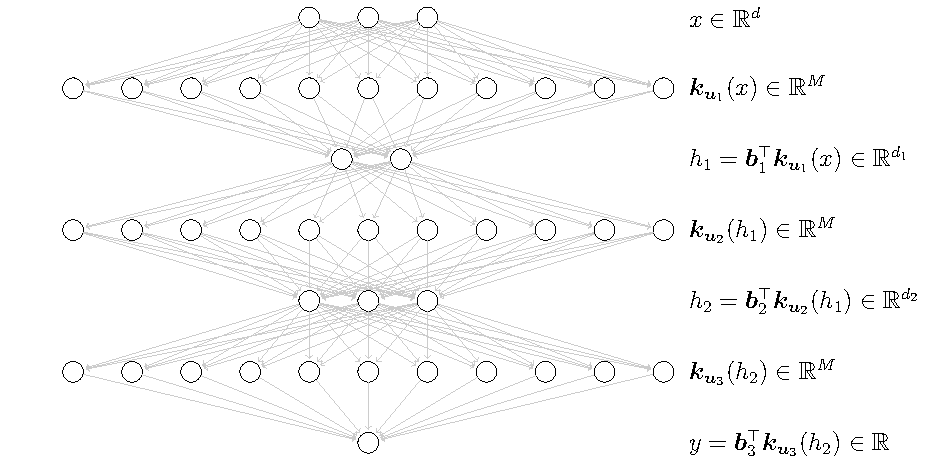
\includegraphics[width=\textwidth]{dgp_v2}
        \caption{Deep Gaussian process posterior}
        \label{fig:visual-dgp}
     \end{subfigure}
     \hfill
     \begin{subfigure}[b]{0.51\textwidth}
         \centering
        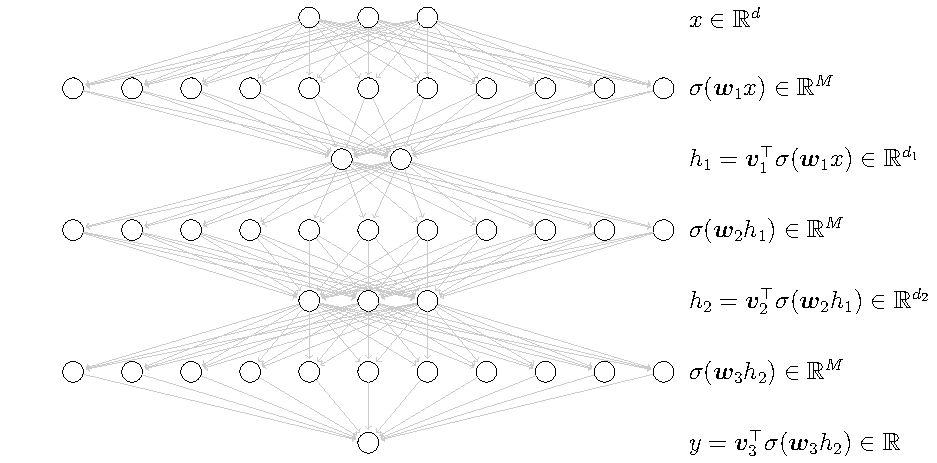
\includegraphics[width=\textwidth]{nn_v2}
         \caption{Fully-connected deep neural network}
         \label{fig:visual-nn}
     \end{subfigure}
    \caption{Forward pass through a DGP \textbf{(a)} and a DNN \textbf{b}. By matching basis functions $\kul(x)$ with $\sigma(\vw_\ell x)$ and weights $\bm{b}_\ell$ with $\bm{v}_\ell$ we obtain an equivalence between both models.} % Comparison between a DGP \textbf{(a)} and a DNN \textbf{(b)}. The goal is to design basis functions $\vc_{\vu}(\cdot)$ for the DGP that match to the activation functions $\sigma(\MW\,\cdot)$ used in the DNN.}
    \label{fig:visual}
\end{figure}

\subsection{Connection to Deep Neural Networks}
Investigating \cref{eq:qf-dgp}, it is worth noting that the posterior $q(f_\ell)$'s variance takes into account the infinite degrees of freedom from the prior; making predictions with an infinite amount of basis functions. The mean, on the contrary, has a finite numbers of parameters and can straightforwardly be re-written as a linear model with $M$ basis functions of the form $\kul(x) = \Cov(\vu_\ell, f_\ell(x))$:
\begin{equation}
    \label{eq:mean-qf}
    \Exp{f_\ell}{q(f_\ell(x))} = \bm{b}_\ell^\top \kul(x) \quad \text{where} \quad \bm{b}_\ell = \Kulul^{-1} \vm_\ell \in \Reals^M
\end{equation}
The mean of a layer in DGP is therefore ``not that different'' from a fully-connected layer in a neural network (NN-FCL), which admits the following structure
\begin{equation}
    \label{eq:fcn}
    \text{NN-FCL}_\ell(x) = \bm{v}_\ell\transpose \sigma(\bm{w}_\ell\,x),
\end{equation}
where $\sigma$ is the non-linear activations function (e.g., ReLU), $\bm{w}_\ell \in \Reals^{M \times d}$ and $\bm{v}_\ell \in \Reals^{M \times d_\ell}$ are the pre-activation and output weights, respectively. Looking at the resemblance between \cref{eq:mean-qf} and \cref{eq:fcn}, if we are able to formulate an inducing variable that makes the covariance $\kul(x)$ the same as a neural net activation function $\sigma(\bm{w}_\ell\,x)$, we will have a formal mathematical equivalence between the mean of GP layer in a DGP and a fully-connected neural network layer, that is $\ExpSymb[q(f_\ell(x))] = \text{NN-FCL}_\ell(x)$. By stacking many of these layers we obtain an equivalence between the forward pass in a DGP and a DNN, as visualised in \cref{fig:visual}.

In the next section we design the interdomain inducing variable for which the covariance will match the neural network activation function. This is the main contributions of this chapter. 


\section{Gaussian Process Layers with Activated Inducing Variables}
\label{sec:dnn-for-dgps:model}

Building on the exposition of zonal kernel RKHSs (\cref{sec:rkhs-dotproduct-kernels}) and interdomain inducing variables (\cref{section:interdomain-inducing-variables}) we can summarise our approach succinctly: we consider DGP models with GP layers that have an Arc Cosine kernel and Variational Fourier Feature style inducing variables $u_m = \langle f, {g}_m \rangle_\rkhs$ \citep{hensman2017variational}. In \cref{sec:inducing-function}, we then design inducing functions $g_m$ that have the same shape as neural network activation functions. Thanks to the reproducing property of the RKHS this yields basis functions $\kulx$ for the GP layers that correspond to activation functions (\cref{sec:relu-inducing-variables}), and thus to a DGP whose forward pass can be interpreted as a classic feed forward neural network. \Cref{sec:zonal-kernels-and-rkhs} covers the mathematical intricacies associated with the construction described above.

%%%%%%%%%%%%%%%%%%%%%%%%%%%%%%%%%%%%%%%%%%%%%%%%%%%%%%%%%%%%%%%%%%%%%%%%%
\subsection{Activated Inducing Functions}
\label{sec:inducing-function}

\paragraph{Preliminary: the bias term.}
We consider the RKHS of the first-order Arc Cosine kernel as discussed in \cref{sec:arccosine}, which consists of functions of the form $f(x) = \norm{x} g({x \over \norm{x}})$. As a result, all function in $\rkhs$ are equal to zero at the origin, i.e. $\forall f \in \rkhs: f({0}) = 0$, which is a very restrictive modelling assumption. To circumvent this problem we artificially increase the input space dimension by concatenating a constant to each input vector. In other words, the data space is embedded in a larger space with an offset such that it does not contain the origin anymore. This is analogous to the bias unit in multi-layer perceptron (MLP) layers in neural networks. For convenience we will denote by $(d-1)$ the dimension of the original data space (i.e. the number of input variables), and by $d$ the dimension of the extended space on which the Arc Cosine kernel is defined.

\begin{figure}[t]
    \centering
     \begin{subfigure}[b]{0.49\textwidth}
         \centering
        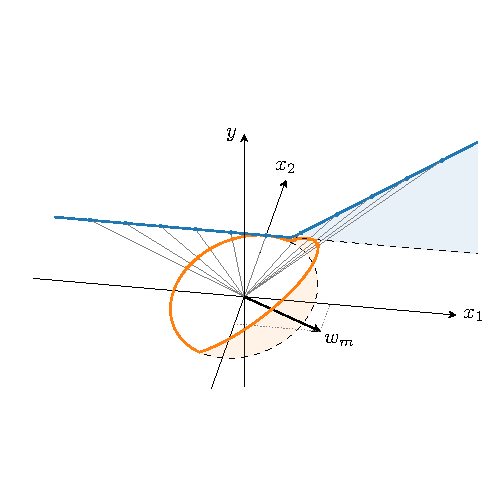
\includegraphics[clip, trim=0cm 1.8cm 0cm 1.6cm, width=\textwidth]{relu_mapping}
        %  \caption{$g_m(\vx) = \norm{\vw_m} \norm{\vx} \max\left(0, \frac{\vw_m^\top \vx}{\norm{\vw_m} \norm{\vx}}\right)$}
        \caption{ReLU: $\sigma(t) = \max(0, t)$}
         \label{fig:projection:relu}
     \end{subfigure}
     \hfill
     \begin{subfigure}[b]{0.49\textwidth}
         \centering
        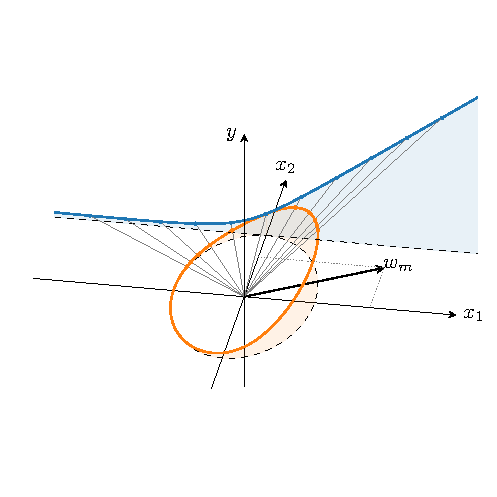
\includegraphics[clip, trim=0cm 1.8cm 0cm 1.6cm, width=\textwidth]{softplus_mapping}
        %  \caption{$g_m(\vx) = \norm{\vw_m}\norm{\vx} \left(\log(1 + \exp(\frac{3 \vw_m^\top \vx}{\norm{\vw_m} \norm{\vx}})) - c\right) $}
        \caption{Softplus: $\sigma(t) = \log(1 + \exp(3\,t))$}
         \label{fig:projection:softplus}
     \end{subfigure}
   \caption{Activated inducing function ${g}_m(x) = \norm{x}\,\norm{w_m}\, \sigma\left( w_m^\top x \, / \, \norm{w_m}\,\norm{x}\right)$ where $\sigma$ correspond to the ReLU \textbf{(a)} and Softplus \textbf{(b)}. Although the input domain is $\Reals^2$ we only plot the value of the function on the unit circle $\sphere^1$ (orange), and on the subspace that has an offset of $1$ in the $x_2$ direction (blue). The linear radial component of ${g}_m$ creates a one-to-one mapping between the blue curve and the upper half of the orange one.}%We observe that for these slices the functions correspond to the ReLU and Softplus neural network activation functions, respectively.}
   \label{fig:projection}
\end{figure}

\paragraph{Design of the inducing function.}
The inducing functions $g_m$ play an important role because they determine the shape of the SVGP's basis functions. Ideally they should be defined such that their restriction to the $(d - 1)$-dimensional original data space matches classic activation functions, such as the ReLU or the Softplus, exactly. However, this results in an angular component for $g_m$ that is not necessarily zonal. Since this property will be important later on, we favour the following alternative definition that enforces zonality:
\begin{equation}
\label{eq:def-inducing-function}
    g_m: \Reals^d \rightarrow \Reals,\qquad x \mapsto \norm{x}\,\norm{w_m}\, \sigma\left(\frac{w_m^\top x}{\norm{w_m}\,\norm{x}}\right), 
\end{equation}
with $w_m \in \Reals^d$ a parameter, and $\sigma: [-1, 1] \rightarrow \Reals$ the function that determines the value of $g_m$ on the unit hypersphere. In \cref{fig:projection}, we show that choosing $\sigma$ to be a ReLU ($\sigma(t) = \max(0, t)$) or a Softplus ($\sigma(t) = \log(1 + \exp(3\,t))$) activation function leads to inducing functions that closely resemble the classic ReLU and Softplus on the data space. In the specific case of the ReLU it can actually be shown that the match is exact. In both cases, the parameter $w_m \in \Reals^d$ determines the orientation and slope of the activation function---they play the same role as the pre-activation weights in a NN.

The zonality that we enforced in \cref{eq:def-inducing-function} is particularly convenient when it comes to representing $g_m$ in the basis of the eigenfunctions of $\rkhs$, which is required for computing inner products. It indeed allows us to make use of the Funk-Hecke theorem (see \cref{appendix:theorem:funk2}) and to obtain
\begin{equation}
\begin{aligned}
\label{eq:fourier-decomposition-activation-functions-new}
    g_m(x) = \norm{x}\, \norm{w_m} \sum_{n=0}^\infty &\sum_{j=1}^{\dnumharmonicsforlevel}  \sigma_n \phi_{n, j}\left(\frac{w_m}{\norm{w_m}}\right)\, \phi_{n, j}\left(\frac{x}{\norm{x}}\right), \\
   & \text{where \quad} \sigma_{n} = 
   \frac{\omega_{d}}{C_n^{(\alpha)}(1)} \int_{-1}^1 \sigma(t)\,C_n^{(\alpha)}(t)\,(1 - t^2)^{\frac{d-3}{2}} \calcd{t}.
\end{aligned}
\end{equation}
Analytical expressions for $\sigma_n$ when $\sigma(t)=\max(0, t)$ are given in \cref{app:sec:compute-eigenvalues}.

% [Representing functions on the sphere as a truncated series \cref{fig:activation-functions}]




\subsection{Activated Interdomain Inducing Variables}
\label{sec:relu-inducing-variables}

We define our \emph{activated} interdomain inducing variables as
\begin{equation}
\label{eq:def-inducing-variable}
    u_m = \big\langle f, {g}_m \big\rangle_\rkhs.
\end{equation}
Since the GP samples do not belong to the RKHS there are mathematical subtleties associated with such a definition, which are detailed in \cref{sec:zonal-kernels-and-rkhs}. Assuming for now that they are indeed well defined, using these interdomain inducing variables as part of the SVGP framework requires access to two quantities: (i) their pairwise covariance, and (ii) the covariance between the GP and the inducing variables. The pairwise covariance, which is needed to populate $\Kuu$, is given by
\begin{align}
\label{eq:kuu}
\Cov(u_{m}, u_{m'})  
&= \Cov \left( \big\langle f, {g}_m \big\rangle_\rkhs, \big\langle f, {g}_{m'} \big\rangle_\rkhs \right) \nonumber && \text{Definition $u_m$} \\
&= \langle {g}_m, {g}_{m'} \rangle_\rkhs \nonumber && \text{Definition RKHS} \\
&= \sum_{{n=0}}^{\infty} \sum_{j=1}^{\dnumharmonicsforlevel} \frac{\sigma_n \phi_{n,j}({w_m / \norm{w_m}}) \sigma_n \phi_{n,j}({w_{m'} / \norm{w_{m'}}})}{\lambda_n} \nonumber && \text{Fourier coefficients from \cref{eq:fourier-decomposition-activation-functions-new}} \\
&= \sum_{{n=0}}^{\infty}
    \frac{\sigma_n^2}{\lambda_n}\,\frac{n + \alpha}{\alpha}\,C_n^{(\alpha)}\left(\frac{w_m^\top w_{m'}}{\norm{w_m}\,\norm{w_{m'}}}\right) && \text{Addition \cref{theorem:addition}}.
\end{align}
Secondly, the covariance between the GP and $u_m$, which determines $[k_u(x)]_m$, is given by:
\begin{equation}
\label{eq:kuf}
  \Cov(u_m, f(x)) = 
    % \Cov(u_m, f(\cdot)) = % \Exp{f}{f(\vx) \langle f(\cdot), g_m(\cdot) \rangle_\rkhs} = 
    \langle k(x, \cdot), {g}_m \rangle_\rkhs = {g}_m(x) 
    % = \norm{\vw_m} \norm{\vx} \sum_{n=0}^{\tilde{N}} \sigma_n \frac{n + \alpha}{\alpha}\,C_n^{(\alpha)}(\frac{\vw_m^\top \vx}{\norm{\vw_m} \norm{\vx}}).
\end{equation}
as a result of the reproducing property of the RKHS. It becomes clear that this procedure gives rise to basis functions $\kux$ that are equal to our inducing functions $g_m$. By construction, these inducing functions match neural network activation functions in the data plane, as shown in \cref{fig:projection}. Returning to \cref{eq:mean-qf}, we see that using these inducing variables thus leads to an approximate posterior GP (\cref{eq:qf}) which has a mean that is equivalent to a fully-connected layer with a non-linear activation function (e.g.~ReLU, Softplus, Swish). 


%%%%%%%%%%%%%%%%%%%%%%%%%%%%%%%%%%%%%%%%%%%%%%%%%%%%%%%%%%%%%%%%%%%%%%%%%
\subsection{Analysis of the interplay between kernels and inducing functions}
\label{sec:zonal-kernels-and-rkhs}

In this section we describe the mathematical pitfalls that can be encountered \citep[e.g.,][]{sun2021neural} when defining new inducing variables of the form of \cref{eq:def-inducing-variable}, and how we address them. We discuss two problems: 1) the GP and the inducing function are not part of the RKHS, 2) the inducing functions are not expressive enough to explain the prior. Both problems manifest themselves in an approximation that is overly smooth and over-estimates the predictive variance.

\begin{figure}[t]
    \centering
    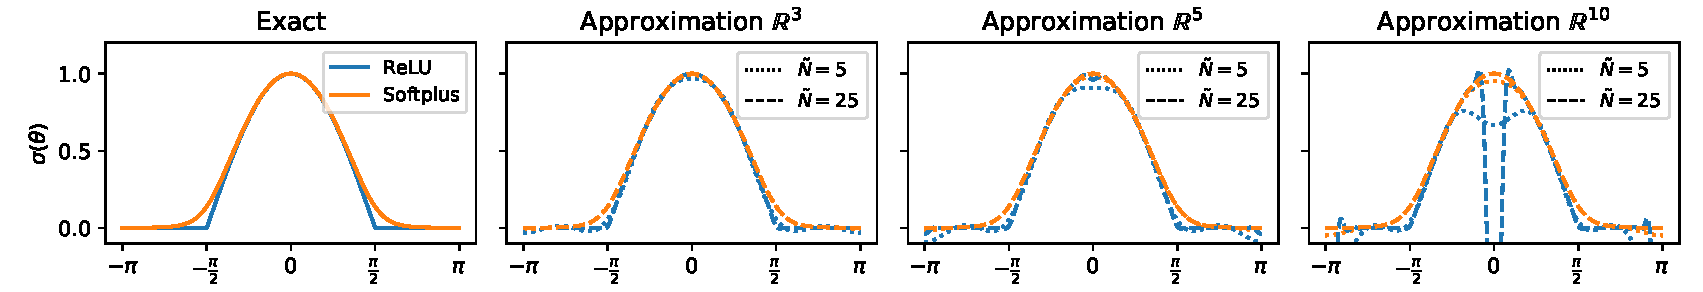
\includegraphics[width=\linewidth]{truncation_activations_circle}
    \caption{The exact ReLU and Softplus activation function and its approximation for different truncation levels and dimensions. These functions correspond to the orange function in \cref{fig:projection} plotted on a line rather than on the circle.}
    \label{fig:activation-functions}
\end{figure}

The Mercer representation of the kernel given in \cref{eq:mercer} implies that we have direct access to the Karhunen–Lo\`eve representation of the GP:
\begin{equation}
\label{eq:karhunen-loeve-2}
    f(x) =  \sum_{n=0}^\infty \sum_{j=1}^{\dnumharmonicsforlevel}  \xi_{n,j} \sqrt{\lambda_n} \norm{x} \phi_{n, j}\left(\frac{x}{\norm{x}}\right), \text{\quad where the } \xi_{n,j} \text{ are i.i.d. } \mathcal{N}(0, 1).
\end{equation}
Using this expression to compute the RKHS norm of a GP sample $f$ yields $\norm{f}^2 = \sum_{n, j} \xi_{n,j}^2$, which is a diverging series. This is a clear indication that the GP samples do not belong to the RKHS \citep{kanagawa2018gaussian}, and that expressions such as $\langle f, g \rangle_{\rkhs}$ should be manipulated with care. By definition, the RKHS inner product is a series that converges if computed for any two elements  $g, h \in \rkhs$. The inner product operator can, however, be extended to the case where one input lives in a space larger than $\rkhs$, provided that restrictions are introduced on the second input to guarantee the convergence of the series. In other words, even if the decay of the Fourier coefficients of $f$ is too slow to make it an element of \rkhs, if the Fourier coefficients of $g$ decay quickly enough for the series $\sum_{n,j} \xi_{n,j} g_{n,j}/ \sqrt{\lambda_n}$ to converge then $\langle f, g \rangle_{\rkhs}$ is well defined.
%Though the theoretical setup in the previous paragraphs gives us an equivalence between a fully-connected neural network layer with a non-linear activation and the mean of an approximate SVGP, we need to proceed with caution to make sure that our method is mathematically sound, and practically useful. Indeed, since the GP samples do not belong to the RKHS, there are mathematical subtleties associated with manipulating expressions such as $\langle f(\cdot), g_m(\cdot) \rangle_{\rkhs}$ and attention must be paid to ensure this expression is meaningful. This is sometimes overlooked and can result in inducing variables with limited expressiveness, as it is the case in \citet{sun2021neural}.

%For the definition of the inducing variable (see~\cref{eq:fourier-decomposition-activation-functions-new}) to be valid a necessary condition is that $f(\cdot)$ and $g_m(\cdot)$ are both part of the RKHS. We already know that a GP sample does not belong to the RKHS \citep{kanagawa2018gaussian}, and, while we managed to write $g_m(\cdot)$ as a linear combination of the basis functions $\sh_{n, j}(\cdot)$ in \cref{eq:fourier-decomposition-activation-functions-new}, this does not guarantee its presence in $\rkhs$. This makes our inducing variables definition questionable. For the ReLU inducing function (i.e. $g_m(\cdot)$ with $\sigma(t) = \max(0,t)$ as in \cref{fig:projection:relu}), this concern is justified. Through the decay rate of $\sigma_n$, which is proportional to the square root of those of the corresponding Arc Cosine \citep{bach2017breaking,bietti2020deep}, it is easy to see that $\norm{g_m(\cdot)}_{\rkhs} > \infty$. This means that the ReLU inducing functions are not part of the first-order Arc Cosine RKHS ---reflecting the discontinuous nature of the function. Fortunately, by using smoother activation functions for $\sigma(t)$ (e.g.,~Softplus), for which the coefficients $\sigma_n$ decay faster than the eigenvalues of the kernel, the norm can be made finite and the activated inducing function part of the RKHS.

The above reasoning indicates that, for a given kernel $k$, some activation functions $g_m$ will result in inducing variables $u_m = \langle f, g_m \rangle_{\rkhs}$ that are well defined whereas other activation functions do not. For example, if we consider the case of the Arc Cosine kernel and the ReLU inducing function, the decay rate of $\sigma_n$ is proportional to the square root of $\lambda_n$~\citep{bach2017breaking,bietti2020deep}. This implies that the inner product series diverges and that this kernel and inducing variable cannot be used together. Alternatively, using smoother activation functions for $\sigma(t)$, such as the Softplus, results in a faster decay of the coefficients $\sigma_n$ and can guarantee that inducing variables are well defined. We notice this behaviour in the bottom plots of \cref{fig:trunc}, where the norm $\norm{g_m}$ in the case of the ReLU (left) keep growing with $N$, whereas the norm for the softplus converges. This will have implications on the GP fit, as later discussed.

An alternative to ensure the series convergence for any combination of kernel and activation function is to use a truncated approximation of the activation function $\tilde{g}_m$ where all the Fourier coefficients above a given level $\tilde N$ are set to zero, which basically turns the inner product series into a finite sum. % Making use of the addition theorem (see \cref{app:sec:harmonics}), this yields:
% \begin{equation}
%     \tilde{g}_m(\vx) = \norm{\vw_m} \norm{\vx} \sum_{n=0}^{\tilde{N}} \sigma_n \frac{n + \alpha}{\alpha}\,C_n^{(\alpha)}(\frac{\vw_m^\top \vx}{\norm{\vw_m} \norm{\vx}}).
% \end{equation}
\Cref{fig:activation-functions} shows how the true and truncated activation functions for the ReLU and Softplus compare. These correspond to the orange functions in \cref{fig:projection}, but are now plotted on a line. In the low to medium dimensional regime, we see that even for small truncation levels we approximate the ReLU and Softplus well. In higher dimensions this becomes more challenging for the ReLU. % and we notice high frequency variations near the boundary that are reminiscent of the Gibbs phenomenon in Fourier analysis. 

\paragraph{Inexpressive inducing variables through truncation (\cref{fig:trunc})} The main concern with this truncation approach, however, comes from elsewhere: the larger $\tilde N$ is, the closer $\tilde{g}_m$ is to $g_m$, but the larger $\norm{\tilde{g}_m}_{\rkhs}$ becomes (to the point where it may be arbitrarily large). Similarly to ridge regression where the norm acts as a regulariser, using inducing functions with a large norm in SVGP models comes with a penalty which enforces more smoothness in the approximate posterior and limits its expressiveness.
\Cref{fig:trunc} shows how the norm of our ReLU inducing functions grow in the RKHS. So by making $\tilde{N}$ larger such that we approximate the ReLU better, we incur a greater penalty in the ELBO for using them. This leads to unexpressive inducing variables, which can be seen by the growing predictive uncertainty. The Softplus, which is part of the RKHS, does not suffer from this.

\begin{figure}[t]
\centering
\begin{minipage}{.48\textwidth}
  \centering
  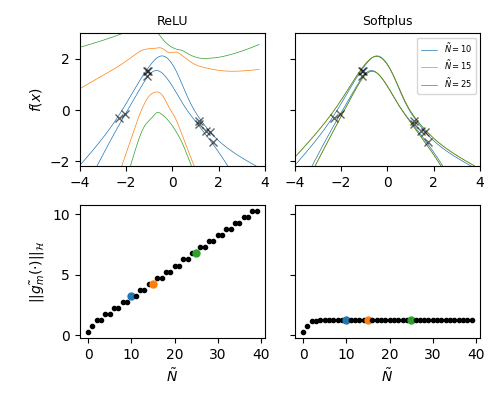
\includegraphics[width=\linewidth]{truncation_colors}
  \captionof{figure}{\textbf{Top:} Predictive variance an SVGP fit on a synthetic dataset using our ReLU (left) and Softplus (right) inducing variables for $\tilde{N}={\color{C0}10}, {\color{C1}15}$ and ${\color{C3}25}$. \textbf{Bottom:} the norm of the inducing function $\tilde{g}_m$ as a function of $\tilde{N}$.}
  \label{fig:trunc}
\end{minipage}\hfill
\begin{minipage}{.48\textwidth}
  \centering
  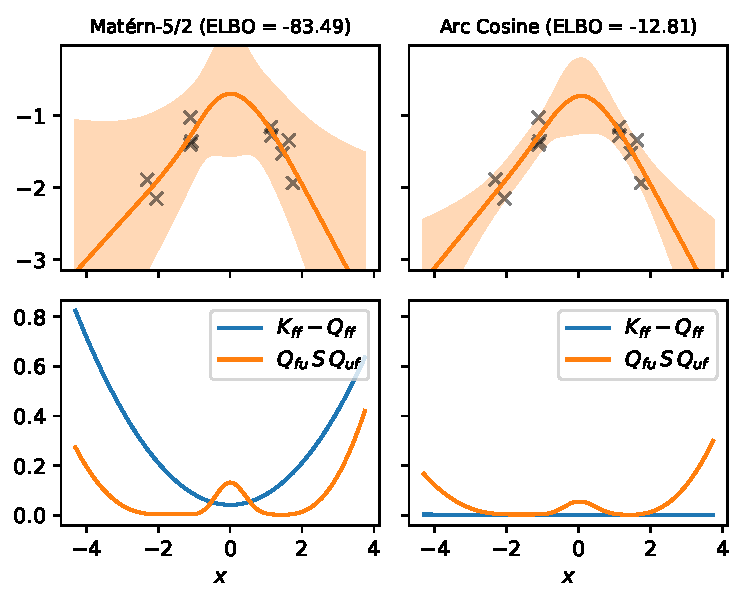
\includegraphics[width=\linewidth]{fits_and_variance_mat52_arccosine}
  \captionof{figure}{\textbf{Top:} Predictive mean and variance for an SVGP model using our Softplus inducing variables for the Mat\'ern-5/2 (left) and Arc Cosine (right) kernel. \textbf{Bottom:} The two terms that constitute the predictive variance.}
  \label{fig:matern-vs-arccosine}
\end{minipage}
\end{figure}

\paragraph{Inexpressive inducing variables through spectra mismatch (\cref{fig:matern-vs-arccosine})} Any stationary kernel whose inputs $\vx,\vx' \in \dsphere$ are restricted to the unit hypersphere is a zonal kernel (i.e., the kernel only depends on the dot-product). This means that we are not limited to only the Arc Cosine kernel because we can replace the shape function in \cref{eq:arccosine} by any stationary kernel, and our approach would still hold. For example, we could transform the Mat\'ern-5/2 to a zonal kernel as follows
\begin{equation*}
    k(x, x') = \norm{x} \norm{x'} \kappa_{\text{mat-5/2}}\Big(\frac{x^\top x'}{\norm{x}\norm{x'}}\Big),\ \text{with}\ \kappa_{\text{mat-5/2}}(t) = \gamma ^{2}\left(1+{\frac {{\sqrt {5}} t}{\rho }}+{\frac {5 t^{2}}{3\rho ^{2}}}\right)\exp \left(-{\frac {{\sqrt {5}} t}{\rho }}\right),
\end{equation*}
$\gamma^2$ is the variance and $\rho$ the lengthscale. However, in \cref{fig:matern-vs-arccosine} we compare the fit of an SVGP model using a Mat\'ern-5/2 kernel (left) to a model using an Arc Cosine kernel (right). While both models use our Softplus inducing variables, we clearly observe that the Mat\'ern kernel gives rise to a worse posterior model (lower ELBO and an over-estimation of the variance). In what follows we explain why this is the case.

\begin{figure}[t]
    \centering
    \includegraphics[width=\linewidth]{spectra_kernels_and_activations.pdf}
    \caption{Spectra of Arc Cosine and Mat\'ern-5/2 (blue), and ReLU and Softplus (orange) for different levels.}
    \label{fig:spectra}
\end{figure}

In the bottom panel in \cref{fig:matern-vs-arccosine} we see that for the Mat\'ern-5/2, the Nystr\"om approximation $\Qff = \Kfu \Kuu^{-1} \Kfu^\top$ is unable to explain the prior $\Kff$, imposed by the kernel. This leads to the overestimation of the predictive variance in the top plot. The reason for this problem is the mismatch between the eigenvalues $\lambda_n$ (\cref{eq:compute-fourier-coefficients}) of the Mat\'ern and the Fourier coefficients $\sigma_n$ (\cref{eq:fourier-decomposition-activation-functions-new}) of the Softplus inducing function. As shown in \cref{fig:spectra}, the Mat\'ern kernel has a full spectrum (i.e., $\lambda_n \neq 0,\ \forall n \in \Naturals$), whereas the coefficients for the Softplus $\sigma_n$ are zero at levels $n=3, 5, 7,\cdots$. We are thus trying to approximate our prior kernel, containing all levels, by a set of functions that is missing many. This problem does not occur for the combination of Softplus (or ReLU) inducing functions and the Arc Cosine kernel (right-hand side) because their spectral decomposition match. In other words, the Arc Cosine kernel has zero coefficients for the same levels as our activated inducing functions. 

Taking the above two cases into consideration which lead to inexpressive inducing variables, in the upcoming experiments we use the Arc Cosine kernel and inducing variables obtained with the Softplus activation (\cref{sec:inducing-function}) with $\tilde{N} = 20$.

%%%%%%%%%%%%%%%%%%%%%%%%%%%%%%%%%%%%%%%%%%%%%%%%%%%%%%%%%%%%%%%%%%%%%% Experiments

\section{Experiments}
\label{section:dnn-for-dgps:experiments}

We have shown that that we can build SVGP models with basis functions that behave like neural net activations. This equivalence has the practical advantage that we can train the means of the GP layers in our DGP as if they are a neural network model --- making use of the great advances made by the deep learning community. Once the mean of the DGP is trained, we can further optimise the remaining model hyper- and variational parameters w.r.t. the ELBO, which is a more principled objective \citep{Fong2019On}. This approach allows us to exploit the benefit of both, the efficient training of the DNN in combination with the principled uncertainty estimate of the DGP. 

The aim of the experiments is to highlight that (i) our method leads to valid inducing variables, (ii) our initialisation improves DGPs in terms of accuracy, and (iii) we are able to improve on Dropout-based \citep{Gal2016dropout} neural networks in terms of calibrated uncertainty. 
%We show this on a wide range of problems.
We acknowledge that the NNs we benchmark against are the models for which we can build an equivalent DGP. While this leads to a fair comparison, it excludes recent improvements such as Transformer and Batch Norm layers.


% \begin{figure}[t]
%     \centering
%     \includegraphics[width=\linewidth]{figures/banana-M-ELBO.pdf}
%     \caption{Fits on the Banana binary classification dataset with growing number of inducing variables $M$. \textbf{left three panels:} In blue and orange we display the data. The model's $p(y \given \vx)$ is given as shades of grey. \textbf{right panel:} ELBO as a function of the number of inducing variables.}
%     \label{fig:banana}
% \end{figure}

% \paragraph{2D classification on Banana dataset} An attractive property of SVGPs (and DGPs) is that the objective is a lower bound on the log marginal likelihood, where the gap is the KL divergence between the true and approximate posterior. By increasing the number of inducing variables we make the approximate posterior richer, lowering the error, or equivalently, tighten the bound. In \cref{fig:banana} we verify this property for a single-layer SVGP model with our Softplus activated inducing variables and an Arc Cosine kernel. Given the small dataset size, we optimised the model's parameter using BFGS. This experiment validates that we designed valid inducing variables and that, as theory suggest, the ELBO improves with number of inducing variables.

% \begin{figure}[t]
%     \centering
%     \includegraphics[width=\linewidth]{figures/bananafull.pdf}
%     \caption{We compare the fit of a single-layer and three-layer DNN optimised using binary cross-entropy and it's equivalent DGP trained using the ELBO. The DNNs are very confident, even far away from the data. We used the DNNs to initialise the equivalent DGP posterior mean before optimising the ELBO, which in both situations leads to a model exhibiting more calibrated uncertainty.}
%     \label{fig:deep-banana}
% \end{figure}

% \paragraph{From Neural Network to Activated DGP} \Cref{fig:deep-banana} shows the difference in predictive probability $p(y \given \vx)$ for a DNN and our activated DGP, in the single-layer and three-layer case. We configure the models with a Softplus activation function and set the number of both inducing variables of the GP and hidden units of the DNN to 100. In this experiment, the first step is to optimise the DNN w.r.t. the binary cross-entropy objective, upon convergence we initialise the DGP with this solution and resume training of the DGP w.r.t. the ELBO. Especially in the single-layer case, we notice how the sharp edges from the NN are relaxed by the GP fit, and we see how the GP expresses uncertainty away from the data by letting $p(y \given \vx) \approx 0.5$. This is thanks to the ELBO, which balances both data fit and model complexity and simultaneously trains the uncertainty.

\subsection{Regression on UCI benchmarks}
We compare a suit of models on a range of regression problems. The important aspect is that we keep the model configuration and training procedure fixed across datasets. We use three-layered models with 128 inducing variables or hidden units. In each layer, the number of output heads is equal to the input dimensionality of the data. The Activated DGP (ADGP) and neural network approaches (Vanilla and Dropout) use Softplus activation functions. The Dropout model~\citep{Gal2016dropout} uses a rate of $0.1$ during train and test, and the Vanilla model is a deterministic neural network that uses the training MSE as the empirical variance during prediction.

The DGP and ADGP both use the Arc Cosine kernel. The main difference is that the DGP has standard inducing points $u_m = f(z_m)$, whereas ADGP makes use of our activated inducing variables $u_m = \langle f, g_m \rangle_\rkhs^{}$. The ADGP is trained in two steps: we first train the mean of the approximate posterior w.r.t. the MSE, and then optimise all parameters w.r.t. the ELBO.

In \cref{fig:uci} we see that in general our ADGP model is more accurate than its neural network initialisation (Vanilla model) in terms of RMSE. This is a result of the second stage of training in which we use the ELBO rather than the MSE, which is especially beneficial to prevent overfitting on the smaller datasets. When it comes to NLPD, ADGP shows improvements over its NN initialisation for 5 datasets out of 7 and consistently outperforms classic DGPs.

\begin{figure}
    \centering
    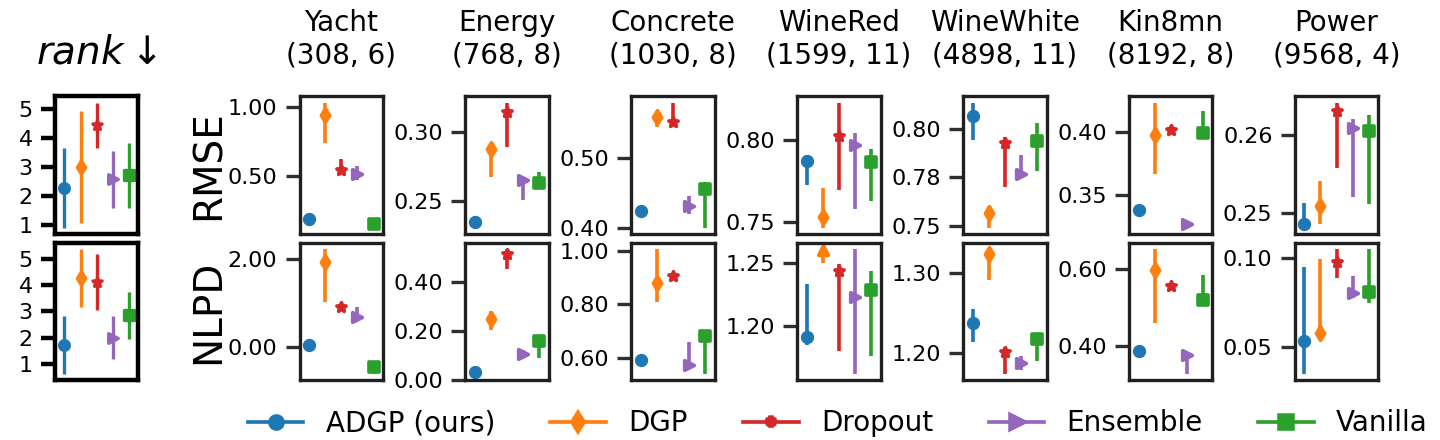
\includegraphics[width=\textwidth]{uci_small}
    \caption{UCI: Root Mean Squared Error (RMSE) and Negative Log Predictive Density (NLPD) with 25\% and 75\% quantile error bars based on 5 splits. Dataset size and dimension given in parentheses.}
    \label{fig:uci}
\end{figure}

\subsection{Large scale image classification}
% \label{sec:experiment:classification}
In this experiment we measure the performance of our models under dataset shifts \citep{Ovadia2019}. For MNIST and Fashion-MNIST the out-of-distribution (OOD) test sets consist of rotated digits --- from 0\textdegree (i.e. the original test set) to 180\textdegree. For CIFAR-10 we apply four different types of corruption to the test images with increasing intensity levels from 0 to 5. For MNIST and FASHION-MNIST the models consist of two convolutional and max-pooling layers, followed by two dense layers with 128 units and 10 output heads. The dense layers are either fully-connected neural network layers using a Softplus activation function (Vanilla and Dropout), or our Activated GP layers using the Arc Cosine kernel and Softplus inducing variables (ADGP). For the CIFAR-10 models, we use the residual convolutional layers from a ResNet~\citep{he2016deep} to extract useful features before passing them to our dense GP or NN layers. As previously, the ADGP model is initialised to the solution of the Vanilla model, and training is then continued using the ELBO. In \cref{fig:image-classification} we observe that the models perform very similar in terms of prediction accuracy, but that ADGP better account for uncertainty as evidenced by the Test Log Likelihood metric.% (TLL) we see that the ADGP outperforms the NN approaches by quite a margin.

\begin{figure}[t]
    \centering   
    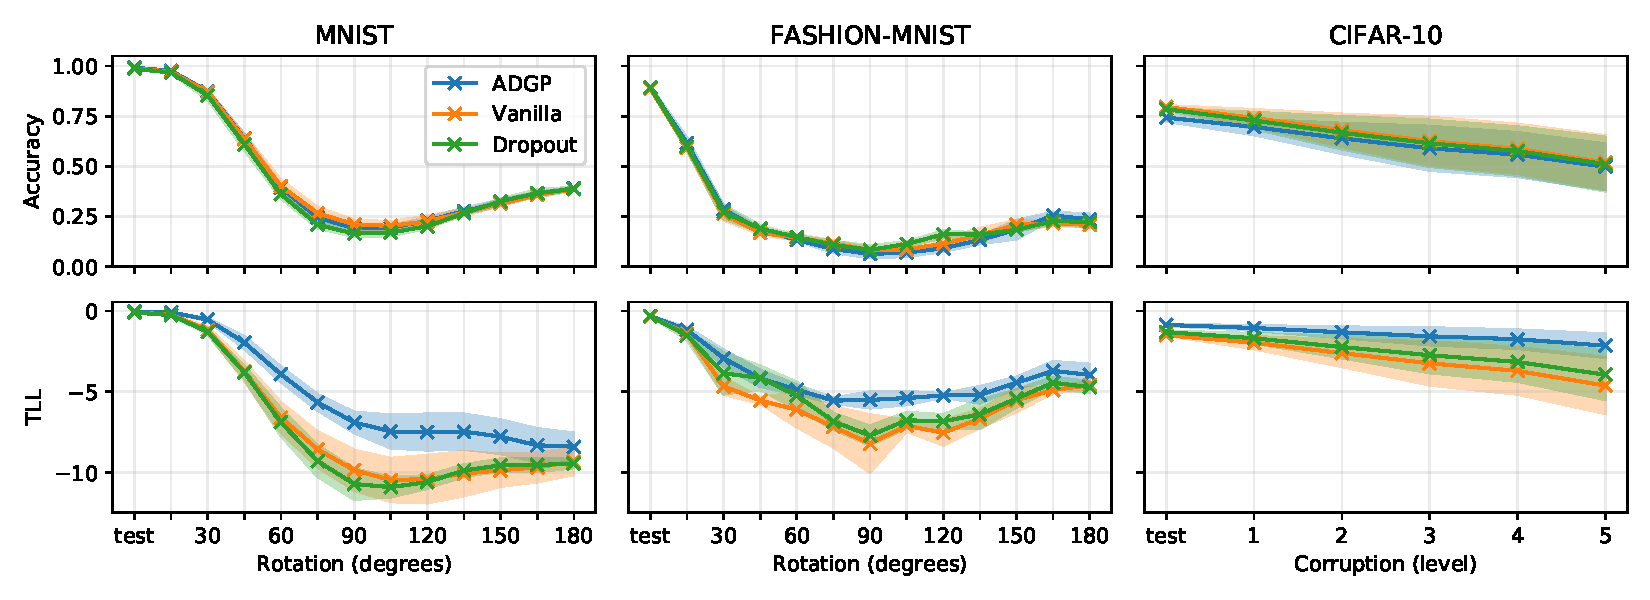
\includegraphics[width=\textwidth]{image_classification}
    \caption{Results on the rotated MNIST, FASHION-MNIST and corrupted CIFAR-10, showing the mean and std. dev. of the accuracy \textbf{(top)}, and test log-likelihood (TLL) \textbf{(bottom)}.}
    \label{fig:image-classification}
\end{figure}


\section{Conclusion}

In this chapter, we establish a connection between fully-connected neural networks and the posterior of deep sparse Gaussian processes. We use a specific flavour of interdomain inducing variables based on the RKHS inner product to obtain basis functions for the SVGP that match activation functions from the neural network literature. By composing such SVGPs together, we obtain a DGP for which a forward pass through the mean of each layer is equivalent to a forward pass in a DNN. We also address important mathematical subtleties to ensure the validity of the approach and to gain insights on how to choose the activation function. 

\graphicspath{{Chapter5/Figs/}}

\chapter{Future Research Agenda}
\label{chapter:future-research}

\section{Introduction}
To date, my research has focussed on using Gaussian processes (GPs) as building blocks for deep models, similar to neural network layers. In this vein, I have worked on (1) deep convolutional Gaussian processes that mimic the convolutional and layered architectures encountered in many contempory deep learning models \citep{Dutordoir2020convolutional}, (2) conditional density estimation models which are similar to Variational Auto Encoders \citep{dutordoir2018cde,Salimbeni2019}, and (3) more recently, deep Gaussian processes that have basis functions that are similar to neural network activation functions \citep{dutordoir2021deep} (discussed at length in \cref{chapter:dnn-as-point-estimate-for-dgps}). I have packaged these advances in a software toolbox, called GPflux \citep{dutordoir2021gpflux}, which provides these GP layers through a neural network like interface. The main advantage of this approach is that straightforward application of Bayesian principles leads to sensible results, which is not necissarily the case for normal neural networks \citep{wenzel2020good}. The current state of research into using Gaussian processes as layers is that classification performance starting to be on-par with deep learning on simple datasets \citep{dutordoir2018cde}, but with good uncertainty quantification and automatic selection of hyperparameters working `out of the box'.

The primary focus of my previous research can be considered as `curve-fitting', i.e. finding the best function approximator when given examples of inputs and corresonponding outputs. In this setting we can consider two regimes: (1) the function is very complex but there is an abundance of high-quality and cheap data to learn the mapping, and (2) the function is of a simpler nature but the underlying data is limited, noisy and/or very expensive to acquire. As evidenced by many recent advances in domains such as natural language and vision, where indeed there is a large availablility of high-quality data, the first regime is a setting where deep learning thrives. The natural inductive bias of deep neural networks (DNNs) in combination with the low computational cost of training them on massive datasets has proven to be very effective. Arguably, performing (approximate) Bayesian inference in this regime will contribute little to the end result, and the computational cost associated with it makes it very cumbersome. 

The second regime, in which data is noisy, requires a completely different modelling paradigm. On the one hand, the noisy data forces the model to be uncertain about the signal that can be extracted from the given examples. On the other hand, the simpler nature of the function allows an expert to encode prior information about the problem at hand. This enables faster generalisation from little data, which can be necessary given the high cost of acquiring more. This is a setting where probabilistic Bayesian models thrive.

However, to fully valorise Bayesian models one needs to consider them as part of a larger `decision-making' system. In these systems probabilistic models can be used to determine optimal actions to take in order to achieve a certain outcome. % For example, finding the input value that minimises an unknown `black-box' function. % Since good decisions depend on the confidence of our knowledge, faithfully representing uncertainty is a crucial aspect of the models.

In the next chapter of my PhD, I want to evolve from purely `curve-fitting' applications to focusing more on decision-making systems that \emph{use} probabilistic models to drive their decisions. In particular, I want to focus on probabilistic models that take into account the geometry of the problem at hand. This will allow encorporating more accurately physical properties and constraints of the system under study. In the next section we briefly discuss Markov Decision Processes (MDPs), a formal mathematical framework to decision making. We pay attention to the model based approach. InSection we can define probabilistic models in non-Euclidian spaces. on  . We finish with suggesting concrete research topics and a real-world application.

% . I would like to focus on both the modelling side and the decision-making aspect using the model's outputs. In the next two sections we discuss the type of decision system we consider and how we can define Gaussian processes on these spaces. 

\section{Markov Decision Process}

A discrete-time Markov decision Process (MDP) is a stochastic control process. It provides a mathematical framework for decision making in situations where outcomes are partly random and partly under the control of a decision maker [CITE TODO]. A MDP is characterised by a 4-tuple, consiting of
\begin{enumerate}
    \item A state space $\mathcal{S}$,
    \item An action space $\mathcal{A}$,
    \item Reward density $p(r \given a, s)$: the immediate reward obtained after executing an action $a$ in a given state $s$,
    \item Transition density $p(s' \given a, s)$: transitioning from state $s$ to state $s'$, due to action $a$.
\end{enumerate}
It should be noted that this is a very broad definition, yet there are still many variations to it. For instance, one can consider deterministic reward and transition functions, continuous-time and partially observed MDPs.

The objective of an MDP is to find a `good' (probabilistic) policy function $\pi:\mathcal{S} \rightarrow \mathcal{X}$. This is a mapping that specifies which action a decision maker should take in a given state $s$. The goal is to find a sequence of actions, starting from an initial state $s_0$, that maximses the cumulative reward a decision maker obtains by obeying the policy $\pi$. This is given by the value function
\begin{equation}
    V^{(\pi)}(s_0) = \Exp{}{\sum_t r_t}
\end{equation}
where the expectation is over $r_t \sim p(r_t \given s_t, a_t)$, $s_{t+1} \sim p(s_{t+1} \given s_t, a_t)$ and $a_t \sim \pi(s_t)$.

The quality of a policy $\pi$ is given by the \emph{regret}, which measures the value function $V^{(\pi)}$ relative to the optimal value function $V^{*}$ obtained by the best possible policy $\pi^*$
\begin{equation}
    R^{(\pi)}(s_0) = V^*(s_0) - V^{(\pi)}(s_0). 
\end{equation}

\subsection{A Model-based Approach}
There are many different ways to deduct a good---or even an optimal---policy for a given MDP, but the exact algorithm will heavily depend on the precise formulation of the problem. Here, we consider the case that the transition and reward function are unknown, and also very expensive to evaluate. In this setting, any efficient algorithm will need to consider whether to take explorative actions that might lead to better rewards, or take advantage of actions that are known to be good but will not improve the current solution. This dilema is known as the exploitation-exploration trade-off. The fact that the functions are expensive to evaluate makes it worthwile to spend resources (e.g., time and compute) on deciding where to evaluate them next.

A strategy to address this MDP formulation is using a \emph{model-based} approach. Broadly speaking, this approach consists of a model that learns the unknown transitions and/or rewards from observed data in a supervised learning way. Subsequently, a policy is derived using the learned model rather than using the true reward and transition functions. % The exploitation-exploration trade-off highlights the importance of the model to faitfully represent the uncertainty present in the data.

\paragraph{Example}
We consider Bayesian optimisation (BO) [CITE] as an illustration of these concepts. BO is a sequential search algorithm for finding a global minimiser of an unknown objective function $f$ defined over a domain of interest $\mathcal{X}$
\begin{equation}
    x_* = \argmin_{x \in \mathcal{X}} f(x).
\end{equation}
The function $f$ is not observed directly. Instead, at each step the algorithm selects a query point $x \in \mathcal{X}$ at which to evaluate $f$ and obtains $y(x)$: a function evaluation corrupted by noise $y(x) \sim p(y(x) \given f(x))$. 

BO can be framed as a MDP if one considers the cardinality of $\mathcal{S}$ to be $1$, and the actions space to cover the function's input domain $\mathcal{A} = \mathcal{X}$. As there is only a single state the transition functions trivially reduces to the identity function. The reward associated to an action $x$\footnote{To adhere to the common notation in BO we use $x$, rather than $a$, to represent the action (in our case the next query point).} is given by the negative function observation. This construction leads to an unknown and probabilistic reward  function due to the unknown objective function and the noisy observations. Collecting the sequence of actions (i.e. query points) $\{x_t\}$, the performance of an algoritm selecting the query points can be measured using a tailered notion of reget
\begin{equation}
    R = \sum_t f(x_t) - f(x_*).
\end{equation}

A model-based approach to this problem employs a surrogate model $g$ which learns the unknown objective function $f$ using past observations. The surrogate model is used to decide on the next query point, through what is known as an \emph{acquisition rule} [CITE]. The exploitation-exploration trade-off highlights the importance of the surrogate model's faithful represention of uncerainty about the objective. It is a key ingredient to an effective algorithm and is necessary to obtain a low regret [CITE]. Most model-based approaches employ Gaussian processes (GPs) as their surrogate model: $g \sim \GP$ [CITE]. 

To follow a model-based approach in Bayesian optimisation, as well as in other kinds of MDPs, it is required to define a GP on the domain of interest. For convenience, this domain is typically chosen to be the Euclidian space. However, many problems possess important non–Euclidean geometric structure, which makes it much more effective and convenient to directly specify the problem on the non-Euclidean domain, like the torus or the sphere, but also a graph, a rotation group, or the space of positive-definite matrices. Consider for example optimising the joint postures of a robot, which are defined on the torus $\mathcal{T}^d = \mathcal{S}^1 \times \mathcal{S}^1 \ldots \times \mathcal{S}^1$. To accomodate for this, one must be able to specify a GP prior, or equivalently define a kernel, on this space of interest.

\section{Gaussian Processes as Surrogate Models in non-Euclidian manifolds}

\begin{figure}[tbh!]
  \centering
\begin{subfigure}{0.3\textwidth}
  \vspace{.3cm}
  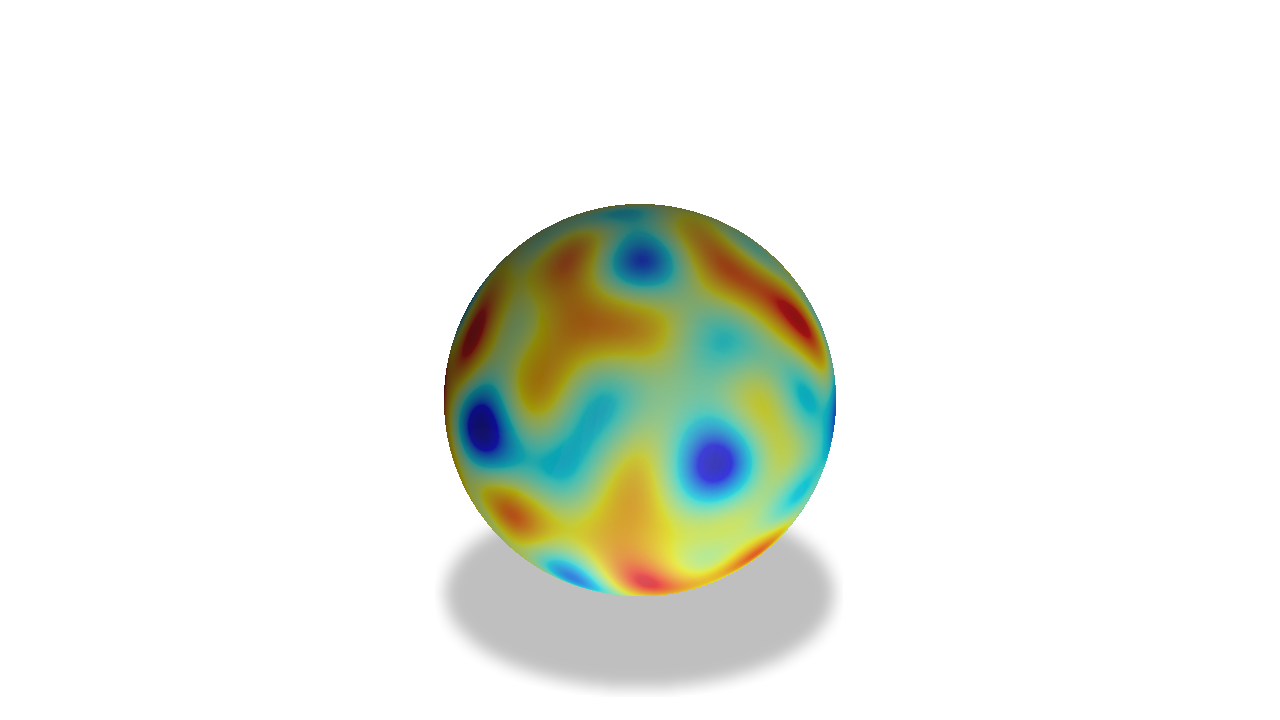
\includegraphics[clip, trim=12cm 0cm 12cm 7cm,width=\textwidth]{sphere}
  \caption{Sphere}
  \label{fig:sphere}
\end{subfigure}\hfil % <-- added
\begin{subfigure}{0.3\textwidth}
  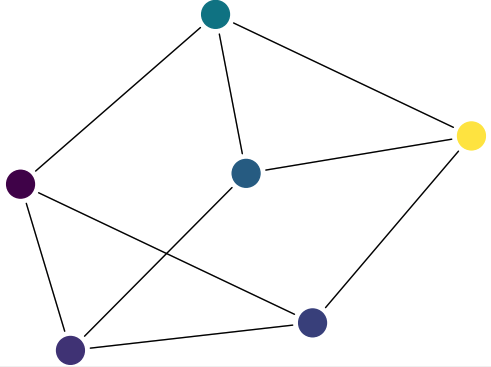
\includegraphics[clip, trim=0cm .05cm 0cm 0cm, width=\textwidth]{graph}
  \vspace{.5cm}
  \caption{Graph}
  \label{fig:graph}
\end{subfigure}\hfil % <-- added
\begin{subfigure}{0.3\textwidth}
  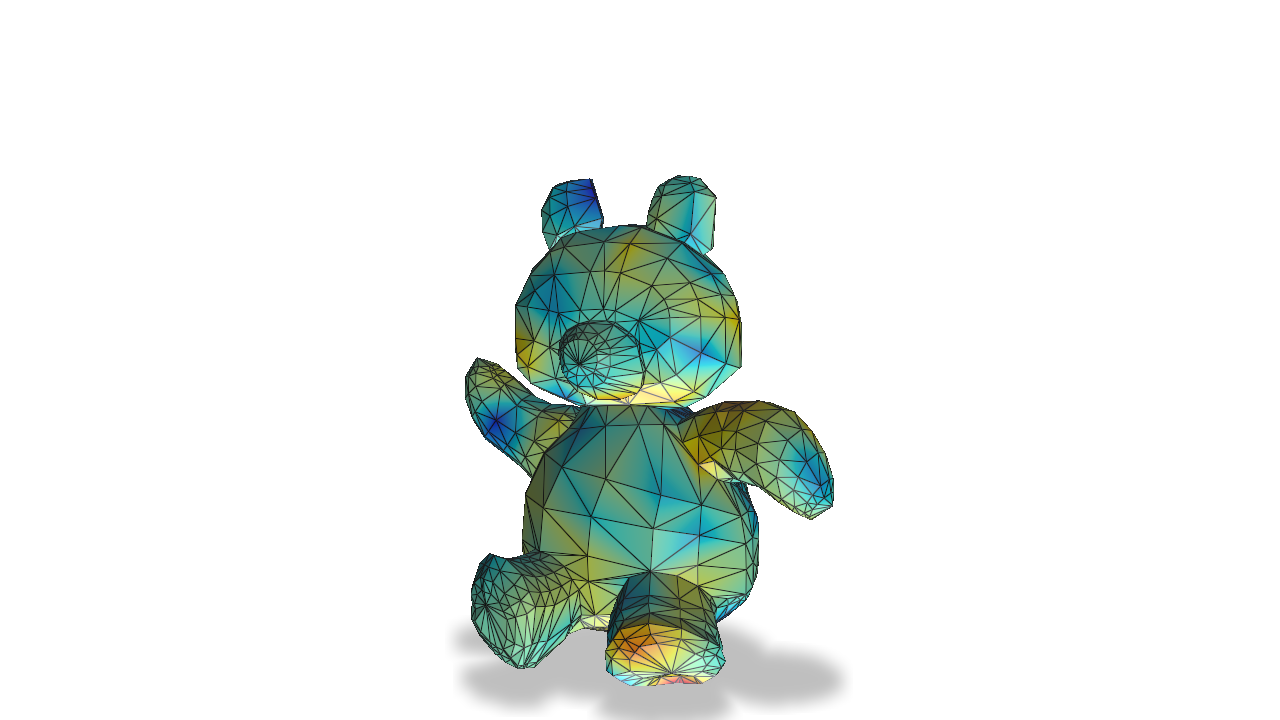
\includegraphics[clip, trim=12cm 0cm 12cm 5cm,width=\textwidth]{teddy_mesh}
  \caption{Mesh}
  \label{fig:mesh}
\end{subfigure}
\caption{Mat\'ern GP samples on non-Euclidian spaces}
\label{fig:xxxx}
\end{figure}

Stationary kernels are ubiquitous in Gaussian processes when the input space is Euclidean. Their popularity is due to their general useability and the ease of understanding which prior information they encode. Recent work of \citet{Borovitskiy2020} has extended the definition of stationary kernels to Riemannian manifolds. This enables the definition of symmetric and positive-definite kernels, which characterise GPs, that take into account the geometry of the space. In the case of a graph, for example, two nodes can be close to each other in the Euclidean space yet far apart in the term of number of edges them separates them. A classical statioary kernel is not able to capture this information, whereas a geometric aware kernel can.

The construction in \citet{Borovitskiy2020} relies on the spectral theory of the Laplace-Beltrami operator and defines the kernel through its Mercer decomposition (\cref{eq:mercer})
\begin{equation}
    \label{eq:borovitskiy}
    k(x, x) = \sum_i S(\sqrt{\lambda_i})\,\phi_i(x)\,\phi_i(x')
\end{equation}
where $S$ is the power spectrum of the kernel and $\{\lambda_i, \phi_i\}$ are the eigenvalues and eigenfunctions of the Laplace-Beltrami operator. \cref{chapter:vish} discusses a special case of this construction for zonal kernels defined on the hypersphere where the eigenfunctions are given by the spherical harmonics.

The elegance of \cref{eq:borovitskiy} is that it defines the kernel through the eigenfunctions of the Laplace-Beltrami operator. These eigenfunctions are known analytically for certain well-studied manifolds, such as the sphere and the torus. However, in practice, working with more complex manifolds involves descretizing the manifold of which the mesh and undirected weighted graph are special cases. This simple framework allows us to unify these spaces and allows us to develop apply to all of them.

Given the brief background on model-based approaches to MDP and Gaussian processes defined on non-Euclidian spaces we now suggest the following projects 

\section{Research Agenda}
The overarching theme of my proposed research agenda is: ``How can we make Gaussian processes an effective tool for decision-making tasks on non-Euclidean spaces?''. The goal would be that these tools are more widely used outside our `small' GP community by scientist and engineers who deal with these problems regularily. One could envision these tools to be particularly useful in domains such as mechanical engineering where finite element meshes, environmental modelling which is often done on the sphere, and bio-medical applications on organ-shaped manifolds. To achieve this goal we need at least the following components:

\subsection{Adopotion: Geometric Kernel Package}

\begin{figure}
    \centering
    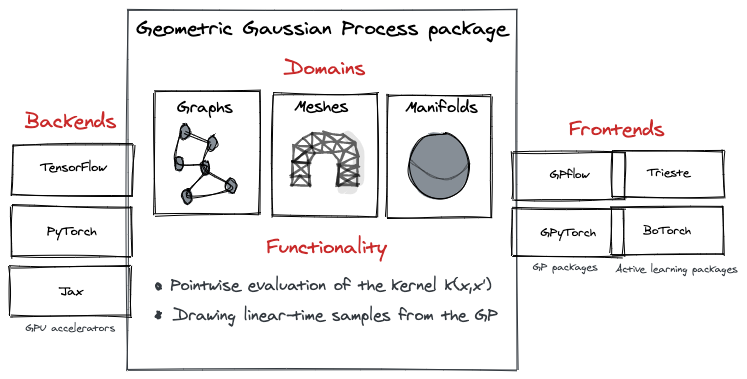
\includegraphics[width=.7\textwidth]{geomgp}
    \caption{Overview of Geometric Kernel package}
    \label{fig:geomgp}
\end{figure}

Open-source, high-quality software is a key katalysator for good research: it allows one to quickly prototype ideas on top of strong foundations, but---more importantly---it makes it possible to package mature research work to make it available to the wider community. The first objective is to develop a Python package which provides implementations of geometric kernels on analytic manifolds and. The package will also be opinionated on the best way to handle these objects for downstream tasks. However, to not hinder adoption by the wider community the package will be backend agnostic, which will allow for downstream use TensorFlow package (e.g., GPflow) and PyTorch packages (e.g., GPytorch). \Cref{fig:geomgp} gives an overview of the package. Development has started at \url{https://github.com/GPflow/GeometricKernels}.

\subsection{Efficiency: Sparse Manifold Gaussian processes}

The cubic computational complexity of GPs in Euclidian spaces limits their use in many real-world applications. As explained in \cref{chapter:theoretical-framework}, a widely adopted solution to this problem is to employ a smaller set of inducing points which summarise the GP at a set of optimised input locations. Not surprisingly, the same cubic computational complexity is present in the non-Euclidian counterpart of GPs. It is, unfortunately, not straightforward to extend the inducing point solution to these domains. For example, it is not clear how to define an inducing variable on a graph or on a mesh, and how one would freely optimise their location to minimse the KL divegence between true and approximate posterior---as is the case with traditional inducing point inputs. The interdomain and eigenfeatures inducing variable approach, introduced in \cref{chapter:theoretical-framework,chapter:vish}, seems a promising route as the resulting basisfunctions are fixed, and by construction optimally placed for a given geometry. The objective of this research project is to develop a scalable method for GPs on manifolds, akin to the methods that one has at their disposable in the Euclidian case. 

\subsection{Application: Sequential decision-making on non-Euclidian spaces}

To convince a wider audience to use these methods, it is important to show their practical usefulness on a real-world use-case.


Take into account the case of moving the search operation. Calculate expecations of costs associated to search missions. % This use-case could be a stepping-stone into more scientific applications such as , which are similar in vein to 

To illustrate this it woul
Bayesian search: airplane crash -> gravitational waves
ba


% Basically settings where DNNs are never going to be competitive with GPs - low-dim, very data-efficient, high-cost - not even if someone figures out how to do DNN uncertainty right, due to GP regret guarantees (under reasonable assumptions) matching the best possible regret achievable by any model/decision system.

% \paragraph{Related areas}
% \begin{enumerate}
%     \item Probabilistic numerics [Tubingen Manifesto, Osborne and Henning]. They are less interested in closing the loop and making decisions atop of the models. They usually plot the error bars on the estimator as their final result.
%     \item Bayesian optimisation methods. Special case.
% \end{enumerate}



%%% OLD:

% Through this line of work, I believe that we have showed that (deep) Gaussian processes are an interesting non-parametric alternative to Bayesian neural networks (BNNs). Our work differs from the conventional BNN literature in that we attempt to scale well-understood fully-Bayesian models (i.e. GPs) to big data settings, rather than the converse: starting from complex parametric models and trying to approximate Bayesian inference in them. The former strategy allows to gradually build up complexity into the models while maintaining their favourable properties, such as a marginal likelihood objective and good uncertainty quantifications.

% In what comes next, I want to separate the different regimes in which neural networks and Gaussian processes operate and thrive. For example, NNs can handle---and in practice require---very large datasets, whereas Gaussian process models are more comfortable in the small data regime. Neural networks, in the presence of large datasets, are extremely good at learning complex latent representations, as evidenced by the latest models in natural language processing and computer vision. Non-parametric Gaussian processes, on the contrary, work best on limited and noisy datasets. Datasets where each datapoint can be very expensive in terms of cost or time to obtain. I believe that this is a setting---in the era of deep learning---that has been under studied and valued, yet of high importance for many scientific or commercial applications.

% Many real-world problems can be described as inferring properties of an expensive black-box function $f: \mathcal{X} \rightarrow \mathcal{Y}$, subject to a computational budget of $T$ function evaluations. Typical examples are (global) optimisation, finding a level set (i.e. the set of points in $X \subset \mathcal{X}$ for which $f(x) > C,\forall x \in X$), or finding the shortest path between two nodes in a graph. In the graph example, the black-box function $f$ would return the cost of traversing an edge and query the cost of an edge would be very expensive. Naively applying Dijkstra would require the evaluation of $f$ at every edge and thus potentially grossly exceeding the given budget of $T$ evaluations.


% \begin{enumerate}
%     \item Black Box Functions $f: \mathcal{X} \rightarrow \mathcal{Y}$
%     \item We want to estimate a computable property $\mathcal{O}_\mathcal{A}(f)$
%     \item $\mathcal{A}$ is an algorithm $\mathcal{O}_\mathcal{A}(f) = \mathcal{A}(f)$
%     \item Evaluating $f$ is \emph{very} expensive (we can only evaluate it a limited amount of times)
% \end{enumerate}

% \paragraph{Examples}
% \begin{enumerate}
%     \item Optimisation: $\mathcal{A}(f) = \argmax_{x\in\mathcal{X}} f(x)$, which implies $\mathcal{O}_\mathcal{A}(f) = x^*$.
%     \item Sensor Placement (Active Learning): $\mathcal{O}_\mathcal{A}(f) = \argmax_{X \subset \mathcal{X}, |X| = T} \textrm{MI}(f, f(X))$.
%     \item Level sets: $\mathcal{O}_\mathcal{A}(f) = \{X \subset \mathcal{X}: f(x) > C, \forall x \in X\}$.
%     \item Shortest path: $\mathcal{O}_\mathcal{A}(f) = $ shortest path between two nodes in a graph.
% \end{enumerate}

% \paragraph{Real-world problems}
% \begin{itemize}
%     \item[Graphs] Social networks. Search for cliques or shortest paths.
%     \item[Meshes] Aerospace and civil engineering problems. ``General'' sensor placement.
%     \item[Manifold] Sphere. Interesting problem in astrophysics: when a gravitational wave detection is made there's usually a very large uncertainty of its origin so optical telescopes have to sweep the sky looking for the source.
% \end{itemize}

% \paragraph{Objectives}
% \begin{enumerate}
%     \item Theory and analysis
%     \item Show the excellence of Gaussian processes in this regime
%     \item Benchmarks for future methods
% \end{enumerate}
%\graphicspath{{Chapter5/Figs/}}

\chapter{Future Research Agenda}
\label{chapter:future-research}

\section{Introduction}
To date, my research has focussed on using Gaussian processes (GPs) as building blocks for deep models, similar to neural network layers. In this vein, I have worked on (1) deep convolutional Gaussian processes that mimic the convolutional and layered architectures encountered in many contempory deep learning models \citep{Dutordoir2020convolutional}, (2) conditional density estimation models which are similar to Variational Auto Encoders \citep{dutordoir2018cde,Salimbeni2019}, and (3) more recently, deep Gaussian processes that have basis functions that are similar to neural network activation functions \citep{dutordoir2021deep} (discussed at length in \cref{chapter:dnn-as-point-estimate-for-dgps}). I have packaged these advances in a software toolbox, called GPflux \citep{dutordoir2021gpflux}, which provides these GP layers through a neural network like interface. The main advantage of this approach is that straightforward application of Bayesian principles leads to sensible results, which is not necissarily the case for normal neural networks \citep{wenzel2020good}. The current state of research into using Gaussian processes as layers is that classification performance starting to be on-par with deep learning on simple datasets \citep{dutordoir2018cde}, but with good uncertainty quantification and automatic selection of hyperparameters working `out of the box'.

The primary focus of my previous research can be considered as `curve-fitting', i.e. finding the best function approximator when given examples of inputs and corresonponding outputs. In this setting we can consider two regimes: (1) the function is very complex but there is an abundance of high-quality and cheap data to learn the mapping, and (2) the function is of a simpler nature but the underlying data is limited, noisy and/or very expensive to acquire. As evidenced by many recent advances in domains such as natural language and vision, where indeed there is a large availablility of high-quality data, the first regime is a setting where deep learning thrives. The natural inductive bias of deep neural networks (DNNs) in combination with the low computational cost of training them on massive datasets has proven to be very effective. Arguably, performing (approximate) Bayesian inference in this regime will contribute little to the end result, and the computational cost associated with it makes it very cumbersome. 

The second regime, in which data is noisy, requires a completely different modelling paradigm. On the one hand, the noisy data forces the model to be uncertain about the signal that can be extracted from the given examples. On the other hand, the simpler nature of the function allows an expert to encode prior information about the problem at hand. This enables faster generalisation from little data, which can be necessary given the high cost of acquiring more. This is a setting where probabilistic Bayesian models thrive.

However, to fully valorise Bayesian models one needs to consider them as part of a larger `decision-making' system. In these systems probabilistic models can be used to determine optimal actions to take in order to achieve a certain outcome. % For example, finding the input value that minimises an unknown `black-box' function. % Since good decisions depend on the confidence of our knowledge, faithfully representing uncertainty is a crucial aspect of the models.

In the next chapter of my PhD, I want to evolve from purely `curve-fitting' applications to focusing more on decision-making systems that \emph{use} probabilistic models to drive their decisions. In particular, I want to focus on probabilistic models that take into account the geometry of the problem at hand. This will allow encorporating more accurately physical properties and constraints of the system under study. In the next section we briefly discuss Markov Decision Processes (MDPs), a formal mathematical framework to decision making. We pay attention to the model based approach. InSection we can define probabilistic models in non-Euclidian spaces. on  . We finish with suggesting concrete research topics and a real-world application.

% . I would like to focus on both the modelling side and the decision-making aspect using the model's outputs. In the next two sections we discuss the type of decision system we consider and how we can define Gaussian processes on these spaces. 

\section{Markov Decision Process}

A discrete-time Markov decision Process (MDP) is a stochastic control process. It provides a mathematical framework for decision making in situations where outcomes are partly random and partly under the control of a decision maker [CITE TODO]. A MDP is characterised by a 4-tuple, consiting of
\begin{enumerate}
    \item A state space $\mathcal{S}$,
    \item An action space $\mathcal{A}$,
    \item Reward density $p(r \given a, s)$: the immediate reward obtained after executing an action $a$ in a given state $s$,
    \item Transition density $p(s' \given a, s)$: transitioning from state $s$ to state $s'$, due to action $a$.
\end{enumerate}
It should be noted that this is a very broad definition, yet there are still many variations to it. For instance, one can consider deterministic reward and transition functions, continuous-time and partially observed MDPs.

The objective of an MDP is to find a `good' (probabilistic) policy function $\pi:\mathcal{S} \rightarrow \mathcal{X}$. This is a mapping that specifies which action a decision maker should take in a given state $s$. The goal is to find a sequence of actions, starting from an initial state $s_0$, that maximses the cumulative reward a decision maker obtains by obeying the policy $\pi$. This is given by the value function
\begin{equation}
    V^{(\pi)}(s_0) = \Exp{}{\sum_t r_t}
\end{equation}
where the expectation is over $r_t \sim p(r_t \given s_t, a_t)$, $s_{t+1} \sim p(s_{t+1} \given s_t, a_t)$ and $a_t \sim \pi(s_t)$.

The quality of a policy $\pi$ is given by the \emph{regret}, which measures the value function $V^{(\pi)}$ relative to the optimal value function $V^{*}$ obtained by the best possible policy $\pi^*$
\begin{equation}
    R^{(\pi)}(s_0) = V^*(s_0) - V^{(\pi)}(s_0). 
\end{equation}

\subsection{A Model-based Approach}
There are many different ways to deduct a good---or even an optimal---policy for a given MDP, but the exact algorithm will heavily depend on the precise formulation of the problem. Here, we consider the case that the transition and reward function are unknown, and also very expensive to evaluate. In this setting, any efficient algorithm will need to consider whether to take explorative actions that might lead to better rewards, or take advantage of actions that are known to be good but will not improve the current solution. This dilema is known as the exploitation-exploration trade-off. The fact that the functions are expensive to evaluate makes it worthwile to spend resources (e.g., time and compute) on deciding where to evaluate them next.

A strategy to address this MDP formulation is using a \emph{model-based} approach. Broadly speaking, this approach consists of a model that learns the unknown transitions and/or rewards from observed data in a supervised learning way. Subsequently, a policy is derived using the learned model rather than using the true reward and transition functions. % The exploitation-exploration trade-off highlights the importance of the model to faitfully represent the uncertainty present in the data.

\paragraph{Example}
We consider Bayesian optimisation (BO) [CITE] as an illustration of these concepts. BO is a sequential search algorithm for finding a global minimiser of an unknown objective function $f$ defined over a domain of interest $\mathcal{X}$
\begin{equation}
    x_* = \argmin_{x \in \mathcal{X}} f(x).
\end{equation}
The function $f$ is not observed directly. Instead, at each step the algorithm selects a query point $x \in \mathcal{X}$ at which to evaluate $f$ and obtains $y(x)$: a function evaluation corrupted by noise $y(x) \sim p(y(x) \given f(x))$. 

BO can be framed as a MDP if one considers the cardinality of $\mathcal{S}$ to be $1$, and the actions space to cover the function's input domain $\mathcal{A} = \mathcal{X}$. As there is only a single state the transition functions trivially reduces to the identity function. The reward associated to an action $x$\footnote{To adhere to the common notation in BO we use $x$, rather than $a$, to represent the action (in our case the next query point).} is given by the negative function observation. This construction leads to an unknown and probabilistic reward  function due to the unknown objective function and the noisy observations. Collecting the sequence of actions (i.e. query points) $\{x_t\}$, the performance of an algoritm selecting the query points can be measured using a tailered notion of reget
\begin{equation}
    R = \sum_t f(x_t) - f(x_*).
\end{equation}

A model-based approach to this problem employs a surrogate model $g$ which learns the unknown objective function $f$ using past observations. The surrogate model is used to decide on the next query point, through what is known as an \emph{acquisition rule} [CITE]. The exploitation-exploration trade-off highlights the importance of the surrogate model's faithful represention of uncerainty about the objective. It is a key ingredient to an effective algorithm and is necessary to obtain a low regret [CITE]. Most model-based approaches employ Gaussian processes (GPs) as their surrogate model: $g \sim \GP$ [CITE]. 

To follow a model-based approach in Bayesian optimisation, as well as in other kinds of MDPs, it is required to define a GP on the domain of interest. For convenience, this domain is typically chosen to be the Euclidian space. However, many problems possess important non–Euclidean geometric structure, which makes it much more effective and convenient to directly specify the problem on the non-Euclidean domain, like the torus or the sphere, but also a graph, a rotation group, or the space of positive-definite matrices. Consider for example optimising the joint postures of a robot, which are defined on the torus $\mathcal{T}^d = \mathcal{S}^1 \times \mathcal{S}^1 \ldots \times \mathcal{S}^1$. To accomodate for this, one must be able to specify a GP prior, or equivalently define a kernel, on this space of interest.

\section{Gaussian Processes as Surrogate Models in non-Euclidian manifolds}

\begin{figure}[tbh!]
  \centering
\begin{subfigure}{0.3\textwidth}
  \vspace{.3cm}
  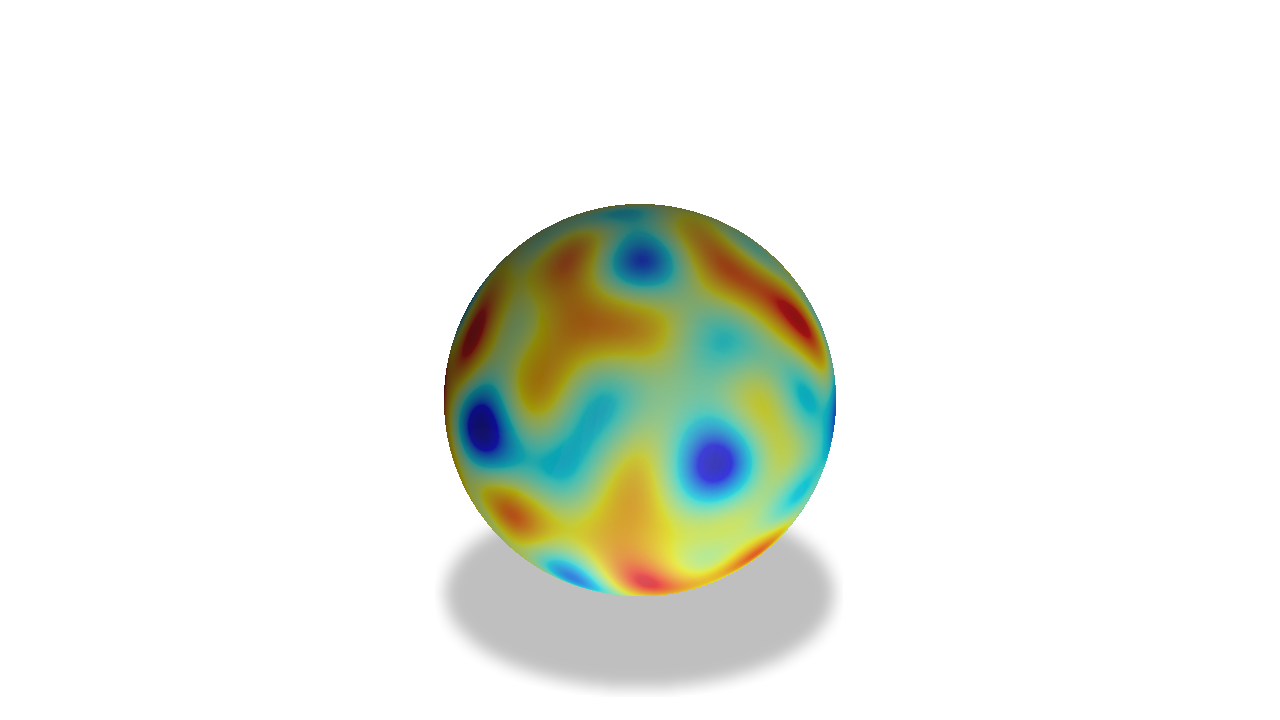
\includegraphics[clip, trim=12cm 0cm 12cm 7cm,width=\textwidth]{sphere}
  \caption{Sphere}
  \label{fig:sphere}
\end{subfigure}\hfil % <-- added
\begin{subfigure}{0.3\textwidth}
  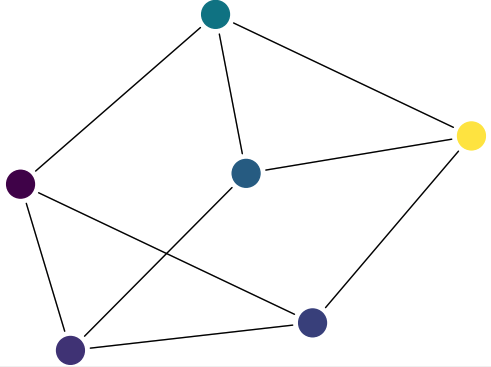
\includegraphics[clip, trim=0cm .05cm 0cm 0cm, width=\textwidth]{graph}
  \vspace{.5cm}
  \caption{Graph}
  \label{fig:graph}
\end{subfigure}\hfil % <-- added
\begin{subfigure}{0.3\textwidth}
  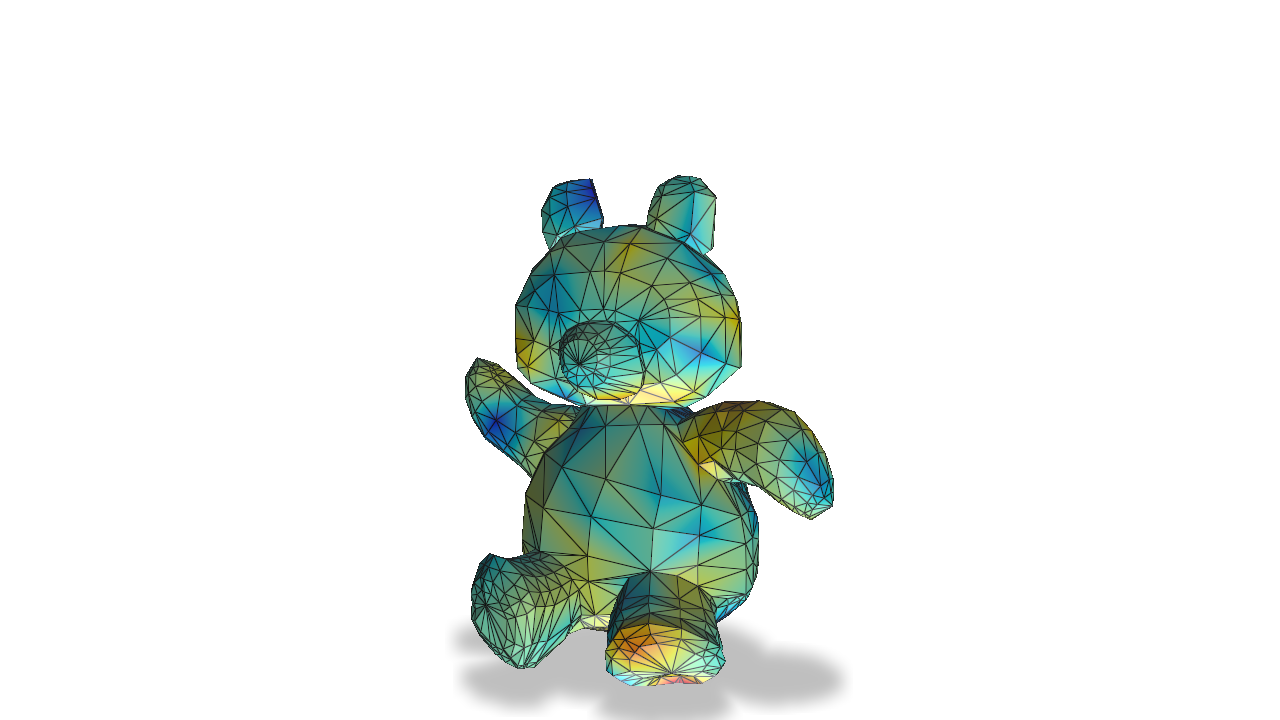
\includegraphics[clip, trim=12cm 0cm 12cm 5cm,width=\textwidth]{teddy_mesh}
  \caption{Mesh}
  \label{fig:mesh}
\end{subfigure}
\caption{Mat\'ern GP samples on non-Euclidian spaces}
\label{fig:xxxx}
\end{figure}

Stationary kernels are ubiquitous in Gaussian processes when the input space is Euclidean. Their popularity is due to their general useability and the ease of understanding which prior information they encode. Recent work of \citet{Borovitskiy2020} has extended the definition of stationary kernels to Riemannian manifolds. This enables the definition of symmetric and positive-definite kernels, which characterise GPs, that take into account the geometry of the space. In the case of a graph, for example, two nodes can be close to each other in the Euclidean space yet far apart in the term of number of edges them separates them. A classical statioary kernel is not able to capture this information, whereas a geometric aware kernel can.

The construction in \citet{Borovitskiy2020} relies on the spectral theory of the Laplace-Beltrami operator and defines the kernel through its Mercer decomposition (\cref{eq:mercer})
\begin{equation}
    \label{eq:borovitskiy}
    k(x, x) = \sum_i S(\sqrt{\lambda_i})\,\phi_i(x)\,\phi_i(x')
\end{equation}
where $S$ is the power spectrum of the kernel and $\{\lambda_i, \phi_i\}$ are the eigenvalues and eigenfunctions of the Laplace-Beltrami operator. \cref{chapter:vish} discusses a special case of this construction for zonal kernels defined on the hypersphere where the eigenfunctions are given by the spherical harmonics.

The elegance of \cref{eq:borovitskiy} is that it defines the kernel through the eigenfunctions of the Laplace-Beltrami operator. These eigenfunctions are known analytically for certain well-studied manifolds, such as the sphere and the torus. However, in practice, working with more complex manifolds involves descretizing the manifold of which the mesh and undirected weighted graph are special cases. This simple framework allows us to unify these spaces and allows us to develop apply to all of them.

Given the brief background on model-based approaches to MDP and Gaussian processes defined on non-Euclidian spaces we now suggest the following projects 

\section{Research Agenda}
The overarching theme of my proposed research agenda is: ``How can we make Gaussian processes an effective tool for decision-making tasks on non-Euclidean spaces?''. The goal would be that these tools are more widely used outside our `small' GP community by scientist and engineers who deal with these problems regularily. One could envision these tools to be particularly useful in domains such as mechanical engineering where finite element meshes, environmental modelling which is often done on the sphere, and bio-medical applications on organ-shaped manifolds. To achieve this goal we need at least the following components:

\subsection{Adopotion: Geometric Kernel Package}

\begin{figure}
    \centering
    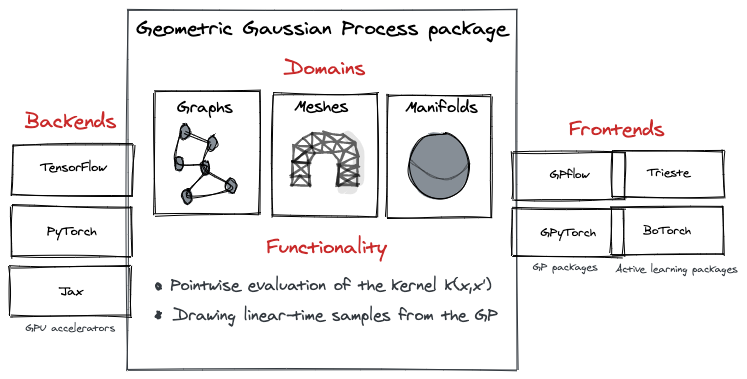
\includegraphics[width=.7\textwidth]{geomgp}
    \caption{Overview of Geometric Kernel package}
    \label{fig:geomgp}
\end{figure}

Open-source, high-quality software is a key katalysator for good research: it allows one to quickly prototype ideas on top of strong foundations, but---more importantly---it makes it possible to package mature research work to make it available to the wider community. The first objective is to develop a Python package which provides implementations of geometric kernels on analytic manifolds and. The package will also be opinionated on the best way to handle these objects for downstream tasks. However, to not hinder adoption by the wider community the package will be backend agnostic, which will allow for downstream use TensorFlow package (e.g., GPflow) and PyTorch packages (e.g., GPytorch). \Cref{fig:geomgp} gives an overview of the package. Development has started at \url{https://github.com/GPflow/GeometricKernels}.

\subsection{Efficiency: Sparse Manifold Gaussian processes}

The cubic computational complexity of GPs in Euclidian spaces limits their use in many real-world applications. As explained in \cref{chapter:theoretical-framework}, a widely adopted solution to this problem is to employ a smaller set of inducing points which summarise the GP at a set of optimised input locations. Not surprisingly, the same cubic computational complexity is present in the non-Euclidian counterpart of GPs. It is, unfortunately, not straightforward to extend the inducing point solution to these domains. For example, it is not clear how to define an inducing variable on a graph or on a mesh, and how one would freely optimise their location to minimse the KL divegence between true and approximate posterior---as is the case with traditional inducing point inputs. The interdomain and eigenfeatures inducing variable approach, introduced in \cref{chapter:theoretical-framework,chapter:vish}, seems a promising route as the resulting basisfunctions are fixed, and by construction optimally placed for a given geometry. The objective of this research project is to develop a scalable method for GPs on manifolds, akin to the methods that one has at their disposable in the Euclidian case. 

\subsection{Application: Sequential decision-making on non-Euclidian spaces}

To convince a wider audience to use these methods, it is important to show their practical usefulness on a real-world use-case.


Take into account the case of moving the search operation. Calculate expecations of costs associated to search missions. % This use-case could be a stepping-stone into more scientific applications such as , which are similar in vein to 

To illustrate this it woul
Bayesian search: airplane crash -> gravitational waves
ba


% Basically settings where DNNs are never going to be competitive with GPs - low-dim, very data-efficient, high-cost - not even if someone figures out how to do DNN uncertainty right, due to GP regret guarantees (under reasonable assumptions) matching the best possible regret achievable by any model/decision system.

% \paragraph{Related areas}
% \begin{enumerate}
%     \item Probabilistic numerics [Tubingen Manifesto, Osborne and Henning]. They are less interested in closing the loop and making decisions atop of the models. They usually plot the error bars on the estimator as their final result.
%     \item Bayesian optimisation methods. Special case.
% \end{enumerate}



%%% OLD:

% Through this line of work, I believe that we have showed that (deep) Gaussian processes are an interesting non-parametric alternative to Bayesian neural networks (BNNs). Our work differs from the conventional BNN literature in that we attempt to scale well-understood fully-Bayesian models (i.e. GPs) to big data settings, rather than the converse: starting from complex parametric models and trying to approximate Bayesian inference in them. The former strategy allows to gradually build up complexity into the models while maintaining their favourable properties, such as a marginal likelihood objective and good uncertainty quantifications.

% In what comes next, I want to separate the different regimes in which neural networks and Gaussian processes operate and thrive. For example, NNs can handle---and in practice require---very large datasets, whereas Gaussian process models are more comfortable in the small data regime. Neural networks, in the presence of large datasets, are extremely good at learning complex latent representations, as evidenced by the latest models in natural language processing and computer vision. Non-parametric Gaussian processes, on the contrary, work best on limited and noisy datasets. Datasets where each datapoint can be very expensive in terms of cost or time to obtain. I believe that this is a setting---in the era of deep learning---that has been under studied and valued, yet of high importance for many scientific or commercial applications.

% Many real-world problems can be described as inferring properties of an expensive black-box function $f: \mathcal{X} \rightarrow \mathcal{Y}$, subject to a computational budget of $T$ function evaluations. Typical examples are (global) optimisation, finding a level set (i.e. the set of points in $X \subset \mathcal{X}$ for which $f(x) > C,\forall x \in X$), or finding the shortest path between two nodes in a graph. In the graph example, the black-box function $f$ would return the cost of traversing an edge and query the cost of an edge would be very expensive. Naively applying Dijkstra would require the evaluation of $f$ at every edge and thus potentially grossly exceeding the given budget of $T$ evaluations.


% \begin{enumerate}
%     \item Black Box Functions $f: \mathcal{X} \rightarrow \mathcal{Y}$
%     \item We want to estimate a computable property $\mathcal{O}_\mathcal{A}(f)$
%     \item $\mathcal{A}$ is an algorithm $\mathcal{O}_\mathcal{A}(f) = \mathcal{A}(f)$
%     \item Evaluating $f$ is \emph{very} expensive (we can only evaluate it a limited amount of times)
% \end{enumerate}

% \paragraph{Examples}
% \begin{enumerate}
%     \item Optimisation: $\mathcal{A}(f) = \argmax_{x\in\mathcal{X}} f(x)$, which implies $\mathcal{O}_\mathcal{A}(f) = x^*$.
%     \item Sensor Placement (Active Learning): $\mathcal{O}_\mathcal{A}(f) = \argmax_{X \subset \mathcal{X}, |X| = T} \textrm{MI}(f, f(X))$.
%     \item Level sets: $\mathcal{O}_\mathcal{A}(f) = \{X \subset \mathcal{X}: f(x) > C, \forall x \in X\}$.
%     \item Shortest path: $\mathcal{O}_\mathcal{A}(f) = $ shortest path between two nodes in a graph.
% \end{enumerate}

% \paragraph{Real-world problems}
% \begin{itemize}
%     \item[Graphs] Social networks. Search for cliques or shortest paths.
%     \item[Meshes] Aerospace and civil engineering problems. ``General'' sensor placement.
%     \item[Manifold] Sphere. Interesting problem in astrophysics: when a gravitational wave detection is made there's usually a very large uncertainty of its origin so optical telescopes have to sweep the sky looking for the source.
% \end{itemize}

% \paragraph{Objectives}
% \begin{enumerate}
%     \item Theory and analysis
%     \item Show the excellence of Gaussian processes in this regime
%     \item Benchmarks for future methods
% \end{enumerate}
%\include{Chapter6/chapter6}
%\include{Chapter7/chapter7}



% ********************************** Back Matter *******************************
% Backmatter should be commented out, if you are using appendices after References
%\backmatter

% ********************************** Bibliography ******************************
\begin{spacing}{0.9}

% To use the conventional natbib style referencing
% Bibliography style previews: http://nodonn.tipido.net/bibstyle.php
% Reference styles: http://sites.stat.psu.edu/~surajit/present/bib.htm

% \bibliographystyle{apalike}
%\bibliographystyle{unsrt} % Use for unsorted references  
%\bibliographystyle{plainnat} % use this to have URLs listed in References
\cleardoublepage
\printbibliography[title=References]

% \bibliography{References/references} % Path to your References.bib file


% If you would like to use BibLaTeX for your references, pass `custombib' as
% an option in the document class. The location of 'reference.bib' should be
% specified in the preamble.tex file in the custombib section.
% Comment out the lines related to natbib above and uncomment the following line.

%\printbibliography[heading=bibintoc, title={References}]


\end{spacing}

% ********************************** Appendices ********************************

\begin{appendices} % Using appendices environment for more functunality
\crefalias{section}{appendix}
\crefalias{chapter}{appendix}

%!TEX root = ../thesis.tex
% ******************************* Thesis Appendix A ****************************
\chapter{Spherical Harmonics on Hyperspheres} 
\label{appendix:spherical-harmonics}

Spherical harmonics are a special set of functions defined on the hypersphere and play a central role in harmonic analysis and approximation theory \citep{wendland2005}. They originate from solving Laplace's equation, and form a complete set of orthogonal functions. Any sufficiently regular function defined on the sphere can be written as a sum of these spherical harmonics, similar to the Fourier series with sines and cosines. Spherical harmonics are defined in arbitrary dimensions \citep{frye2014,dai2013}, but lack explicit formulations and practical implementations in dimensions larger than three. %This is mainly due to the complexity of solving Laplace's equation in higher dimensions.

In this section, we propose a novel algorithm to construct spherical harmonics in $d$ dimensions. The algorithm is based on the existence of a fundamental system of points on the hypersphere, which we select in a greedy fashion through optimisation. This result in spherical harmonics that are a linear combination of zonal functions and form an ortho-normal basis on $\dsphere$. The algorithm lends itself well for implementation in Python and TensorFlow, which we provide at: \url{https://github.com/vdutor/SphericalHarmonics}. The code is accompanied by a series of tests that show that the properties of spherical harmonics, as detailed below, hold. Before outlining the algorithm, we briefly define and cover the important properties of spherical harmonics in $\Reals^d$. We refer the interested reader to \citet{dai2013,frye2014} for a comprehensive overview.
% exist bases of spherical harmonics consisting of entirely zonal harmonics

We adopt the usual $L_2$ inner product for functions $f: \dsphere \rightarrow \Reals$ and $g: \dsphere \rightarrow \Reals$ restricted to the sphere 
\begin{equation}
     \langle f, g\rangle_{L_{2}(\dsphere)} = \frac{1}{\darea} \int_{\dsphere} f(x)\,g(x) \, \calcd{\omega},
\end{equation}
where $\calcd{\omega(x)}$ is the surface area measure such that $\darea$ denotes the surface area of $\dsphere$ 
\begin{equation}
\label{eq:surface}
    \darea = \int_{\dsphere} \calcd{\omega(x)} = \frac{2 \pi ^ {d/2}}{\Gamma(d/2)}.
\end{equation}

Throughout this section we use the following notation and definitions. For $x = (x_1, \ldots, x_d) \in \Reals^d$ and $\alpha = (\alpha_1, \ldots, \alpha_d) \in \Naturals^d$, a monomial $x^\alpha$ is a product $x^\alpha = x_1^{\alpha_1} \ldots x_d^{\alpha_d}$, which has degree $|\alpha| = \alpha_1 + \ldots \alpha_d$. A real homogeneous polynomial $P(x)$ of degree $n$ is a linear combination of monomials of degree $n$ with real coefficients, that is $P(x) = \sum_{|\alpha| = n} c_{\alpha} x^{\alpha}$, with $c_\alpha \in \Reals$. We denote $\mathcal{P}_n^d$ as the space of real homogeneous polynomials of degree $n$, and can show that, counting the cardinality of the set $\{\alpha \in \Naturals^d: |\alpha| = n\}$, that $\dim(\mathcal{P}_n^d) = \binom{n + d -1}{n}$. A function $f:\Reals^d \rightarrow \Reals$ is said to be \emph{harmonic} if $\Delta f = 0$, where $\Delta = \partial_{x_1}^2 + \ldots + \partial_{x_d}^2$ and $\partial_{x_i}$ the partial derivate w.r.t. the $i$-th variable.

\begin{definition}
    The spherical harmonics of degree $n$ of $d$ variables, denoted by $\mathcal{H}_{n}^d$, is the linear space of harmonic and homogeneous in degree $n$ polynomials on $\dsphere$, that is 
    \begin{equation}
        \mathcal{H}_{n}^d = \{p \in \mathcal{P}_n^d: \Delta p = 0\ \text{and}\ p: \dsphere \rightarrow \Reals \}.
    \end{equation}
The dimensionality of $ \mathcal{H}_{n}^d$ is given by
\begin{equation}
\label{eq:numharmonics}
\dim(\mathcal{H}_{n}^d) = \frac{2 n + d - 2}{n} \binom{n + d - 3}{d - 1} := \dnumharmonicsforlevel.
\end{equation}
\end{definition}

The space $\mathcal{H}_{n}^d$ has an orthonormal basis consisting of $\dnumharmonicsforlevel$ functions, denoted by $\{\phi_{n,j}\}_{j=1}^{\dnumharmonicsforlevel}$. The basis satisfy the following properties
\begin{equation}
    \mathcal{H}_{n}^d  = \textrm{span}\left(\phi_{n,1}, \ldots, \phi_{n, \dnumharmonicsforlevel}\right),\quad\text{and}\quad\left\langle \phi_{n, j}, \phi_{n', j'}\right\rangle_{L_2(\dsphere)} = \delta_{n n'} \delta_{j j'}.
\end{equation}

From the completeness and orthonormality of the spherical harmonic basis $\{\phi_{n,j}\}_{n=0,j=1}^{\infty,\dnumharmonicsforlevel}$, it can be shown that they also form a basis of square-integrable functions \citep{frye2014}. This means that we can decompose a function $f: \dsphere \rightarrow \Reals$ as
\begin{equation}
    f = \sum_{n=0}^{\infty} \sum_{j=1}^{\dnumharmonicsforlevel} \widehat{f}_{n, j} \phi_{n, j},\quad\text{with}\quad\widehat{f}_{n, j} = \langle f, \phi_{n, j} \rangle_{L_2(\dsphere)},
\end{equation}
which can be seen as the spherical analogue of the Fourier decomposition of periodic functions onto a basis of sines and cosines.

Subsequently, we will coin the set $\{\phi_{n,j}\}$ as the spherical harmonics. They are indexed by $n$ and $j$, where $n=0,1,2,\ldots$ denotes the degree (or level) and $j=1,\cdots,\dnumharmonicsforlevel$ denotes the orientation of the spherical harmonic. We are interested in finding $\{\phi_{n,j}\}$ in arbitrary dimension. For $d=2$, is solving Laplace's equation ($\Delta p = 0$) directly relatively straightforward. Doing so reveals that $N^{2}_0 = 1$ with $\phi_{0, 1} = 1$ and $N^{2}_n = 2$ for all $n > 0$ with $\phi_{n, 1}(\theta) = \sqrt{2} \cos(n \theta)$ and $\phi_{n, 2}(\theta) = \sqrt{2} \sin(n \theta)$. This shows that on the unit circle $\sphere^1$, the spherical harmonics correspond to the Fourier basis. For $d=3$, we can also directly solve Laplace's diffential equation to find $\dnumharmonicsforlevel = 2n + 1$ and a closed form solution for $\{\phi_{n,j}\}$. However, for $d > 3$, explicit formulations for the spherical harmonics become very rare. To the best of our knowledge, the only explicit formulation we could find is in \citet[Theorem~5.1]{dai2013}, which consists of a product over polynomials. This makes the implementation cumbersome and numerically unstable, and only practically useful up to 10 dimensions \citep{Dutordoir2020spherical}. However, making use of the following two theorems, we can derive another formulation for the basis of spherical harmonics as a sum of polynomials, rather than a product. The connection between spherical harmonics and orthogonal polynomials becomes clear in the next theorem.
\begin{theorem}[Addition]
    \label{theorem:addition}
    Let $\{\phi_{n,j}\}_{j=1}^{\dnumharmonicsforlevel}$ be an orthonormal basis for the spherical harmonics of degree $n$ and $x,x' \in \dsphere$. Then the Gegenbauer polynomial $C_n^{(\alpha)}: [-1, 1] \rightarrow \Reals$ of degree $n$ can be written as
\begin{equation}
    \sum_{j=1}^{\dnumharmonicsforlevel} \phi_{n, j}(x) \phi _{n, j}(x') = \frac{n + \alpha}{\alpha}\,
    C_n^{(\alpha)}(x\transpose x')\quad\text{with}\quad \alpha = \frac{d-2}{2}.
\end{equation}
\end{theorem}
As a result of the relation between the Gegenbauer polynomial and the spherical harmonics, are the Gegenbauer polynomial sometimes referred to as ultraspherical polynomials. For $d=2$, Theorem~1 recovers the addition formula of the cosine function, as indeed $\cos(\theta) \cos(\theta') + \sin(\theta) \sin(\theta') = \cos(\theta - \theta')$ and $C_n^{(0)}(t) = \cos(n \arccos(t))$. The Gegenbauer polynomials with $\alpha=0$ are better known as the Chebyshev polynomials. Another connection between spherical harmonics and Gegenbauer polynomials is given by the Funk-Hecke theorem and applies to zonal functions. A zonal function on $\dsphere$ is a function that is rotationally invariant w.r.t. to a point on the sphere, $\eta \in \dsphere$. This means that the function only depends on the inner product $\eta\transpose x$, or equivalently, on the geodestic distance between $\eta$ and $x$.

\begin{theorem}[Funk-Hecke]
    \label{appendix:theorem:funk}
    Let $f$ be an integrable function such that $\int_{-1}^1 \| f(t)\| (1 - t^2)^{(d-3)/2} \calcd{t}$ is finite and $d \ge 2$. Then for every $\phi_{n,j}$  and $\eta \in \dsphere$
    \begin{equation}
        \frac{1}{\darea} \int_{\dsphere} f(\eta\transpose x)\,\phi_{n, j}(x)\, \calcd{\omega(x)} = {\lambda}_{n}\,\phi_{n,j}(\eta),
    \end{equation}
    where ${\lambda}_{n}$ is a constant defined by
    \begin{equation}
        \lambda_{n}  = 
        % \frac{\Omega_{d-2}}{\Omega_{d-1}} 
        \frac{\omega_{d}}{C_n^{(\alpha)}(1)} \int_{-1}^1 f(t)\,C_n^{(\alpha)}(t)\,(1 - t^2)^{\frac{d-3}{2}} \calcd{t},
    \end{equation}
    with $\alpha = \frac{d-2}{2}$ and $\omega_d = \frac{\Omega_{d-2}}{\Omega_{d-1}}$.
\end{theorem}

\section{Algorithm: Zonal Spherical Harmonics}
\label{sec:zonal-spherical-harmonics}

From the Funk-Hecke and the Addition theorem, it is clear that there is a strong connection between spherical harmonics and Gegenbauer polynomials. The next theorem develops this connection further as it states that a basis for spherical harmonics can be written as zonal Gegenbauer polynomials. % , that is $\phi_{n,j}(x) = \sum_i \beta_{j,i} C_n^{(\alpha)}(\eta_i\transpose x)$. In what comes next we show how to select the weights $\beta_{j,i}$ and zonal directions $\eta_i \in \dsphere$.

\begin{theorem}
    If $\{\eta_1, \ldots, \eta_{\dnumharmonicsforlevel} \} \in \dsphere$ is a fundamental system of points on the sphere, then $\{C_n^{(\alpha)}(\eta_i \cdot)\}_{i=1}^{\dnumharmonicsforlevel}$ is a basis for $\mathcal{H}_n^d$. A collection of points $\{\eta_1, \ldots, \eta_M \} \in \dsphere$ is called a fundamental system of degree $n$ consisting of $M$ points on the sphere if
    \begin{equation}
        \label{eq:fundamental-system}
        \textrm{det}\ 
        \begin{bmatrix}
            C_n^{(\alpha)}(1) & \ldots & C_n^{(\alpha)}(\eta_1\transpose\eta_M) \\
            \vdots & & \vdots \\
            C_n^{(\alpha)}(\eta_M\transpose\eta_1) & \ldots & C_n^{(\alpha)}(1)
        \end{bmatrix} > 0.
    \end{equation}
\end{theorem}
Finding a basis for $\mathcal{H}_n^d$ is thus equivalent to finding a set of $\dnumharmonicsforlevel$ points that satisfy \cref{eq:fundamental-system}. Crucially, \citet[Lemma~3]{dai2013} show that there always exists a fundamental system of degree $n$ and $\dnumharmonicsforlevel$ points.

Following the theorem, if we wish to construct $\{\phi_{n,j}\}_{n,j}$, an \emph{ortho-normal} basis for the spherical harmonics, we firstly need a fundamental system of points. Secondly, while $\{C_n^{(\alpha)}(\eta_i \cdot)\}_{i=1}^{\dnumharmonicsforlevel}$ forms a basis for $\mathcal{H}_n^d$, the basis is not orthonormal. We will thus have to apply a Gram-Schmidt process for ortho-normalising the basis. We detail both steps in the next paragraphs.

\paragraph{Construction of a fundamental system of points}
We propose to build a fundamental system of points in a greedy fashion by repeatedly adding a point on the sphere that maximises the determinant as given in \cref{eq:fundamental-system}. Therefore, let $\veta = \{\eta_1, \ldots, \eta_M\}$ contain the M points that are already in the fundamental system and define the following block-matrix of size $(M+1) \times (M+1)$ as
\begin{equation}
    \renewcommand\arraystretch{1.3}
    \MM(\veta, \eta_{*}) =
    \left[
        \begin{array}{c|c}
          C_n^{\alpha}(\veta\veta\transpose) \in \Reals^{M \times M} & C_n^{(\alpha)}(\veta\eta_{*}\transpose) \in \Reals^{M \times 1} \\
          \hline
          C_n^{(\alpha)}(\veta\eta_{*}\transpose)\transpose \in \Reals^{1 \times M} & C_n^{(\alpha)}(1) \in \Reals
        \end{array}
    \right],
\end{equation}
where $C_n^{(\alpha)}(\veta\veta\transpose)$ corresponds to element wise evaluating the Gegenbauer polynomial $C_n^{(\alpha)}: [-1, 1] \rightarrow \Reals$ for each element of $\veta \veta\transpose \in \Reals^{M \times M}$. A new point $\eta$ is added to the fundamental system if it maximises the determinant
\begin{equation}
    \eta = \argmax_{\eta_* \in \dsphere}\ \textrm{det}\left(\MM(\veta, \eta_{*})\right),
\end{equation}
in order to satisfy the condition in \cref{eq:fundamental-system}.
% \begin{equation}
%     \textrm{det}(\MC_n^{(\alpha)}(\veta, \eta_{*})) = \textrm{det}(C_n^{(\alpha)}(\veta\veta\transpose))\left(C_n^{(\alpha)}(1) - C_n^{(\alpha)}(\eta_{*}\veta\transpose) \left[C_n^{(\alpha)}(\veta\veta\transpose)\right]^{-1} C_n^{(\alpha)}(\veta\eta_{*}\transpose) \right).
% \end{equation}
Computing the determinant can be done efficiently using Schur' complement. Furthermore, as $\veta$ and $C_n^{(\alpha)}(1.0)$ are constants the optimisation problem boils down to
\begin{equation}
    \label{eq:optimisation-determinant}
    \eta = \argmin_{\eta_* \in \Reals^d}\ C_n^{(\alpha)}(\frac{\eta_{*}}{\norm{\eta_*}}\veta\transpose) \left[C_n^{(\alpha)}(\veta\veta\transpose)\right]^{-1} C_n^{(\alpha)}(\veta\frac{\eta_{*}\transpose}{\norm{\eta_*}}).
\end{equation}
The complete algorithm is given in \cref{alg:fundamental-system}.

\begin{algorithm}[H]
    \SetAlgoLined
    \DontPrintSemicolon
    \KwInput{Degree $n$ and dimension $d$}
    \KwResult{Fundamental system $\veta = \{\eta_0, \ldots \eta_{\dnumharmonicsforlevel}\}$}
    $\eta_1 = (0,0,\ldots,1)$ \tcp*{d-dimensional vector pointing north}
    $\veta = \{\eta_1\}$,
    $\alpha = \frac{d-2}{2}$,
    $i = 2$\;
     \While{$i \le \dnumharmonicsforlevel$}{
        $\eta = \argmax_{\eta_* \in \Reals^d}\ \textrm{det}(\MM(\veta, \frac{\eta_{*}}{\norm{\eta_*}}))$
        \tcp*{Using a local optimisation method (e.g., BFGS) and \cref{eq:optimisation-determinant}}
        Add $\eta$ to $\veta$\;
        i = i + 1\;
      }
     \caption{Construction of fundamental system\label{alg:fundamental-system}}
\end{algorithm}

\paragraph{Ortho-normalisation}

\begin{theorem}
   Let $\veta = \{\eta_1, \ldots, \eta_{\dnumharmonicsforlevel}\}$ be a fundamental system of degree $n$ consisting of $\dnumharmonicsforlevel$ points, and $\ML$ the inverse Cholesky factor of $C_n^{(\alpha)}(\veta\veta\transpose)$. Then for $j=1,\ldots,\dnumharmonicsforlevel$ and
    \begin{equation}
    \phi_{n,j}(x) = \sum_{i=1}^{\dnumharmonicsforlevel} \ML_{j,i}\,C_n^{(\alpha)}(\eta_i\transpose x)
    \end{equation}
    is $\{\phi_{n,j}\}$ an ortho-normal basis for the spherical harmonics $\mathcal{H}_n^d$.
\end{theorem}

The proof follows from $\langle C_n^{(\alpha)}(\eta_i\transpose \cdot), C_n^{(\alpha)}(\eta_j\transpose \cdot) \rangle_{L_2(\dsphere)} = C_n^{(\alpha)}(\eta_i\transpose\eta_j)$ as a result of the Funk-Hecke theorem.


% Let $\MM = C_n^{(\alpha)}(\veta\veta\transpose)$ and $\ML \ML\transpose = \MM$, which exists because the set $\veta$ satisfies \cref{eq:fundamental-system}.
% \begin{equation}
% \phi_{n,j}(x) = \sum_i [\ML\inv]_{j,i} C_n^{(\alpha)}(\eta_i\transpose x)
% \end{equation}

\begin{figure}
    \centering
    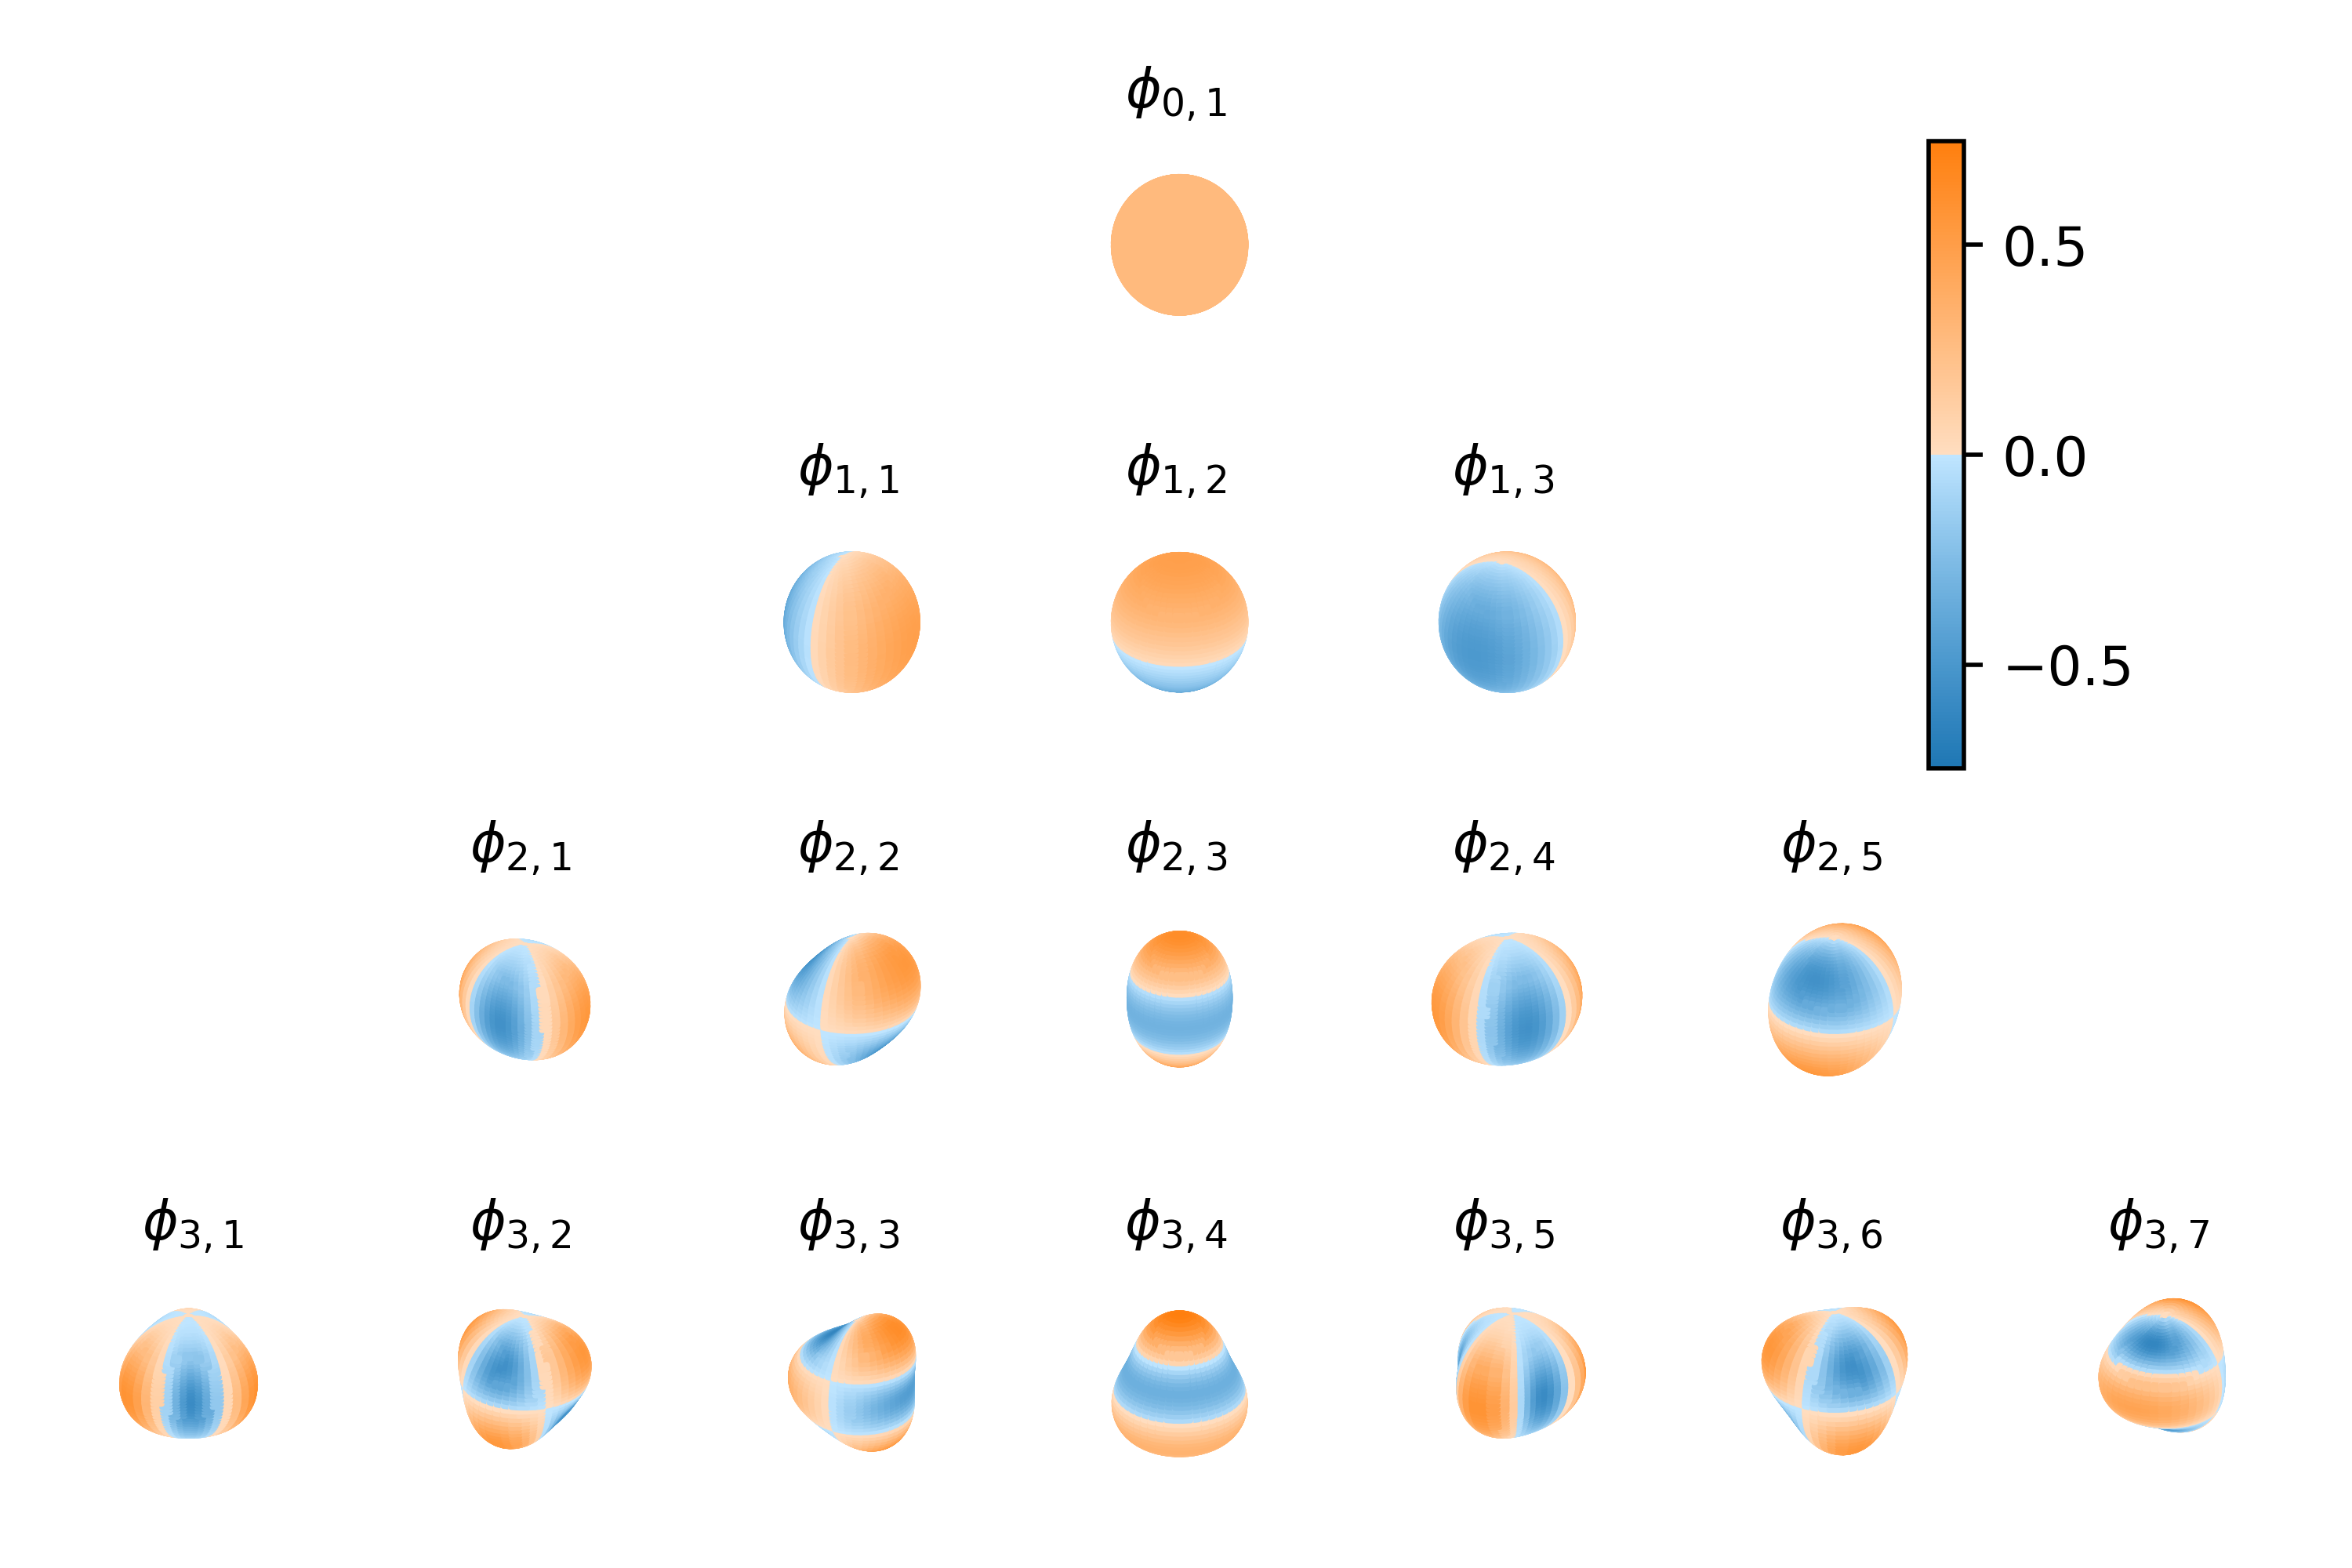
\includegraphics[width=.6\linewidth]{Appendix1/harmonics}
    \caption{Spherical Harmonics}
    \label{fig:appendix:harmonics}
\end{figure}
%!TEX root = ../thesis.tex
% ******************************* Thesis Appendix B ********************************

\chapter{Analytic computation of eigenvalues for zonal functions}
\label{app:sec:compute-eigenvalues}


The eigenvalues of a zonal function are given by the one-dimensional integral:
\begin{equation}
    \label{appendix:theorem:funk2}
    \lambda_{n} = 
   \frac{\omega_{d}}{C_n^{(\alpha)}(1)} \int_{-1}^1 s(t)\,C_n^{(\alpha)}(t)\,(1 - t^2)^{\frac{d-3}{2}} \calcd{t},
\end{equation}
where $C_n^{(\alpha)}(\cdot)$ is the Gegenbauer polynomial of degree $n$ with $\alpha = \frac{d-2}{2}$ and $\omega_{d} = \Omega_{d-2} / \Omega_{d-1}$ denotes the surface area of $\dsphere$ (see \cref{app:sec:harmonics} for analytical expressions of these quantities). The shape function $s(t)$ determines whether this integral can be computed in closed-form. In the next sections we derive analytical expressions for the eigenvalues of the Arc Cosine kernel and ReLU activation function in the case the $d$ is odd. For $d$ even, other kernels (e.g., Mat\'ern) or activation functions (e.g., Softplus, Swish, etc.) we rely on numerical integration (e.g., Gaussian quadrature) to obtain these coefficients. We will show that both approaches lead to highly similar results.

\section{Arc Cosine kernel}
\label{sec:appendix:compute-eigenvalues-arccosine}

The shape function of the first-order Arc Cosine kernel \citep{cho2009kernel} is given by:
\begin{equation}
    s:[0, \pi] \rightarrow \Reals,\quad s: x \mapsto \sin x + (\pi - x) \cos x,
\end{equation}
where we expressed the shape function as a function of the angle between the two inputs, rather than the cosine of the angle. For notational simplicity, we also omitted the factor $1 / \pi$.

Using a change of variables we rewrite \cref{appendix:theorem:funk2}
\begin{equation}
    \lambda_n
    =  \frac{\omega_{d}}{C_n^{(\alpha)}(1)}  \int_{0}^\pi s(x)\,C_n^{(\alpha)}(\cos x) \sin^{d-2} x\,\calcd{x},
\end{equation}
% with $c_{d, n} = \frac{\omega_{d-2}}{C_n^{(\alpha)}(1)}$.

Substituting $C_n^{(\alpha)}(\cos x)$ by its polynomial expansion (\cref{appendix:eq:gegenbauer}), it becomes evident that we need a general solution of the integral for $n,\,m \in \Naturals$
\begin{equation}
\int_0^\pi \left[ \sin(x) + (\pi - x) \cos(x) \right] \cos^n(x) \sin^m(x) \calcd{x}.
\end{equation}

The first term can be computed with this well-known result:
% \footnote{\url{https://math.stackexchange.com/questions/2833731/reduction-formula-for-integral-sinm-x-cosn-x-with-limits-0-to-pi-2}}:
\begin{equation}
    \int_0^{\pi} \sin^n(x) \cos^m(x) \calcd{x} =
    \begin{cases}
        0                                   & \text{if}\ m\ \text{odd}\\
        \frac{(n-1)!!~(m-1)!!}{(n+m)!!} \pi & \text{if}\ m\ \text{even and }n\ \text{odd},\\
        \frac{(n-1)!!~(m-1)!!}{(n+m)!!} 2   & \text{if}\ n,m\ \text{even}.
    \end{cases}
\end{equation}

The second term is more cumberstone and is given by:
\begin{equation}
    I := \int_0^{\pi} (\pi - x) \sin^n(x) \cos^m(x) \calcd{x}
\end{equation}
which we solve using integration by parts with $u = \pi - x$ and $\calcd{v} = \sin^n(x) \cos^m(x) \calcd{x}$, yielding
\begin{equation}
    I = u(0) v(0) - u(\pi) v(\pi) + \int_0^{\pi} v(x') \calcd{x'},
\end{equation}
where $v(x') = \int_0^{x'} \sin^n(x) \cos^m(x) \calcd{x}$. This gives $v(0) = 0$ and $u(0) = 0$, simplifying $I = \int_0^\pi v(x') \calcd{x'}$.
% \begin{equation}
%     I = \int_0^{\pi} \int_0^x \sin^n(x') \cos^m(x') \diff x' \diff x,
% \end{equation}

We first focus on $v(x')$:
for \underline{$n$ odd}, there exists a $n' \in \Naturals$ so that $n = 2n' + 1$, resulting
\begin{equation}
    v(x') = \int_0^{x'} \sin^{2n'}(x) \cos^m(x) \sin(x) \calcd{x}
          = -\int_0^{\cos(x')} (1 - u^2)^{n'} u^m \calcd{u}
\end{equation}
Where we used $\sin^2(x) + \cos^2(x) = 1$ and the substitution $u = \cos(x) \implies \calcd{u} = - \sin(x) \calcd{x}$. Using the binomial expansion, we get
\begin{equation}
    v(x') = -\int_0^{\cos(x')} \sum_{i=0}^{n'} \binom{k}{i} (-u^2)^i u^m \calcd{u} 
    = \sum_{i=0}^{n'} (-1)^{i+1} \binom{k}{i} \frac{\cos(x')^{2i+m+1} - 1}{2i+m+1}.
\end{equation}

Similarly, for \underline{$m$ odd}, we have $m=2m' + 1$ and use the substitution $u = \sin(x)$, to obtain
\begin{equation}
    v(x') = \sum_{i=0}^{m'} (-1)^{i} \binom{k}{i} \frac{\sin(x')^{2i+n+1}}{2i+n+1}.
\end{equation}

For \underline{$n$ and $m$ even}, we set $n' = n/2$ and $m' = m/2$ and use the double-angle identity, yielding
\begin{equation}
    v(x') = \int_0^{x'} \left(\frac{1 - \cos(2x)}{2}\right)^{n'} \left(\frac{1 + \cos(2x)}{2}\right)^{m'} \calcd{x}.
\end{equation}
Making use of the binomial expansion twice, we retrieve
\begin{equation}
    v(x') = 2^{-(n' + m')} \sum_{i,j=0}^{n', m'} (-1)^{i} \binom{n'}{i} \binom{m'}{j} 
    \int_0^{x'} \cos(2x)^{i+j} \calcd{x}.
\end{equation}

Returning back to the original problem $I = \int_0^\pi v(x') \calcd{x'}$. Depending on the parity of $n$ and $m$ we need to evaluate:
% $\int_0^\pi \cos(x')^p \diff x'$ ($n$ odd),
% $\int_0^\pi \sin(x')^p \diff x'$ ($m$ odd) and
% $\int_0^\pi \int_0^{x'} \cos(2x)^p \diff x \diff x'$ ($n$ and $m$ even), which are given by
\begin{equation}
    \int_0^\pi \cos(x')^p \calcd{x'} = 
    \begin{cases}
        \frac{(p-1)!!}{p!!} \pi   & \text{if}\ p\ \text{even} \\
        0                         & \text{if}\ p\ \text{odd},
    \end{cases}
    \quad \text{or} \quad
    \int_0^\pi \sin(x')^p \calcd{x'} = 
    \begin{cases}
        \frac{(p-1)!!}{p!!} \pi   & \text{if}\ p\ \text{even} \\
        \frac{(p-1)!!}{p!!} 2   & \text{if}\ p\ \text{odd}.
    \end{cases}
\end{equation}
For $m$ and $n$ even we require the solution to the double integral
\begin{equation}
    \int_0^\pi \int_0^{x'} \cos(2x)^p \calcd{x} \calcd{x'} = 
    \begin{cases}
        \frac{(p-1)!!}{p!!} \frac{\pi^2}{2}   & \text{if}\ p\ \text{even} \\
        0   & \text{if}\ p\ \text{odd}.
    \end{cases}
\end{equation}

Combining the above intermediate results gives the solution to \cref{appendix:theorem:funk2} for the Arc Cosine kernel. In \cref{tab:eigenvalues} we list the first few eigenvalues for different dimensions and compare the analytical to the numerical computation. 

\begin{table}[tbh]
    \centering
    \caption{Eigenvalues for the first-order Arc Cosine kernel \cref{eq:arccosine}  computed analytically and numerically for different degrees $n$ and dimensions $d$. In the experiments we set values smaller than $10^{-9}$ to zero. \label{tab:eigenvalues}}
    \vspace{.2cm}
    \begin{tabular}{@{}ccccccc@{}}
\toprule
& 
\multicolumn{2}{c}{$d = 3$} &
\multicolumn{2}{c}{$d = 5$} &
\multicolumn{2}{c}{$d = 7$} \\
\cmidrule(lr){2-3} \cmidrule(lr){4-5} \cmidrule(lr){6-7}
$n$ &
numerical &
analytical &
numerical &
analytical &
numerical &
analytical \\
\midrule
$0$ &
$0.375$ &
$0.375$ &
$0.352$ &
$0.352$ &
$0.342$ &
$0.342$ \\
$1$ &
$0.167$ &
$0.167$ &
$0.1$ &
$0.1$ &
$0.0714$ &
$0.0714$ \\
$2$ &
$0.0234$ &
$0.0234$ &
$0.00977$ &
$0.00977$ &
$0.00534$ &
$0.00534$ \\
$3$ &
$-2.44\mathrm{e}{-09}$ &
$-3.53\mathrm{e}{-17}$ &
$1.59\mathrm{e}{-09}$ &
$4.24\mathrm{e}{-17}$ &
$7.79\mathrm{e}{-10}$ &
$5.3\mathrm{e}{-17}$ \\
$4$ &
$0.000651$ &
$0.000651$ &
$0.000153$ &
$0.000153$ &
$5.34\mathrm{e}{-05}$ &
$5.34\mathrm{e}{-05}$ \\
$5$ &
$-2.01\mathrm{e}{-09}$ &
$-7.07\mathrm{e}{-17}$ &
$1.86\mathrm{e}{-10}$ &
$-1.01\mathrm{e}{-16}$ &
$-2.11\mathrm{e}{-10}$ &
$-2.52\mathrm{e}{-17}$ \\
$6$ &
$9.16\mathrm{e}{-05}$ &
$9.16\mathrm{e}{-05}$ &
$1.37\mathrm{e}{-05}$ &
$1.37\mathrm{e}{-05}$ &
$3.34\mathrm{e}{-06}$ &
$3.34\mathrm{e}{-06}$ \\
$7$ &
$-1.23\mathrm{e}{-09}$ &
$2.83\mathrm{e}{-16}$ &
$1.53\mathrm{e}{-10}$ &
$2.36\mathrm{e}{-17}$ &
$-1.44\mathrm{e}{-10}$ &
$-4.5\mathrm{e}{-17}$ \\
$8$ &
$2.29\mathrm{e}{-5}$ &
$2.29\mathrm{e}{-05}$ &
$2.38\mathrm{e}{-06}$ &
$2.38\mathrm{e}{-06}$ &
$4.26\mathrm{e}{-07}$ &
$4.26\mathrm{e}{-07}$ \\
$9$ &
$-1.78\mathrm{e}{-10}$ &
$1.7\mathrm{e}{-15}$ &
$-2.19\mathrm{e}{-10}$ &
$3.7\mathrm{e}{-16}$ &
$3.72\mathrm{e}{-11}$ &
$1.9\mathrm{e}{-16}$ \\
\bottomrule

\end{tabular}
\end{table}


\section{ReLU activation function}

Thanks to the simple form of the ReLU's activation shape function $\sigma(t) = \max(0, t)$, its Fourier coefficients can also be computed analytically. The integral to be solved is given by
\begin{equation}
    \sigma_{n} = 
   \frac{\omega_{d}}{C_n^{(\alpha)}(1)} 
   \int_{0}^1 t\,C_n^{(\alpha)}(t)\,(1 - t^2)^{\alpha - 1/2} \calcd{t}.
\end{equation}
Using Rodrigues' formula for $C_n^{(\alpha)}(t)$ in \cref{appendix:eq:gegenbauer-rodrigues} and the identities in \cref{appendix:eq:gegenbauer-normalisation}, we can conveniently cancel the factor $(1 - t^2)^{\alpha - 1/2}$. Yielding
\begin{equation}
    \sigma_{n} = 
    \omega_{d}
  {\frac {(-1)^{n}}{2^{n}}}{\frac {\Gamma (\alpha +{\frac {1}{2}})}{\Gamma (\alpha +n+{\frac {1}{2}})}} 
  \int_0^1 t {\frac {d^{n}}{dt^{n}}}\left[(1-t^{2})^{n+\alpha -1/2}\right] \calcd{t}
\end{equation}
Using integration by parts for $n \ge 2$ we can solve the integral \citep[Appendix D]{bach2017breaking}
\begin{align}
  \int_0^1 t {\frac {d^{n}}{dt^{n}}}\left[(1-t^{2})^{n+\alpha -1/2}\right] \calcd{t} &= 
    \binom{n + \alpha - 1/2}{k} (-1)^k (2k)!\ \text{for}\ 2k= n - 2 \\
    &= \frac{ \Gamma(n + \alpha + \frac{1}{2}) (-1)^{n/2-1} \Gamma(n-1)}{\Gamma(\frac{n}{2}) \Gamma(\frac{n}{2} + \alpha + \frac{3}{2})}
\end{align}
Thus, substituting $\alpha = \frac{d-2}{2}$, yields
\begin{equation}
    \sigma_{n} = 
        \frac{\Gamma(\frac{d}{2}) (-1)^{n/2 - 1}}{\sqrt{\pi}\,2^n} \frac{\Gamma(n-1)}{\Gamma(\frac{n}{2}) \Gamma(\frac{n}{2} + \frac{d+1}{2})},\ \text{for}\ n = 2, 4, 6, \ldots,
\end{equation}
and $\sigma_{n}=0$ for $n=3, 5, 7, \dots$. Finally, for $n = 0$ and $n = 1$, we obtain
\begin{equation}
    \sigma_0 = \frac{1}{2\, \sqrt{\pi}} \frac{\Gamma(\frac{d}{2})}{\Gamma(\frac{d+1}{2})}, \qquad \qquad
    \sigma_1 = \frac{1}{2\, (d-1)} \frac{\Gamma(\frac{d}{2}) \Gamma(\frac{d+1}{2})}{\Gamma(\frac{d-1}{2}) \Gamma(\frac{d}{2} + 1)}.
\end{equation}

% Substituting $(1-t^{2})^{n+\alpha -1/2}$ by its binomial expansion, we obtain
% \begin{equation}
%     \sigma_{n} = 
%   {\frac {\omega_d}{(-2)^{n}}}{\frac {\Gamma (\alpha +{\frac {1}{2}})}{\Gamma (n + \alpha +{\frac {1}{2}})}} \sum_{k=\lceil \frac{n}{2} \rceil}^{n + \alpha - \frac{1}{2}} (-1)^k \binom{n + \alpha - \frac{1}{2}}{k} \frac{(2 k)^{\underline{n}}}{2 k - n + 2},
% \end{equation}
% where $\lceil \cdot \rceil$ is the ceiling operator and $\underline{\cdot}$ the falling factorial (sometimes called the descending factorial). Further simplification gives
% \begin{equation}
%     \sigma_n =  {\frac {\omega_d}{(-2)^{n}}} \Gamma(\alpha + \frac{1}{2}) 
%     \sum_{k=\lceil \frac{n}{2} \rceil}^{n + \alpha - \frac{1}{2}}
%     \frac{(-1)^k }{\Gamma(k+1)\,\Gamma(n + \alpha + \frac{1}{2} - k)} \frac{\Gamma(2k+1)}{(2k-n+2) \Gamma(2k -n + 1)}.
% \end{equation}

In \cref{tab:eigenvalues-relu} we compare the analytic expression to numerical integration using quadrature. There is a close match for eigenvalues of significance and a larger discrepancy for very small eigenvalues. In practice we set values smaller than $10^{-9}$ to zero.

% \begin{equation}
%     \sigma_n = \omega_d
%     \left[ (-2)^{-\ell} \frac{\Gamma(\frac{d-1}{2})}{\Gamma(\ell + \frac{d-1}{2})}\right]
%     \sum_{k = \text{ceil} (\frac{\ell}{2})}^{\ell + \frac{d - 3}{2}} (-1)^k \binom{\ell + \frac{d-3}{2}}{k} (2 k)^{\underline{\ell}}\,(2k-\ell+2)^{-1} 
% \end{equation}

% \begin{equation}
%     c(d, \ell) = \left[ (-2)^\ell \frac{\Gamma(\ell + \frac{d-1}{2})}{\Gamma(\frac{d-1}{2})} \right]^{-1} = 
%     \left[ (-2)^\ell {(\ell + \frac{d-3}{2})^{\underline{\ell}}} \right]^{-1}.
% \end{equation}

\begin{table}[tbh]
    \centering
    \caption{Eigenvalues for the ReLU activation \cref{eq:arccosine}  computed analytically and numerically for different degrees $n$ and dimensions $d$. In the experiments we set values smaller than $10^{-9}$ to zero. \label{tab:eigenvalues-relu}}
    \vspace{.2cm}
    \begin{tabular}{@{}ccccccc@{}}
\toprule
& 
\multicolumn{2}{c}{$d = 3$} &
\multicolumn{2}{c}{$d = 5$} &
\multicolumn{2}{c}{$d = 7$} \\
\cmidrule(lr){2-3} \cmidrule(lr){4-5} \cmidrule(lr){6-7}
$n$ &
numerical &
analytical &
numerical &
analytical &
numerical &
analytical \\
\midrule
$0$ &
$0.25$ &
$0.25$ &
$0.188$ &
$0.188$ &
$0.156$ &
$0.156$ \\
$1$ &
$0.167$ &
$0.167$ &
$0.1$ &
$0.1$ &
$0.0714$ &
$0.0714$ \\
$2$ &
$0.0625$ &
$0.0625$ &
$0.0313$ &
$0.0312$ &
$0.0195$ &
$0.0195$ \\
$3$ &
$9.08\textrm{e}{-10}$ &
$0$ &
$5.86\textrm{e}{-10}$ &
$3.37\textrm{e}{-17}$ &
$-2.05\textrm{e}{-10}$ &
$2.69\textrm{e}{-17}$ \\
$4$ &
$-0.0104$ &
$-0.0104$ &
$-0.00391$ &
$-0.00391$ &
$-0.00195$ &
$-0.00195$ \\
$5$ &
$-1.54\textrm{e}{-09}$ &
$0$ &
$-2.77\textrm{e}{-10}$ &
$6.75\textrm{e}{-17}$ &
$1.27\textrm{e}{-10}$ &
$5.37\textrm{e}{-17}$ \\
$6$ &
$0.00391$ &
$0.00391$ &
$0.00117$ &
$0.00117$ &
$0.000488$ &
$0.000488$ \\
$7$ &
$-1.44\textrm{e}{-09}$ &
$2.83\textrm{e}{-16}$ &
$-2.38\textrm{e}{-10}$ &
$1.35\textrm{e}{-16}$ &
$-9.22\textrm{e}{-11}$ &
$0$ \\
$8$ &
$-0.00195$ &
$-0.00195$ &
$-0.000488$ &
$-0.000488$ &
$-0.000174$ &
$-0.000174$ \\
$9$ &
$6.6\textrm{e}{-10}$ &
$1.7\textrm{e}{-15}$ &
$1.38\textrm{e}{-10}$ &
$-8.1\textrm{e}{-16}$ &
$-1.49\textrm{e}{-11}$ &
$2.15\textrm{e}{-15}$ \\
\bottomrule
\end{tabular}
\end{table}

\begin{figure}[t]
    \centering
    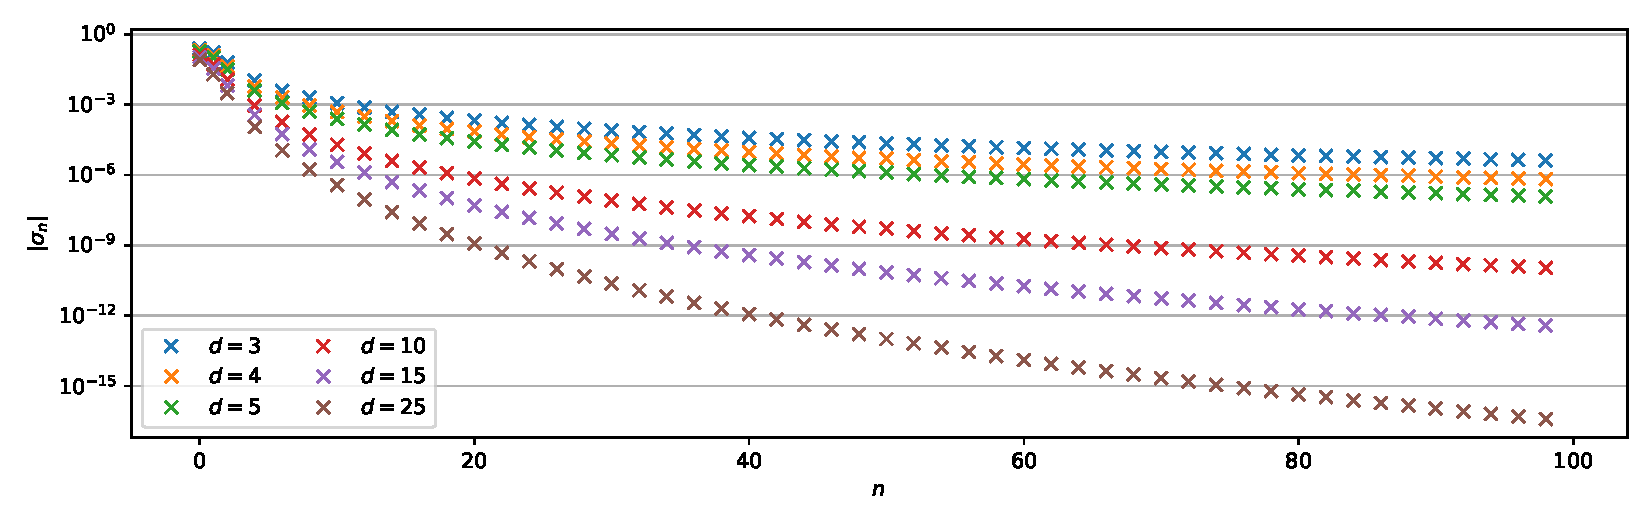
\includegraphics[width=\linewidth]{Appendix2/coefficients_relu.pdf}
    \caption{ReLU coefficients $\sigma_n$ as a function of degree $n$ for different dimensions $d$.}
    \label{fig:relu-coef}
\end{figure}

% \begin{figure}[t]
%     \centering
%     \includegraphics[width=\linewidth]{figures/spectra_kernels_and_activations.pdf}
%     \caption{Spectra of Arc Cosine and Mat\'ern-5/2 (blue), and ReLU and Softplus (orange) for different levels.}
%     \label{fig:spectra}
% \end{figure}

\end{appendices}

% *************************************** Index ********************************
\printthesisindex % If index is present

\end{document}
